\RequirePackage[l2tabu,orthodox]{nag}

% decide if one-sided/two-sided
%\documentclass[headsepline,footinclude=false,fontsize=11pt,paper=a4,listof=totoc,bibliography=totoc,BCOR=12mm,DIV=12]{scrbook} % two-sided
\documentclass[headsepline,footinclude=false,oneside,fontsize=11pt,paper=a4,listof=totoc,bibliography=totoc]{scrbook} % one-sided

\PassOptionsToPackage{table,svgnames,dvipsnames}{xcolor}

\usepackage[utf8]{inputenc}
\usepackage[T1]{fontenc}
\usepackage[sc]{mathpazo}
\usepackage[american]{babel}
\usepackage[autostyle]{csquotes}
\usepackage[%
  backend=biber,
  url=false,
  style=alphabetic,
  maxnames=4,
  minnames=3,
  maxbibnames=99,
  firstinits,
  uniquename=init]{biblatex} % adapt citation style
\usepackage{graphicx}
\usepackage[export]{adjustbox}
\usepackage{scrhack} % necessary for listings package
\usepackage{listings}
\usepackage{accsupp}
\usepackage{lstautogobble}
\usepackage{tikz}
\usepackage{pgfplots}
\usepackage{pgfplotstable}

\usetikzlibrary{shapes.misc}
\tikzset{cross/.style={cross out, draw=black, minimum size=2*(#1-\pgflinewidth), inner sep=0pt, outer sep=0pt},
%default radius will be 1pt. 
cross/.default={1pt}}

\usepackage{booktabs}
\usepackage[final]{microtype}
\usepackage[font=small]{caption} % smaller captions
\usepackage[hidelinks]{hyperref} % hidelinks removes colored boxes around references and links
\usepackage[super]{nth}
\usepackage{amsmath}
\usepackage{amssymb}
\usepackage{mathrsfs}
\usepackage{breqn}
\usepackage{caption}
\usepackage{subcaption}
%\usepackage{showframe} % use this for debugging the layout

% adjust default page margins
\usepackage[bottom=4.1cm, top=4.1cm]{geometry}

% package for thousand seperation
\usepackage[group-separator={,}]{siunitx}


\bibliography{bibliography}

\setkomafont{disposition}{\normalfont\bfseries} % use serif font for headings
\linespread{1.1} % adjust line spread for mathpazo font

% Settings for pgfplots
\pgfplotsset{compat=1.9} % adjust to your installed version
\pgfplotsset{
  % For available color names, see http://www.latextemplates.com/svgnames-colors
  cycle list={CornflowerBlue\\Dandelion\\ForestGreen\\BrickRed\\},
}

% Settings for lstlistings
\usepackage{inconsolata}
\usepackage{color}
\definecolor{pgrey}{rgb}{0.46,0.45,0.48}
\lstset{%
  basicstyle=\footnotesize\ttfamily,
  columns=fullflexible,
  autogobble,
  keywordstyle=\bfseries\color{MediumBlue},
  stringstyle=\color{DarkRed},
  commentstyle=\color{DarkGreen}\ttfamily,
  backgroundcolor=\color{gray!7},%
  numbers=left, numberstyle=\tiny,
  numberstyle=\tiny,
  tabsize=2,
  breaklines=true,
  showtabs=false,
  captionpos=b
  stepnumber=1,
  numbersep=9pt,
  frame=single,
  resetmargins=true
}
\lstdefinelanguage{PythonEx}{
  language     = Python,
  morekeywords = {with, as},
  moredelim=[is][\textcolor{pgrey}]{\%\%}{\%\%}
}



% Completely prevent breaking of footnotes over multiple pages
\interfootnotelinepenalty=10000 
\clubpenalty = 10000
\widowpenalty = 10000 
\displaywidowpenalty = 10000

% Math commands
\DeclareMathAlphabet\mathbfcal{OMS}{cmsy}{b}{n}
\newcommand\floor[1]{\lfloor#1\rfloor}
\newcommand\ceil[1]{\lceil#1\rceil}

\makeatletter
\newcommand{\Spvek}[2][r]{%
  \gdef\@VORNE{1}
  \left(\hskip-\arraycolsep%
    \begin{array}{#1}\vekSp@lten{#2}\end{array}%
  \hskip-\arraycolsep\right)}

\def\vekSp@lten#1{\xvekSp@lten#1;vekL@stLine;}
\def\vekL@stLine{vekL@stLine}
\def\xvekSp@lten#1;{\def\temp{#1}%
  \ifx\temp\vekL@stLine
  \else
    \ifnum\@VORNE=1\gdef\@VORNE{0}
    \else\@arraycr\fi%
    #1%
    \expandafter\xvekSp@lten
  \fi}
\makeatother

% custom spacing
\setlength{\parindent}{0em}
\setlength{\parskip}{0.5em}

% Glossary
\usepackage[acronym,automake, nonumberlist, toc]{glossaries}

% custom acronym table style:
\newglossarystyle{myacro}
{
	\renewenvironment{theglossary}{}{}
	\renewcommand*{\glossaryheader}{}
	\renewcommand*{\glsgroupheading}[1]{}
	\renewcommand*{\glsgroupskip}{}
	\renewcommand*{\glossaryentryfield}[5]
	{
		\begin{minipage}[t]{0.2\textwidth}
			\glstarget{##1}{##2}~\dotfill
		\end{minipage}
		\begin{minipage}[t]{0.7\textwidth}
			~##3
		\end{minipage}
		\vskip -0.16cm  % Abstand zwischen den Zeilen
	}
	\renewcommand*{\glossarysubentryfield}[6]{%
	\glossaryentryfield{##2}{##3}{##4}{##5}{##6}}%
}

% custom symbol table style:
\usepackage{multicol}
\newglossarystyle{mysymbol}
{
	\renewenvironment{theglossary}
	{\begin{multicols}{2}\noindent}{\end{multicols}}
	\renewcommand*{\glossaryheader}{}
	\renewcommand*{\glsgroupheading}[1]{}
	\renewcommand*{\glsgroupskip}{}
	\renewcommand*{\glossaryentryfield}[3]
	{\noindent
		\begin{minipage}[t]{0.94\columnwidth}
			\begin{minipage}[t]{0.2\columnwidth}
				\glstarget{##1}{##2}
			\end{minipage}
			\begin{minipage}[t]{0.78\columnwidth}
				##3
			\end{minipage}
		\end{minipage}
		\vskip 0.01em   % Abstand zwischen den Zeilen
	}
	\renewcommand*{\glossarysubentryfield}[3]{%
	\glossaryentryfield{##2}{##3}}%
}

% create symbol table
\newglossary[slg]{symbolslist}{syi}{syg}{List of Symbols}
% remove auto-dot at the end of every description
\renewcommand*{\glspostdescription}{}

% Empty pages for cleardoublepage:
% Start new chapter always on RHS page, so put in an additional
% blank page only when needed.
\usepackage{emptypage}
\newcommand{\skippage}{\newpage{\thispagestyle{empty}\mbox{}}}

% rotate figures
\usepackage{rotating}



% global pgf plot settings:
\pgfplotsset{
  every tick label/.append style={font=\tiny},
  label style = {font=\small},
  legend style = {font=\footnotesize}
}

% Import generated TUM logo (taken from http://www11.in.tum.de/lehre/thesis/latex)
% This is tumlogo.tex
%
% Neues TUM-Logo in TeX
%   by G. Teege, 19.10.89
% Benutzung:
%   Am Anfang des Dokuments (TeX oder LaTeX):
%     \input tumlogo
%   Dann beliebig oft:
%     \TUM{<breite>}
%   bzw.
%     \oTUM{<breite>}
%   \TUM setzt das Logo mit der Breite <breite> und der entsprechenden Hoehe.
%   <breite> muss eine <dimen> sein. \oTUM erzeugt eine "outline"-Version
%   des Logos, d.h. weiss mit schwarzem Rand. Bei \TUM ist es ganz schwarz.
%   \oTUM entspricht damit der offiziellen Version des Logos.
%   Das Logo kann wie ein einzelnes Zeichen verwendet werden.
%   Beispiel:
%     Dies ist das TUM-Logo: \oTUM{1cm}.
%
\def\TUM#1{%
\dimen1=#1\dimen1=.1143\dimen1%
\dimen2=#1\dimen2=.419\dimen2%
\dimen3=#1\dimen3=.0857\dimen3%
\dimen4=\dimen1\advance\dimen4 by\dimen2%
\setbox0=\vbox{\hrule width\dimen3 height\dimen1 depth0pt\vskip\dimen2}%
\setbox1=\vbox{\hrule width\dimen1 height\dimen4 depth0pt}%
\setbox2=\vbox{\hrule width\dimen3 height\dimen1 depth0pt}%
\setbox3=\hbox{\copy0\copy1\copy0\copy1\box2\copy1\copy0\copy1\box0\box1}%
\leavevmode\vbox{\box3}}
%
\def\oTUM#1{%
\dimen1=#1\dimen1=.1143\dimen1%
\dimen2=#1\dimen2=.419\dimen2%
\dimen3=#1\dimen3=.0857\dimen3%
\dimen0=#1\dimen0=.018\dimen0%
\dimen4=\dimen1\advance\dimen4 by-\dimen0%
\setbox1=\vbox{\hrule width\dimen0 height\dimen4 depth0pt}%
\advance\dimen4 by\dimen2%
\setbox8=\vbox{\hrule width\dimen0 height\dimen4 depth0pt}%
\advance\dimen4 by-\dimen2\advance\dimen4 by-\dimen0%
\setbox4=\vbox{\hrule width\dimen4 height\dimen0 depth0pt}%
\advance\dimen4 by\dimen1\advance\dimen4 by\dimen3%
\setbox6=\vbox{\hrule width\dimen4 height\dimen0 depth0pt}%
\advance\dimen4 by\dimen3\advance\dimen4 by\dimen0%
\setbox9=\vbox{\hrule width\dimen4 height\dimen0 depth0pt}%
\advance\dimen4 by\dimen1%
\setbox7=\vbox{\hrule width\dimen4 height\dimen0 depth0pt}%
\dimen4=\dimen3%
\setbox5=\vbox{\hrule width\dimen4 height\dimen0 depth0pt}%
\advance\dimen4 by-\dimen0%
\setbox2=\vbox{\hrule width\dimen4 height\dimen0 depth0pt}%
\dimen4=\dimen2\advance\dimen4 by\dimen0%
\setbox3=\vbox{\hrule width\dimen0 height\dimen4 depth0pt}%
\setbox0=\vbox{\hbox{\box9\lower\dimen2\copy3\lower\dimen2\copy5%
\lower\dimen2\copy3\box7}\kern-\dimen2\nointerlineskip%
\hbox{\raise\dimen2\box1\raise\dimen2\box2\copy3\copy4\copy3%
\raise\dimen2\copy5\copy3\box6\copy3\raise\dimen2\copy5\copy3\copy4\copy3%
\raise\dimen2\box5\box3\box4\box8}}%
\leavevmode\box0}
% End of tumlogo.tex



\newcommand*{\getUniversity}{Technische Universität München}
\newcommand*{\getFaculty}{Department of Informatics}
\newcommand*{\getTitle}{Deep Learning Approaches\\to Predict Future Frames in Videos}
\newcommand*{\getTitleGer}{Herangehensweisen in Deep Learning\\zur Vorhersage von Zukünftigen Bildern\\in Videos}
\newcommand*{\getAuthor}{Benjamin Sautermeister}
\newcommand*{\getDoctype}{Master's Thesis in Computer Science}
\newcommand*{\getSupervisor}{Prof. Dr. Daniel Cremers}
\newcommand*{\getAdvisor}{Philip Häusser}
\newcommand*{\getSubmissionDate}{\nth{17} October, 2016} % American format: https://www.englishclub.com/vocabulary/time-date.htm
\newcommand*{\getSubmissionLocation}{Munich}

% commands
\newcommand{\abk}[1]{\glslink*{#1}{#1}}	% prints acronym
\newcommand{\addabk}[2]{\newacronym{#1}{#1}{#2}} % adds acronym entry (preamle only)


% ACRONYMS
\addabk{ANN}{\textbf{A}rtificial \textbf{N}eural \textbf{N}etwork}
\addabk{NN}{\textbf{N}eural \textbf{N}etwork}
\addabk{CNN}{\textbf{C}onvolutional \textbf{N}eural \textbf{N}etwork}
\addabk{RNN}{\textbf{R}ecurrent \textbf{N}eural \textbf{N}etwork}
\addabk{FCN}{\textbf{F}ully-\textbf{C}onvolutional \textbf{N}etwork}
\addabk{AI}{\textbf{A}rtificial \textbf{I}ntelligence}
\addabk{ML}{\textbf{M}achine \textbf{L}earning}
\addabk{LSTM}{\textbf{L}ong \textbf{S}hort-\textbf{T}erm \textbf{M}emory}
\addabk{FC-LSTM}{\textbf{F}ully-\textbf{C}onnected \textbf{LSTM}}
\addabk{ConvLSTM}{\textbf{Conv}olutional \textbf{LSTM}}
\addabk{MLP}{\textbf{M}ulti\textbf{l}ayer \textbf{P}erceptron}
\addabk{FC}{\textbf{F}ully-\textbf{C}onnected}
\addabk{RGB}{\textbf{R}ed \textbf{G}reen \textbf{B}lue}
\addabk{MAE}{\textbf{M}ean \textbf{A}bsolute \textbf{E}rror}
\addabk{MSE}{\textbf{M}ean \textbf{S}quared \textbf{E}rror}
\addabk{BCE}{\textbf{B}inary \textbf{C}ross-\textbf{E}ntropy}
\addabk{ReLU}{\textbf{R}ectified \textbf{L}inear \textbf{U}nit}
\addabk{SDG}{\textbf{S}tochastic \textbf{G}radient \textbf{D}escent}
\addabk{OCR}{\textbf{O}ptical \textbf{C}haracter \textbf{R}ecognition}
\addabk{DCGAN}{\textbf{D}eep \textbf{C}onvolutional \textbf{G}enerative \textbf{A}dversarial \textbf{N}etwork}
\addabk{GAN}{\textbf{G}enerative \textbf{A}dversarial \textbf{N}etwork}
\addabk{BRNN}{\textbf{B}idirectional \textbf{R}ecurrent \textbf{N}eural \textbf{N}etwork}
\addabk{BPTT}{\textbf{B}ack\textbf{p}ropagation \textbf{T}hrough \textbf{T}ime}
\addabk{GRU}{\textbf{G}ated \textbf{R}ecurrent \textbf{U}nit}
\addabk{PSNR}{\textbf{P}eak \textbf{S}ignal-to-\textbf{N}oise \textbf{R}atio}
\addabk{FR}{\textbf{F}ull \textbf{R}eference}
\addabk{SSIM}{\textbf{S}tructural \textbf{Sim}ilarity}
\addabk{MS-SSIM}{\textbf{M}ulti-\textbf{S}cale \textbf{S}tructural \textbf{Sim}ilarity}
\addabk{JPEG}{\textbf{J}oint\textbf{ P}hotographic \textbf{E}xperts \textbf{G}roup}
\addabk{GDL}{\textbf{G}radient \textbf{D}ifference \textbf{L}oss}
\addabk{MNIST}{\textbf{M}ixed \textbf{N}ational \textbf{I}nstitute of \textbf{S}tandards and \textbf{T}echnology}
\addabk{UCF}{\textbf{U}niversity of \textbf{C}entral \textbf{F}lorida}
\addabk{PCA}{\textbf{P}rinciple \textbf{C}omponent \textbf{A}nalysis}
\addabk{Adam}{\textbf{Ad}aptive \textbf{M}oments \textbf{E}stimation}
\addabk{API}{\textbf{A}pplication \textbf{P}rogramming \textbf{I}nterface}
\addabk{TUM}{\textbf{T}echnische \textbf{U}niversität \textbf{M}ünchen}
\addabk{MIT}{\textbf{M}assachusetts \textbf{I}nstitute of \textbf{T}echnology}
\addabk{JSON}{\textbf{J}ava\textbf{S}cript \textbf{O}bject \textbf{N}otation}
\addabk{GPU}{\textbf{G}raphics \textbf{P}rocessing \textbf{U}nit}
\addabk{CPU}{\textbf{C}entral \textbf{P}rocessing \textbf{U}nit}
\addabk{GIF}{\textbf{G}raphics \textbf{I}nterchange \textbf{F}ormat}


% GLOSSARY
%\newglossaryentry{test} {
%  name={TestTest},
%  description={The test description gloss entry.},
%}


% MATH SYMBOLS
\newglossaryentry{hadamard}{name=\ensuremath{\odot},
        description={Hadamard product},
		type=symbolslist}
\newglossaryentry{input}{name=\ensuremath{x_{i}},
        description={Input element},
		type=symbolslist}
\newglossaryentry{output}{name=\ensuremath{y_{i}},
        description={Output element},
		type=symbolslist}
\newglossaryentry{weight}{name=\ensuremath{W_{i}},
        description={Weight element},
		type=symbolslist}
\newglossaryentry{bias}{name=\ensuremath{b},
        description={Bias (or negative threshold)},
		type=symbolslist}
\newglossaryentry{activ}{name=\ensuremath{\phi(x)},
        description={Activation function},
		type=symbolslist}
\newglossaryentry{lr}{name=\ensuremath{\eta},
        description={Learning rate},
		type=symbolslist}
\newglossaryentry{loss}{name=\ensuremath{\mathcal{L}(x)},
        description={Loss function},
		type=symbolslist}
\newglossaryentry{reg}{name=\ensuremath{\lambda},
        description={Regularization coefficient},
		type=symbolslist}
\newglossaryentry{hidden}{name=\ensuremath{h^{(\tau)}},
        description={Hidden state at time step $\tau$},
		type=symbolslist}
\newglossaryentry{cellstate}{name=\ensuremath{C^{(\tau)}},
        description={Cell state at time step $\tau$},
		type=symbolslist}
\newglossaryentry{l_one}{name=\ensuremath{\ell_1},
        description={Least absolute deviations},
		type=symbolslist}
\newglossaryentry{l_two}{name=\ensuremath{\ell_2},
        description={Least square errors},
		type=symbolslist}
\newglossaryentry{conv}{name=\ensuremath{\ast},
        description={Convolution operation},
		type=symbolslist}
\newglossaryentry{sigmoid}{name=\ensuremath{\sigma(x)},
        description={Sigmoid activation function},
		type=symbolslist}
\newglossaryentry{argmin}{name=\ensuremath{\textrm{arg}\min\limits_{x}},
        description={Value of $x$ for which the minimum is attained},
		type=symbolslist}
\newglossaryentry{uniform}{name=\ensuremath{\textrm{U}},
        description={Uniform distribution},
		type=symbolslist}
\newglossaryentry{matr_elem}{name=\ensuremath{\textbf{X}_{c,r}},
        description={Element at column $c$ and row $r$ of matrix $X$},
		type=symbolslist}
\newglossaryentry{grad}{name=\ensuremath{\nabla},
        description={Gradient},
		type=symbolslist}
\newglossaryentry{dim}{name=\ensuremath{d_x},
        description={Dimensionality of $x$},
		type=symbolslist}
\newglossaryentry{reg_term}{name=\ensuremath{\Omega(x)},
        description={Regularizer term},
		type=symbolslist}
\newglossaryentry{var}{name=\ensuremath{Var(x)},
        description={Variance of $x$},
		type=symbolslist}
\newglossaryentry{expvalue}{name=\ensuremath{\mathbb{E}(x)},
        description={Expectation value of $x$},
		type=symbolslist}
\newglossaryentry{max_poss}{name=\ensuremath{\textbf{x}_{max}},
        description={Maximum possible value of $x$},
		type=symbolslist}
\newglossaryentry{mu}{name=\ensuremath{\mu_x},
        description={Mean value of $x$},
		type=symbolslist}
\newglossaryentry{sigma}{name=\ensuremath{\sigma_x},
        description={Standard deviation of $x$},
		type=symbolslist}
\newglossaryentry{stride}{name=\ensuremath{s},
        description={Stride value},
		type=symbolslist}
\newglossaryentry{padding}{name=\ensuremath{p},
        description={Padding value / probability},
		type=symbolslist}
\newglossaryentry{kernel}{name=\ensuremath{k},
        description={Kernel size value},
		type=symbolslist}
\newglossaryentry{time}{name=\ensuremath{\tau},
        description={Time step},
		type=symbolslist}
\newglossaryentry{corrupt}{name=\ensuremath{\tilde{x}},
        description={Corrupted value of $x$},
		type=symbolslist}
		





\makeglossaries

\begin{document}

% Set page numbering to avoid "destination with the same identifier has been already used" warning for cover page.
% (see https://en.wikibooks.org/wiki/LaTeX/Hyperlinks#Problems_with_Links_and_Pages).
\pagenumbering{alph}
\begin{titlepage}
  % HACK for two-sided documents: ignore binding correction for cover page.
  % Adapted from Markus Kohm's KOMA-Script titlepage=firstiscover handling.
  % See http://mirrors.ctan.org/macros/latex/contrib/koma-script/scrkernel-title.dtx,
  % \maketitle macro.
  \oddsidemargin=\evensidemargin\relax
  \textwidth=\dimexpr\paperwidth-2\evensidemargin-2in\relax
  \hsize=\textwidth\relax

  \centering

  \IfFileExists{logos/tum.pdf}{%
    \includegraphics[height=20mm]{logos/tum.pdf}
  }{%
    \vspace*{20mm}
  }

  \vspace{5mm}
  {\huge\MakeUppercase{\getFaculty{}}}\\

  \vspace{5mm}
  {\large\MakeUppercase{\getUniversity{}}}\\

  \vspace{20mm}
  {\Large \getDoctype{}}

  \vspace{15mm}
  {\huge\bfseries \getTitle{}}

  \vspace{15mm}
  {\LARGE \getAuthor{}}

  \IfFileExists{logos/faculty.pdf}{%
    \vspace{20mm}
    \includegraphics[height=20mm]{logos/faculty.pdf}
  }{}
\end{titlepage}


\frontmatter{}

\begin{titlepage}
  \centering

  \IfFileExists{logos/tum.pdf}{%
    \includegraphics[height=20mm]{logos/tum.pdf}
  }{%
    \vspace*{20mm}
  }

  \vspace{5mm}
  {\huge\MakeUppercase{\getFaculty{}}}\\

  \vspace{5mm}
  {\large\MakeUppercase{\getUniversity{}}}\\

  \vspace{20mm}
  {\Large \getDoctype{}}

  \vspace{15mm}
  {\huge\bfseries \getTitle{}}

  \vspace{10mm}
  {\huge\bfseries \getTitleGer{}}

  \vspace{15mm}
  \begin{tabular}{l l}
    Author: & \getAuthor{} \\
    Supervisor: & \getSupervisor{} \\
    Advisor: & \getAdvisor{} \\
    Submission Date: & \getSubmissionDate{} \\
  \end{tabular}

  \IfFileExists{logos/faculty.pdf}{%
    \vfill{}
    \includegraphics[height=20mm]{logos/faculty.pdf}
  }{}
\end{titlepage}

\thispagestyle{empty}
\vspace*{0.8\textheight}
\noindent
I confirm that this \MakeLowercase{\getDoctype{}} is my own work and I have documented all sources and material used.

\vspace{15mm}
\noindent
\getSubmissionLocation{}, \getSubmissionDate{} \hspace{50mm} \getAuthor{}

\cleardoublepage{}

\addcontentsline{toc}{chapter}{Acknowledgments}
\thispagestyle{empty}

\vspace*{20mm}

\begin{center}
{\usekomafont{section} Acknowledgments}
\end{center}

\vspace{10mm}

I would like to express my sincere thanks to those who offered feedback on the content or made this thesis even possible. Beginning with \textit{Prof. Dr. Daniel Cremers} for his valuable suggestions at the very beginning of my work. Next, my advisor \textit{Philip Häusser} for offering this interesting topic, his continuous support as well as our fruitful discussion at Google Zurich. Furthermore, I would like to acknowledge \textit{PD Dr. habil. Rudolph Triebel} for his tough but outstanding lecture \textit{Machine Learning in Computer Vision} at TUM, which initiated my interest to do a thesis in this field.


Last but not least, I would also like to thank my family for their faith and positive mentality, who waited patiently for me to finish this work. And not forgetting \textit{Shiv Baishya}, \textit{Tom Kingdom}, \textit{Stefan Kraus}, \textit{Patrick Mutter}, \textit{Manuel Sautermeister} and \textit{Lukas Wöhrl} for investing their time in proofreading this thesis.

\cleardoublepage{}

\chapter{\abstractname}

Deep networks are becoming central in several areas of computer vision and image processing task. But while there has been a lot of research regading classification of images or videos, future frame prediction is still a rarely studied approach. However, many applications could make good use of the knowledge regarding the next frame of a video in pixel-space, such as video compression or autonomous agents in robotics that have to act in natural environments. In fact learning how to forecast the future of an image sequence requires the system to understand and efficiently encode the conent and dynamics for a certein period of time. Furthermore, it is viewed as a promising avenue where even supervised tasks could benefit from, because large datasets of labeled video data are limited and very hard to obtain. Therefore, an overview of existing approaches that cover future frame prediction is given and a new network model is presented which utilzes recent advances from deep learning research. The proposed architecture is based on the recurrent decoder-endocder framework with convolutional cells which allow to preserve spatio-temporal correlations of the data. Driven by perceptual motivated objective functions and new recurrent learning strategy, it is able to outperform many existing approaches in several types of videos, even though it is trained for fewer iterations and contains fewer model parameters.
\microtypesetup{protrusion=false}
\tableofcontents{}
\microtypesetup{protrusion=true}

\mainmatter{}

% !TeX root = ../main.tex


\chapter{Introduction} \label{chapter:introduction}

Since the classical era, people have dreamed of inventing machines that can act and think like humans. This opened the field of \textit{artificial intelligence} (AI), which is still an active research topic and is used in many practical applications. The main focus of AI in early days was to solve problems that are hard to solve for humans, such as finding the shortest path to an arbitrary destination using the well-known \textit{Dijkstra algorithm}\footnote{Also known as uniform-cost search}. Ironically, it turned out that tasks which can be solved by humans using pure intuition are actually extremely hard for computers to solve. As an example, it is hard or even impossible to write a program from scratch that is able to detect objects in pictures, recognize words in spoken text or to describe the events in a video scene. The reason is that classical computer programs in contrast have to be algorithmically expressed as a sequence of commands or a list of mathematical rules \parencite{deep_learning}. But it is quite tough to apply this on multi-dimensional data such as pictures or videos that consists of an incoherent set of pixels including different color channels with a lot of noise and countless possibilities. 

Humans handle this kind of data differently. They learn to recognize objects by experience and implicitly build hierarchies of relationships in their mind. This basic principle opened a new subfield, known as \textit{machine learning} (ML). It covers a methodology where knowledge is acquired by extracting patterns from raw data and consequently allows to make reasonable decisions \parencite{deep_learning}. But while this is able to cover many previously unsolvable problems, it requires that one can tell which features we would like to investigate, for instance to build a decision tree out of it. Coming back to our previous example, this is still hard to be applied on images or video data where we might know which features we are looking for, but still cannot formally describe how these are represented. A field that deals with this issue is called \textit{representation learning}, which tries to automatically build the representation by itself.

Having just a high-level representation might still not be enough. To break down the problem, \textit{artificial neural networks} (ANN) have been introduced. They are biologically inspired by the structure of the human brain \parencite{ann} and can be trained to learn hierarchies of representations. For object recognition on images, we can think of edges that are detected on a very low level, which will be further composed to curves or shapes. Furthermore, these simple structures might be compound in a specific way, so that the neural network can identify distinct complex objects in it. The rise of computational power allows to create networks that are even deeper and therefore learn more and more complex representations hierarchies. This principle caused its contemporary name, known as \textit{deep learning}.

\section{Motivation}

In recent years, the field of deep learning achieved considerable success and according to its underlying philosophy: ``\textit{if we have a reasonable end-to-end model and sufficient data for training it, we are close to solving the problem.}'' \parencite{conv_lstm_nowcasting}. But while there has been a lot of studies and practical applications of object recognition on static images or speech recognition, the application of these concepts on video data are just about to make their first steps in research. 

Early deep learning approaches dealing with video data or simple image sequences address problems like human action recognition \parencite{conv3d_action_class}, \parencite{two_stream_action}, \parencite{longterm_rec_recog} or video classification \parencite{large_video_class}. Another example is optical flow prediction \parencite{flownet} in order to detect the visual flow from one frame to the next. Most of these approaches require lots of labeled data to be able to train a network. The effortful labeling process and thus the resulting low availability of such data might be the main reason why this topic has not been covered that well so far. On the contrary, online services like \textit{YouTube} provide a seemingly endless, but unlabeled source of videos to learn from.


\section{Problem Statement}

Throughout this work, we would like to investigate whether deep learning techniques can be successfully applied on videos to learn a meaningful representation in a completely unsupervised fashion. In detail, we would like to examine if such a representation is suited to continue a video even after it has finished. Hence, to learn a notion of the spatial and temporal evolution within a sequence of images as well as to get an idea of motion and dynamics of a scene. Such a high-level understanding would be helpful for autonomous intelligent agents that have to act and therefore understand our environment including its physical and temporal constrains \parencite{unsup_learn_lstm}. Other application areas might be for instance video compression \parencite{frame_interpol}, visual systems for autonomous cars or as a replacement for optical flow in causal video segmentation \parencite{causal_video_seg}. Aside from that, other supervised learning tasks like human action recognition could benefit from such a pre-trained network in order to improve the overall performance or to reduce the training time. Needless to say, other forms of \textit{transfer learning} are easily conceivable as well.

\begin{figure}[htpb]
	\centering
	
\includegraphics[width=1.0\linewidth]{figures/ucf-intro/serie1.png} 
	\caption[Example Image Sequence]{Example of an image sequence with an unknown future frame. The sequence is starting from the left and is taken from UCF-101.} \label{fig:intro-seq}
\end{figure}

Like in the first example of object recognition on static pictures, this task might sound trivial for humans once more, since we already have built an intuition regarding motion and our environment. When we have a look at the image sequence in Figure \ref{fig:intro-seq}, we have a strong idea about how this sequence might continue. At least for a couple of time steps. The boy in the foreground probably will lift his left foot towards the ball, while the ball continues to fall down due to gravitation. In contrast, the background will stay almost unchanged.

Developing a deep learning approach to tackle this is indeed a non-trivial task, since it has to model both spatial and temporal features in combination, as well as the search space grows exponential in case of multi-step forecasting. Additionally, related issues like evolving an effective training process or quantifying the perceptual image similarity between predicted and the ground truth frames have to be addressed as well. Moreover, existing state-of-the-art implementations that deal with frame prediction have to be reviewed and analyzed in detail in order to learn from their strength and weaknesses.


\section{Contributions}

This thesis consists of several contributions. Firstly, it provides a dense \textit{overview} of existing deep learning approaches that deal with the problem of future frame prediction in videos. Secondly, it presents a neural network architecture that combines modern practices like \textit{batch normalization} with a novel \textit{convolutional LSTM} implementation and \textit{scheduled sampling} to improve training of recurrent models. Thereby, it is able to \textit{cut in half the prediction error} of other state-of-the-art models in the MovingMNIST dataset. Last but not least, we make all of our TensorFlow implementations available to the research community, including our scheduled sampling and batch normalization enabled convolutional recurrent cell, as well as several metrics and loss functions to measure perceptual image similarity at training time. Furthermore, we contribute a \textit{lightweight, high-level and open source framework for TensorFlow} that is able to radically reduce boilerplate code of deep learning applications. This is facilitated by providing an abstraction for many recurring or complex tasks that have to be faced while building and training neural network models.


\section{Organization}

The subsequent chapters of this thesis are structured as followed:

\textbf{Chapter \ref{chapter:fundamentals}} covers the theoretical concepts that are required to understand our final implementation and its consecutive evaluation. We will have a deeper look into neural networks and explain how they are trained. Further, we explore more advanced neural network architectures, namely \textit{convolutional neural networks} (CNN) for spatial learning and \textit{recurrent neural network} (RNN) models for sequential learning. Afterwards, this chapter concludes with the investigation of some modern techniques that are used to improve the overall learning process, as well as metrics for perceptual motivated image similarity assessment.

In \textbf{Chapter \ref{chapter:relatedwork}}, a closer look is taken at existing approaches that are suitable for spatio-temporal learning and frame prediction. It briefly discusses their strength and weaknesses, as well as how they have influenced the design decisions regarding the architecture of the final neural network model. Additionally, these models build the baselines in the evaluation.

Afterwards, the implemented neural network model is presented in \textbf{Chapter \ref{chapter:implementation}}, including its architecture and implementation details. Moreover, a quite recently invented and barely studied variant of recurrent network cell for spatio-temporal learning, namely \textit{convolutional LSTM}, is introduced which builds the central element of the realized model. It also suggests a special learning strategy for RNNs, which speeds up the training process and enables improvement of the overall performance.

\textbf{Chapter \ref{chapter:datasets}} gives a brief overview of the video datasets used within this thesis. All in all, three different sets with increasing complexity have been chosen, namely \textit{Moving MNIST}, \textit{MsPacman} and \textit{UCF-101}.

Next, \textbf{Chapter \ref{chapter:evaluation}} illustrates many experimental results on the previously named datasets. It investigates how changes in the model or hyperparameters do affect the model's performance, as well as compares the results with other existing approaches in detail.

Within \textbf{Chapter \ref{chapter:contribution}}, a lightweight, high-level framework for \textit{TensorFlow} is presented as a side contribution that has grown out of this project.

In the end, this thesis is concluded in \textbf{Chapter \ref{chapter:conclusion}} by summarizing the overall results, as well as highlight the identified possible improvements for future work.




% !TeX root = ../main.tex

% FURTHER IDEAS:
% - data augmentation
% - data preprocessing

\chapter{Fundamentals} \label{chapter:fundamentals}

To get a general understanding of how training a neural network works, this chapter goes through its theoretical concepts first. It starts with the structure of simple feed-forward networks, continue with advanced model architectures that take advantage of the data's spatial or temporal properties. And finally it ends up with recent techniques that are used throughout the final implementation.


\section{Neural Networks}

The main concept of \textit{neural networks} (NN) dates back to the early 1950s, when Warren McCulloch and Walter Pitts tried to build a mathematical model of information processing in our brain. Inspired by this work, Frank Rosenblatt developed the so called \textit{perceptron} about two decades later \parencite[p. 226]{pattern_and_ml}. 

\subsection{Basics}

The perceptron itself has quite a simple structure. It is usually visualized as a node that has any number of binary inputs $ x_{i} $, as well as a single output $ y $ with $ x_{i}, y \in \{0, 1\} $. In addition, each input is weighted by $ w_{i} \in \mathbb{R} $ to express the importance of each particular input. The output is determined by the simple rule that the weighted sum of all inputs has to reach a specified threshold to make the perceptron fire its output \parencite{neural_nets_deep_learning}. This threshold is usually called bias $ b \in \mathbb{R} $, defined as the negative threshold. All of this can be expressed as follows:

\begin{equation} \label{eq:mlp}
  y = \begin{cases}
    1, & \text{if $ \sum\limits_{i=1}^n \, w_{i} \, x_{i} + b > 0$},\\
    0, & \text{otherwise}.
  \end{cases}
\end{equation}

Even that its formulation is that simple, it can represent complex decision-making when multiple elements are stacked together, known as a multilayer perceptron (MLP). Such a network forms a \textit{directed acyclic graph} (DAG) and is illustrated in Figure \ref{fig:mlp}.

\begin{figure}[htpb]
	\centering
	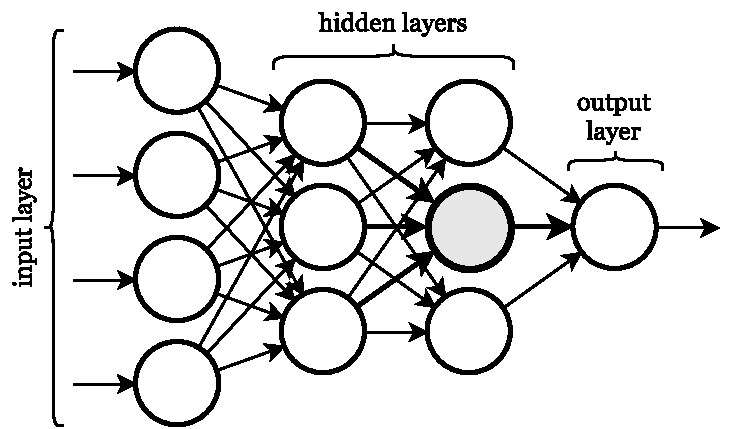
\includegraphics[width=.75\linewidth]{figures/mlp.pdf}
	\caption[Multilayer Perceptron]{Example of a MLP with two hidden layers. A single perceptron is highlighted in bold. (Based on \parencite{neural_nets_deep_learning})} \label{fig:mlp}
\end{figure}

The first and last layer of such a network are referred to as \textit{input layer} and \textit{output layer}. Furthermore, the number of nodes is determined by the given problem to solve. In case we want to train a network that identifies human faces in RGB-colored pictures with height and width of 100 pixels, it would require our input layer to have $ n_{in}=$ \num{30000} perceptrons, as well as a single output node. In contrary, all intermediate layers are known as \textit{hidden layers} and can have any number of elements and depth. When every node from one layer is connected to all nodes of its subsequent layer, it is called \textit{fully connected} (FC).

Afterwards, the input layer can be fed with a data example and apply equation \ref{eq:mlp} in each node to retrieve our binary result. This prediction step is called \textit{inference}. But in order to retrieve meaningful results, the network has to be trained first to have appropriate values for the weights and biases.

\subsection{Network Training}

The final goal of training such a network is to end up with a model that generalizes on any kind of data from the same type \parencite[p. 2]{pattern_and_ml}. Data that is used during this process is called \textit{training set}, the other portion of data that evaluates its generalization capabilities \textit{test set}. Additionally, a third split is preferably used during the training process of the networks to select the best performing approach. It is known as the \textit{validation set}. Since the ground truth outcome of each data example during the training phase is known, we can quantify the outcomes using a loss function\footnote{Often called cost function, objective function or error function as well.}, such as \textit{mean absolute error} (MAE)\footnote{Also known as $ \ell_1 $ when it does not average over all examples, but often used as a synonym. In this work, the averaged variants for all presented functions are always used. Additionally, we also average across the image pixels when any loss function is applied on images to achieve pixel-wise results that are independent regarding the image dimensions later on in context of frame prediction.}:

\begin{equation} \label{eq:mae}
  \mathcal{L}_{\textrm{mae}}(\textbf{w}, \textbf{b})=\frac{1}{n} \sum\limits_{\textbf{x}} | y(\textbf{x}) - t(\textbf{x}) | ,
\end{equation}

\textit{mean squared error} (MSE)\footnote{Also referred to as $ \ell_2 $ when no averaging across all examples is performed.}:

\begin{equation} \label{eq:mse}
  \mathcal{L}_{\textrm{mse}}(\textbf{w}, \textbf{b})=\frac{1}{n} \sum\limits_{\textbf{x}} ( y(\textbf{x}) - t(\textbf{x}) )^2 ,
\end{equation}

or \textit{binary cross-entropy} (BCE) \parencite{conv_lstm_nowcasting}:

\begin{equation} \label{eq:bce}
  \mathcal{L}_{\textrm{bce}}(\textbf{w}, \textbf{b})= -\frac{1}{n} \sum\limits_{\textbf{x}} t(\textbf{x}) \cdot \log{\big(y(\textbf{x})\big)} + \big(1-t(\textbf{x})\big) \cdot \log{\big(1-y(\textbf{x})\big)} ,
\end{equation}

where $ n $ is the number of examples and $ t(\textbf{x}) $ denotes a mapping from an input example $ \textbf{x} $ to its ground truth target. Many other functions exist and some more will be introduced in Section \ref{sec:perc-loss}, but the above listed formulas are the main objectives that are used in many other works. During training of the network, the set of weights $ \textbf{w} $ and biases $ \textbf{b} $ have to be found that minimizes the error:

\begin{equation} \label{eq:min-loss}
  \textrm{arg}\min_{\textbf{w}, \textbf{b}} \mathcal{L}(\textbf{w}, \textbf{b}) .
\end{equation}

Parameters beside $ \textbf{w} $ and $ \textbf{b} $ that are not learned during this process are called \textit{hyperparameters}. Examples of such non-trainable parameters are the number of layers or the size of each single hidden layer. More hyperparameters will arise throughout this chapter.


\subsubsection{Neurons and Activations}

At this point, the fundamental problem of perceptrons is faced. In order find the best set of parameters, small changes in the model's weights $ \textbf{w} $ and biases $ \textbf{b} $ have to be performed to justify the output into the right direction of the desired outcome. But since the perceptron's output is discrete, a small change can cause a sudden flip in the overall output of the model. To overcome this issue, these perceptrons are replaced with \textit{neurons}. The exemplary structure of a neuron is illustrated in Figure \ref{fig:neuron}. They are given by:

\begin{equation}
\begin{aligned}
z &= \sum\limits_{i=1}^n \, w_{i} \, x_{i} + b \\
y &= \phi(z) ,
\end{aligned}
\end{equation}

which allow $ x_{i}, y \in \mathbb{R} $ by wrapping its term with a non-linear \textit{activation function} $ \phi(z) $. Frequently used examples are the sigmoid function $ \sigma(z) $, hyperbolic tangent $ tanh(z) $ and the rectified linear unit (ReLU) $ max(0, z) $, illustrated in Figure \ref{fig:activations}.

\begin{figure}[htpb]
	\centering
	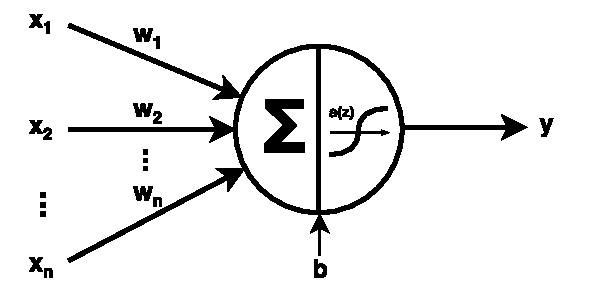
\includegraphics[width=.45\linewidth]{figures/neuron.pdf}
	\caption[Schematic Neuron]{Schematic structure of a neuron with its $ n $ inputs $x_{i}$, weights $w_{i}$, bias $ b $ and activation function $\phi(z)$.} \label{fig:neuron}
\end{figure}

Note that the sigmoid function's shape is a smoothed out variant of the \textit{step function} \parencite{neural_nets_deep_learning}, which can be used to make a neuron act like a classical perceptron. Additionally, the rectifier differs to both other activation functions in that it is one-sided and partly linear. Even that its shape looks much simpler, it became the most favorable activation function for intermediate layers in deep neural networks. The reasons are that it allows faster computation, sparse activation\footnote{{A sparse activation means that only half of the neurons have an initial non-zero output, when a uniform initialization is used.}}, reduces the likelihood of vanishing gradient (see Section \ref{sec:rnn-drawbacks}) and is more biologically plausible \parencite{relu}.

\begin{figure}[htpb]
  \centering
  \begin{tikzpicture}
    \begin{axis}[
        ymin=-1,
        ymax=2,
        xmin=-3,
        xmax=3,
        legend style={legend pos=south east},
        grid,
        thick,
        ylabel=a(z),
        xlabel=z
      ]
      \addplot [mark=none,draw=blue,smooth,ultra  thick] {1/(1+exp(-1*(\x))};
      \addlegendentry{sigmoid};
      \addplot [mark=none,draw=red,smooth,ultra thick] {tanh(\x)};
      \addlegendentry{tanh};
      \addplot[mark=none,draw=black!30!green,ultra thick,smooth,domain=0:3] {x};
	  \addplot[mark=none,draw=black!30!green,ultra thick,smooth,domain=-3:0] {0};
      \addlegendentry{ReLU};
    \end{axis}
  \end{tikzpicture}
  \caption[Activation functions]{Visualization of the most commonly used activation functions in neural networks.}\label{fig:activations}
\end{figure}

\subsubsection{Initialization}

Before starting the training process, an initial value is assigned to each variable $ \textbf{w} $ and $ \textbf{b} $. This is done by pure randomness, using for example a uniform or Gaussian distribution. But if we start with weights that are too small, the signal could decrease so much that it is too small to be useful. On the other side, when we initialize our parameters with high values, the signal can end up to explode while propagating through the network \parencite{understand_xavier}. In consequence, a good initialization can have a radical effect on how fast the network will learn useful patterns.

For this purpose, some best practices have been developed. One famous example used in our final model is \textit{Xavier initialization}\footnote{Also known as Glorot initialization.} (see eq. \ref{eq:xavier}). Its formulation is based on the number of input and output neurons and uses sampling from a uniform distribution with zero mean and all biases set to zero \parencite{xavier-init}:

\begin{equation} \label{eq:xavier}
  \textbf{w} \sim \textrm{U} \bigg[-\sqrt{\frac{6}{n_{in} + n_{out}}}, \sqrt{\frac{6}{n_{in} + n_{out}}}\bigg] ,
\end{equation}

where $ \textbf{w} $ is the weight matrix at any network layer, $ n_{in} $ the number of incoming connections and $ n_{out} $ the number of outgoing connections to the next layer. This initialization is designed to keep the gradients in all layers within approximately the same scale.

As an alternative to random initialization and performing a training of the entire network from scratch, it is also possible to reuse parts or even all trained parameters from a different model. A famous example that is often used to pre-initialize a network for image processing tasks is \textit{AlexNet} \parencite{imagenet}. It is pre-trained for several weeks across multiple graphic cards on the large \textit{ImageNet}\footnote{ImageNet dataset: \url{http://image-net.org/}} dataset that contains 1.2 million images.

\subsubsection{Backpropagation Learning Algorithm}

To actually train the network by minimizing its error (see eq. \ref{eq:min-loss}), a learning algorithm called \textit{backpropagation} is applied. This algorithm is based on \textit{gradient descent}, which iteratively tries to find the minima of a function by doing small steps towards the negative gradient. Applying this to the given loss function results in the \textit{update rule} for any trainable weight and bias parameter:

\begin{equation} \label{eq:gradient_descent}
\begin{aligned}
w_{i}^{(\tau + 1)} &= w_{i}^{(\tau)} - \eta \cdot \frac{\partial \mathcal{L}}{\partial w_{i}^{(\tau)}} \\
b_{j}^{(\tau + 1)} &= b_{j}^{(\tau)} - \eta \cdot \frac{\partial \mathcal{L}}{\partial b_{j}^{(\tau)}} ,
\end{aligned}
\end{equation}

where $ \eta > 0 $ is the \textit{learning rate} that determines the step size that is done along the slope in each iteration \parencite{pattern_and_ml}. In other words, we proceed backwards through our network in every training iteration and slightly adjust every parameter depending on how much it has contributed to the error. Doing a single step by computing the gradients for the whole training set would require too much time and memory resources. Hence, the gradients are estimated over the whole population by using a smaller sample. This technique is called \textit{stochastic gradient descent} (SGD), whereas the size of the sample is known as \textit{batch size}.

Although this algorithm is really powerful, it comes with some disadvantages that have to be kept in mind. First, the result can converge to any local minimum. In consequence, finding a global minimum is not guaranteed. Secondly, depending on the choice of the learning rate $ \eta $, the algorithm might converge very slowly or even not at all \parencite{ann}.

Beside SGD, many other advanced gradient descent-based optimization algorithms exist. Detailed explanations  and visualizations can be found in \parencite{optimization}. The optimizer that is used in this thesis is called \textit{adaptive moments estimation} (Adam). This algorithm is based on adaptive estimates of lower-order moments and performs a form of step size annealing by using exponential moving averages of the parameters. Additionally, its hyperparameters $ \beta_1, \beta_2 \in [0, 1) $ have an intuitive interpretation and control the decay rates of the previous mentioned moving averages. Therefore, it usually requires less tuning of the learning rate or its other hyperparameters, and has shown to work very well in practice \parencite{adam}.


\subsubsection{Stopping Criteria}

The training process could basically run endless. Therefore, a rule should be defined when to stop it. There are many options when to cancel the training. Also, combinations of different \textit{stopping criteria} are possible. These can be for example:

\begin{itemize}
\item When the validation loss does not decrease (for a specified number of iterations).
\item When the change in loss falls below a defined threshold (for a specified number of iterations).
\item When a fixed number of steps or epochs\footnote{A single epoch is usually defined as the number of steps that is required to iterate over the whole training set.} elapses.
\item When a defined timeframe exceeds.
\end{itemize}


\subsection{Regularization}

As already stated, our goal is to find a representation that generalizes well. One common problem that has to be prevented when neural networks are trained is the effect of \textit{overfitting}. This means that even when the training loss decreases further and further, the validation and test error suddenly starts to get worse. One cause might be that the size of the training set is not large enough. But to come up with more data is often not possible. Another reason might be that our \textit{model complexity}\footnote{The complexity of a model is defined by the number of trainable parameters.} is too high. To get an idea about the reason for this, imagine we want to fit a function $g(x)$ using some noisy data points of a ground truth function $f(x)$. When our model exhibits to many parameters, it might come up with a function that perfectly fits to all given data points. Nevertheless, as demonstrated in Figure \ref{fig:overfitting}, this is a bad estimate of the underlying function $f(x)$.

\begin{figure}[htpb]
  \centering
  \begin{tikzpicture}
    \begin{axis}[
        ymin=-2,
        ymax=6,
        xmin=0,
        xmax=8,
        legend style={legend pos=south east},
        grid,
        thick,
        ylabel=y,
        xlabel=x,
        scatter/classes={%
		a={mark=triangle*,black!30!green}}
      ]
      \addplot [mark=none,draw=blue,smooth,ultra thick, domain=0:8] {
		 0.21212121212121271*x^0
   		+2.6607142857142843*x^1
  		-0.64502164502164450*x^2
   		+0.049242424242424192*x^3  
      };
      \addlegendentry{ground truth f(x)};
      \addplot[scatter,only marks,%
		scatter src=explicit symbolic]%
	table[meta=label] {
	x     y      label
	0     0      a 
	1     3      a
	2     2.5    a 
	3     4      a 
	4     4      a 
	5     3      a 
	6     4      a 
	7     4      a 
	};
	\addlegendentry{measured data points};
	\addplot [mark=none,draw=red,smooth,ultra thick, domain=0:8] {
		-0.0000000003717474*x^0
   		+14.921428855475133*x^1
  		-22.184722849828937*x^2
   		+13.906250509793455*x^3
  		-4.2638890895127091*x^4
   		+0.67083337448114122*x^5
  		-0.051388893117505295*x^6
   		+0.0014880954099440117*x^7
      };
      \addlegendentry{overfitted g(x)};
    \end{axis}
  \end{tikzpicture}
  \caption[Regularization and Overfitting]{Visualization of an overfitted function.}\label{fig:overfitting}
\end{figure}

On the other hand, a reduction of model complexity can also be a false conclusion because this limits the potential power of the network. Fortunately, research has originated different methods to master this issue. In the field of machine learning, these methods are referred to as \textit{regularization} techniques.

A well-known technique to delimitate overfitting is to penalize high parameter values which cause the oscillation effect that can be seen in Figure \ref{fig:overfitting}. Therefore, the loss function is extended with an additional regularization term. This method is called \textit{weight decay}:

\begin{equation} \label{eq:reg-loss}
  \mathcal{L}_{total}(\textbf{w}, \textbf{b})= \mathcal{L}(\textbf{w}, \textbf{b}) + \frac{\lambda}{n} \sum\limits_{\textbf{w}}\textbf{w}^2 ,
\end{equation}

where the coefficient $ \lambda $ controls the influence of the regularization. The term shown in equation \ref{eq:reg-loss} uses an $ \ell_{2} $ regularizer over all weights, which strongly penalizes a high magnitude of values. Together with the learning rate $ \eta $, both define two of the usually most significant hyperparameters in any neural network. Finding appropriate values is a major task when fine-tuning a model.

A second regularization approach is known as \textit{dropout}. Instead of modifying the cost function, it manipulates a specific layer of the model by randomly deactivating a neuron with a probability $p$ in every training step. As a result, the networks gets robust against distinct patterns that cause a high activation towards a certain output. Stated differently, the network is forced to not learn any shortcut that could damage generality. It is appropriate to add that no neuron is deactivated during inference. But to compensate the larger amount of active neurons within the layer, all weights of outgoing connections will be multiplied by factor $ p $ \parencite[p. 1931]{dropout}



\section{Convolutional Neural Networks}

In the previous section, neural networks have been discovered that exhibit a full connection of neuros from one layer to the next. While this allows to learn complex representations on the one hand, it comes with a couple of downsides on the other hand as well. For example, data such as images would require the layers of the network to become very large, especially in consideration of the input layer. Consequently, the number of connections between these layers would increase exponentially and thus the amount of trainable parameters as well. At the bottom line, this would end up in a network that is either time-consuming to train, or that is not even able to be stored in memory. In addition, it would not take any advantage of local image properties into account.

Therefore, a new network type found attention in recent years, which is known as \textit{convolutional neural network} (CNN). It is inspired by the animals' visual cortex, has already been used in the late 1990s to solve optical character recognition tasks (OCR) \parencite{lecun_conv} and received its main attention after beating proven methods in the \textit{ImageNet} competition by a large margin \parencite{imagenet}. The structure of a convolutional network, the detailed advantages and its mathematical formulation are described in the following sections.


\subsection{Structure}

A network is called CNN if it consists of at least one convolutional layer. In other words, ``\textit{convolutional networks are simply neural networks that use convolution in place of general matrix multiplication in at least one of their layers.}'' \parencite{deep_learning}. The definition of the convolution operation follows in Section \ref{sec:conv-op}. Simply put, imagine a small window that slides across the whole input space. In every iteration step, it attempts to extract features that are only dependent on a small neighboring region with the size of this window. Moreover, the location of features that it tries to detect is not fixed to any specific spot, as it treats every patch in the same way. In every convolutional layer, this process is repeated several times, resulting in multiple feature maps. Figure \ref{fig:cnn-structure} visualizes the described structure of a simplified convolutional neural network.

\begin{figure}[htpb]
	\centering
	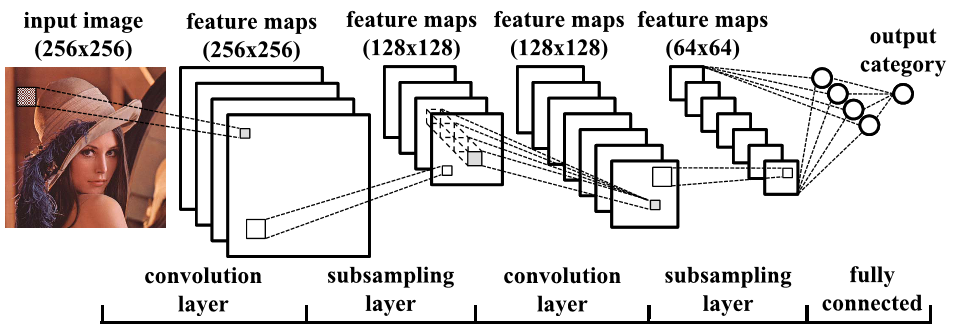
\includegraphics[width=1.0\linewidth]{figures/cnn_structure.png}
	\caption[Structure of a CNN]{Example of a simplified CNN structure with two convolutional layers for image classification. (Based on \parencite[p. 2284]{lecun_conv})} \label{fig:cnn-structure}
\end{figure}

The window mentioned before is called \textit{kernel} and holds the randomly initialized parameters that the network can learn. The kernel acts as a filter that is applied to each location in regular steps. In the two dimensional case, the kernel has a specified width and height, denoted as the \textit{kernel size}. Several kernels are used to extract multiple feature maps in each convolutional layer, but each output feature map is computed with its own kernel. This number of kernels is specified with its \textit{kernel depth}. Furthermore, the range the filter is moved in each dimension per step is called \textit{stride} \parencite{conv_guide}.

Each convolutional layer is usually followed by a non-linear activation function, preferably a rectifier. The reason is that the convolution is an affine transformation and is therefore linear. Stacking multiple linear operations could be mathematically reduced to a single one. Optionally, an additional \textit{pooling layer} can be applied that performs a subsampling onto the feature maps. Several pooling variants exist, while \textit{max pooling} is probably the most frequently used of them. It allows the representation to become roughly invariant to small rotations or translations of the input by only using the maximum value \parencite[p. 343]{deep_learning}.


\subsection{Convolution Operation} \label{sec:conv-op}

Generally speaking, a convolution in a mathematical operation on two functions $f(x)$ and $g(x)$. Its operator is typically denoted with an asterisk \parencite[p. 332]{deep_learning} and is defined as:

\begin{equation} \label{eq:conv-general}
  \big(f \ast g\big)(x) = \int f(\tau) \cdot g(x-\tau) \, d\tau .
\end{equation}

In terminology of convolutional networks, the function $f$ is termed as the \textit{input} and the filter $g$ is referred to as the \textit{kernel}. Moreover, the output of $ (f \ast g)(x) $ is called a \textit{feature map}.

As we are mainly dealing with discrete 2D images in this thesis, the formulation of equation \ref{eq:conv-general} can be discretized and reformulated as:

\begin{equation} \label{eq:conv-2d}
  \big(\textbf{I} \ast \textbf{K}\big)(x,y) = \sum\limits_{r=1}^{h} \sum\limits_{c=1}^{w} \textbf{I}_{c,r} \cdot \textbf{K}_{x-c,y-r} ,
\end{equation}

with an input $ \textbf{I} $ of size $w \times h$ and a two-dimensional kernel $ \textbf{K} $. Depending on the width and height of the kernel with a windows size of $ k \times k $ and the chosen stride $ s $, the shape of the convolved output changes. This is why the input is often enriched with zeros in order to have more control regarding the resulting output size. Surrounding the data with zeros is also known as \textit{zero-padding}. The use of no padding ($p=0$) is also called \textit{valid padding}, as depicted in Figure \ref{fig:conv_valid}. Also, when a padding of $p=\floor{k/2}$ is used that is half the kernel size, it is referred to as \textit{same padding}, shown in Figure \ref{fig:conv_same}. The reasons for its name is caused by the fact that the input and output size stay unchanged when a stride of $ s=1 $ is used.

\begin{figure}[htpb]
\centering
\begin{subfigure}{0.5\textwidth}
  \centering
  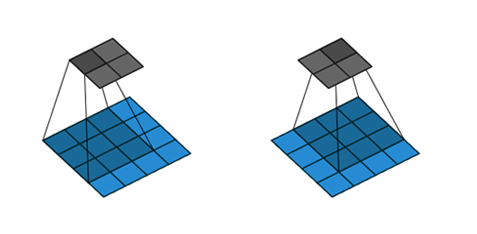
\includegraphics[width=.9\linewidth]{figures/conv_valid.png}
  \caption{$p=0$ (valid), $s=1$}
  \label{fig:conv_valid}
\end{subfigure}%
\begin{subfigure}{0.5\textwidth}
  \centering
  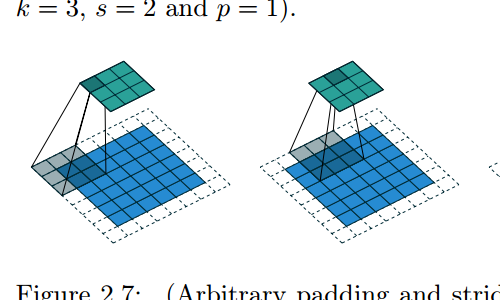
\includegraphics[width=0.9\linewidth]{figures/conv_same.png}
  \caption{$p=1$ (same), $s=2$}
  \label{fig:conv_same}
\end{subfigure}
\caption[Convolution Operation]{Visualizations of the convolutional operation with an $3 \times 3$ kernel but different settings for padding and stride. The white squares in (b) represent the padded zeros. (From \parencite{conv_guide})}
\label{fig:conv}
\end{figure}

It must be noted that the size of the kernel, padding and stride does not necessarily have to be equal in each dimension. But nevertheless, this is often the case in many practical applications.

\subsection{Transposed Convolution Operation}

The application of the previously presented convolution operation usually transforms the input into lower-dimensional feature maps. However, there are use cases where we would like to go the other way round, while keeping the connectivity pattern of a convolution. One application example is a convolutional autoencoder which is explained in further detail in Section \ref{sec:autoencoder}. This operation is referred to as \textit{transposed convolution}\footnote{Mistakenly, the transposed convolution is often called \textit{deconvolution}. But because it is not actually performing the reverse effect of a convolution, which is meant by the mathematical term of a deconvolution, it is strongly discouraged to name it so. An alternative name that is also often used is \textit{upconvolution}.}, which exchanges the forward and backward passes of a normal convolution. It is also called \textit{fractionally strided convolution}, because it can be emulated with a direct convolution using a zero-spaced input \parencite[p. 19]{conv_guide}. Such an implementation is less efficient, but it supports the intuition of how the resulting output shape looks like. Figure \ref{fig:conv_tp} shows an example of a transposed convolution.

\begin{figure}[htpb]
	\centering
	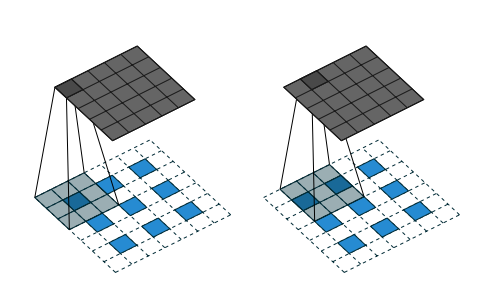
\includegraphics[scale=0.4]{figures/conv_tp.png}
	\caption[Transposed Convolution Operation]{Transposition of convolving an $6 \times 6$ input using a $3 \times 3$ kernel using $p=1$ and $s=2$. This is equivalent to performing a convolution using a zero-spaced $3 \times 3$ input with $p=1$ and $s=1$. (From \parencite{conv_guide})} \label{fig:conv_tp}
\end{figure}


\subsection{Advantages}

The three cenral design ideas are emphasized here to sum up the benefits of a convolutional network. It refers to \textit{sparse connections}, \textit{parameter sharing} and \textit{equivariance to translation} \parencite[p. 336ff.]{deep_learning}. The detailed advantages of these concepts are described in the following sections.

\subsubsection*{Sparse Connections}
The kernel size used in a convolution is smaller than the input. Consequently, less parameters have to be stored, as well as it can take advantage of local relationships present in the data. This also leads to a higher training efficiency and a radical reduction of memory requirements.

\subsubsection*{Parameter Sharing}
To handle all regions of the input data in the same manner, the parameters are \textit{reused} at every location as well. This is implemented by making use of only a single kernel which holds all learnable parameters.  Additionally, this \textit{weights sharing} decreases the number of parameters even further. To that end, Figure \ref{fig:conv_vs_fc} compares the connection pattern  and the sharing of model parameters of fully-connected layers against the convolutional case.

\begin{figure}[htpb]
\centering
\begin{subfigure}{0.5\textwidth}
  \centering
  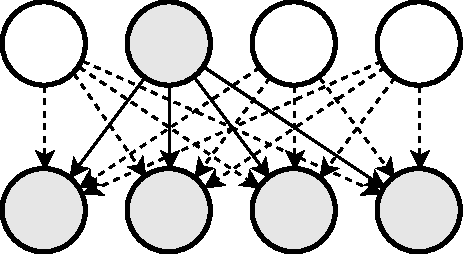
\includegraphics[width=.8\linewidth]{figures/fc2.pdf}
  \caption{}
  \label{fig:conv_vs_fc_fc}
\end{subfigure}%
\begin{subfigure}{0.5\textwidth}
  \centering
  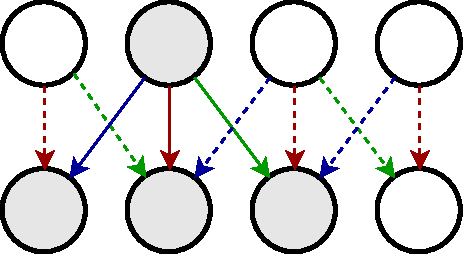
\includegraphics[width=0.8\linewidth]{figures/param_share.pdf}
  \caption{}
  \label{fig:conv_vs_fc_conv}
\end{subfigure}
\caption[Sparse Connections and Parameter Sharing in CNNs]{Comparison of the connection pattern and usage of parameters between (a) fully-connected layers and (b) convolutional layers. The use of the same color for interconnections denotes the sharing of parameters.}
\label{fig:conv_vs_fc}
\end{figure}

\subsubsection*{Equivariance to Translation}
The sharing of parameters leads to the third advantage. Because the kernel and its parameters are reused at every position, the model learns the same representations at every position \parencite[p. 339]{deep_learning}. For example, if an input image is translated by a fixed number of pixels, the network would handle it in the exact same way.

Unfortunately, convolutions are not tolerant to other transformations from the ground up. But to counteract these, other techniques exist such as a subsequent pooling stage to enable a slight rotation invariance, as already introduced before.


\subsection{Fully-Convolutional Networks}

The complete use of convolutional layers implicates a fourth advantage over fully-connected layers. Since the kernel size in each layer is independent regarding its input, the overall network could be fed with data of different dimension. In contrary, this is not possible anymore as soon as a single FC-layer is used at inference because its fixed-sized weight matrix has to be applied to the entire input, not just to a local region. Nevertheless, this does not imply that no fully-connected layer can be used at all when training the network. Depending on the architecture, FC-layers can be used in those parts of the network that are only used during training, but not when a prediction is performed while inference. This advantage is taken into account for example when a \textit{deep convolutional generative adversarial network} (DCGAN)\footnote{Novel network training strategy for generative networks. A generator network $ G $ competes against a second discriminator network $ D $ in an alternating fashion. Further details in \parencite{gan}.} is trained, whose discriminator network is only used in training mode.

Regarding the problem of frame prediction that has to be solved within this thesis, it has to deal with a huge amount of data in every training iteration. Therefore, the advantages from this \textit{fully-convolutional network} (FCN) approach are taken into account and design the architecture in such a way that it is possible to train the neural network model on small image patches only. Afterwards, it is theoretically able to perform frame prediction on the whole image given a sequence of frames.


\section{Recurrent Neural Networks}

All previously presented network architectures suffer from one missing characteristic: their memory is kind of static and predictions are mostly based on the current inputs only. Consequently, they are hard to be applied on problems where data reveals some sequential or temporal properties. Two examples are handwriting recognition, were the understanding of previous words is required to deduce the current word's context. Also in our case, the knowledge of the past image frames is fundamental to be able to predict the future frames that naturally match to the given previous sequence. A framework that addresses this issue is a \textit{recurrent neural network} (RNN). In this section, we give an overview about their structure and formal description, as well as present a succession model that addresses its fundamental problems. It is to add that the whole section is mainly inspired by the great explanations in \parencite{understand_lstm}.


\subsection{Basics}

RNNs are a special class of neural networks that allows its models to form a directed cyclic graph. Thereby, they are able to hold a hidden state that represents the sequential dynamics of the past. Given an input sequence $ \textbf{X} = (\textbf{x}^{(1)}, \textbf{x}^{(2)},..., \textbf{x}^{(\tau)}) $, the $ \tau^{th} $ recurrent building block gets $\textbf{x}^{(\tau)}$ as its input of this sequence, as well as the hidden state $\textbf{h}^{(\tau-1)}$ of the previous one. These building blocks are typically referred to as a \textit{cell}. Because the first cell has no predecessor, its hidden state input $ \textbf{h}^{(0)} $ is usually manually fed with an zero-initialized state vector. Formally, an RNN can be described as follows:

\begin{equation} \label{eq:rnn}
\begin{aligned}
\textbf{h}^{(\tau)} &= \phi(\textbf{W}_{h} \textbf{h}^{(\tau-1)} + \textbf{W}_{x} \textbf{x}^{(\tau)} + \textbf{b}_1) \\
\textbf{y}^{(\tau)} &= \textbf{W}_{o} \textbf{h}^{(\tau)} + \textbf{b}_2
\end{aligned}
\end{equation}

where $ \textbf{W}_{h} \in \mathbb{R}^{d_h \times d_h} $ are the weights of the hidden-to-hidden transitions, $ \textbf{W}_{x} \in \mathbb{R}^{d_x \times d_h} $ the weights of the input-to-hidden connections, $ \textbf{W}_{o} \in \mathbb{R}^{d_h \times d_x} $ the weights of the hidden-to-output transitions and $ \textbf{b}_1, \textbf{h}^{(0)} \in \mathbb{R}^{d_h}$ as well as $\textbf{b}_2, \textbf{x}^{(\tau)}, \textbf{y}^{(\tau)} \in \mathbb{R}^{d_x} $ the biases, initial state, input and output respectively \parencite[p. 2]{rnn-batchnorm}, \parencite[p. 381]{deep_learning}. The activation function $ \phi(\textbf{z}) $ is usually chosen to be a hyperbolic tangent.

Like convolutional networks, RNNs take advantage of sharing parameters over different parts of the model \parencite[p. 374]{deep_learning}. But in this case, model parameters are shared over the temporal domain. This allows the network to generalize specific properties across the whole input sequence. Consequently, a model can extract patterns that can occur at any or even multiple positions within the sequence of data.

\subsubsection{Structure}

For a better understanding of how recurrent networks work, it is helpful to take a closer look on its graphical model that was formally described by equation \ref{eq:rnn}. As it can be seen in Figure \ref{fig:rnn-loop}, the hidden state transition can be compactly visualized using a loop. These loops represent the influence of the past values with respect to the current value. However, to have a representation that is analogous to the already shown model, it is possible to unroll the loop in order to convert it back to a valid DAG. The unrolled recurrent network is depicted in Figure \ref{fig:rnn-unrolled}.

\begin{figure}[htpb]
\centering
\begin{subfigure}{0.26\textwidth}
  \centering
  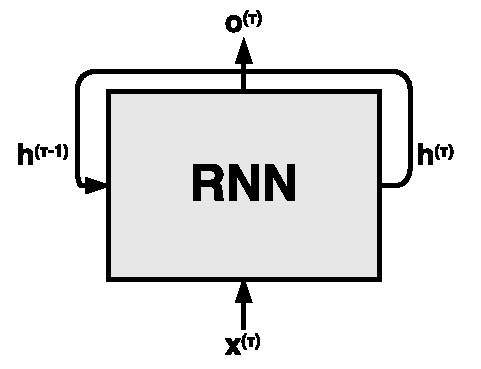
\includegraphics[scale=0.5]{figures/rnn_loop.pdf}
  \caption{}
  \label{fig:rnn-loop}
\end{subfigure}%
\begin{subfigure}{0.74\textwidth}
  \centering
  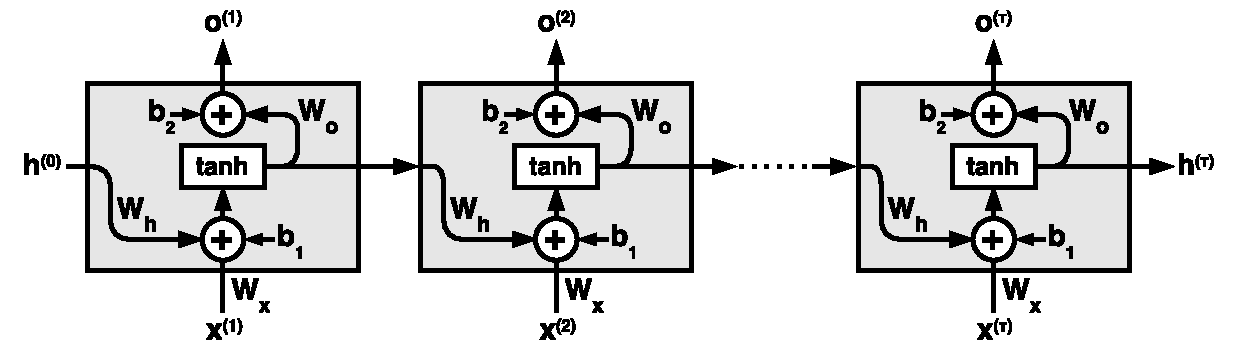
\includegraphics[scale=0.5]{figures/rnn_unrolled.pdf}
  \caption{}
  \label{fig:rnn-unrolled}
\end{subfigure}
\caption[Structure of Recurrent Cells]{Structure of recurrent network cells. The compact cyclic graph model in (a) can be unrolled to receive the model (b) that represents the network in form of an acyclic graph. (Based on \parencite{understand_lstm})}
\label{fig:rnn}
\end{figure}

In addition, the framework for recurrent models is very flexible as well. Depending on the implementation, it allows to process either a fixed or even a dynamic number of inputs. This property extends to the number of outputs as well. In contrary, convolutional or artificial neural networks require to define the input and output size at graph construction time. Further, they have to process all data in one chunk and do not allow to handle only single elements of the sequence one after the other. Some example input-output modes of recurrent networks are visualized in Figure \ref{fig:rnn-modes}.

\begin{figure}[htpb]
\centering
\begin{subfigure}{0.3\textwidth}
  \centering
  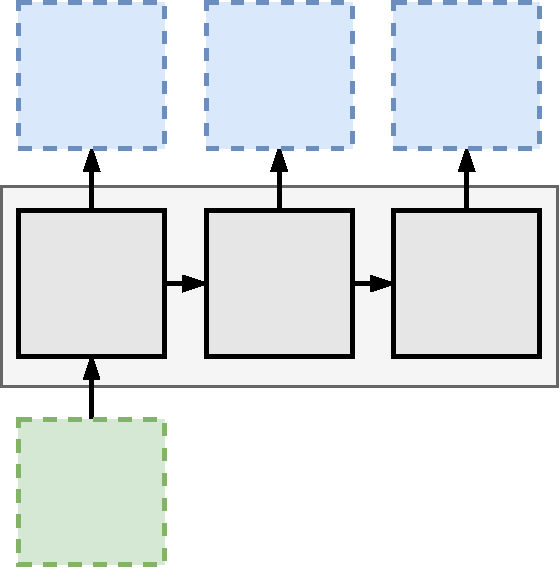
\includegraphics[width=.8\linewidth]{figures/one2many.pdf}
  \caption{}
  \label{fig:rnn-one2many}
\end{subfigure}%
\begin{subfigure}{0.3\textwidth}
  \centering
  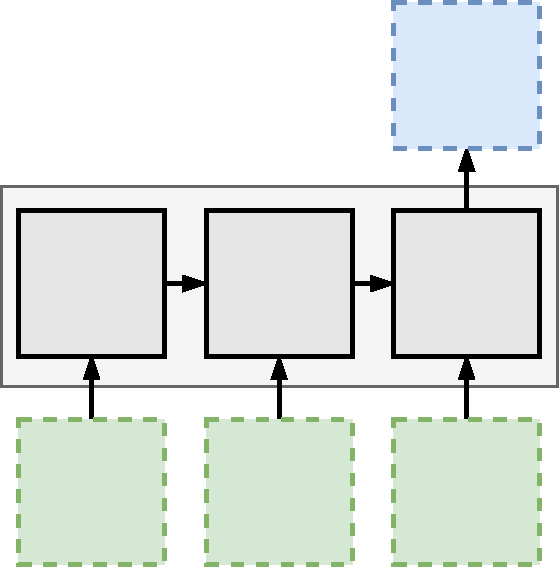
\includegraphics[width=.8\linewidth]{figures/many2one.pdf}
  \caption{}
  \label{fig:rnn-many2one}
\end{subfigure}
\begin{subfigure}{0.3\textwidth}
  \centering
  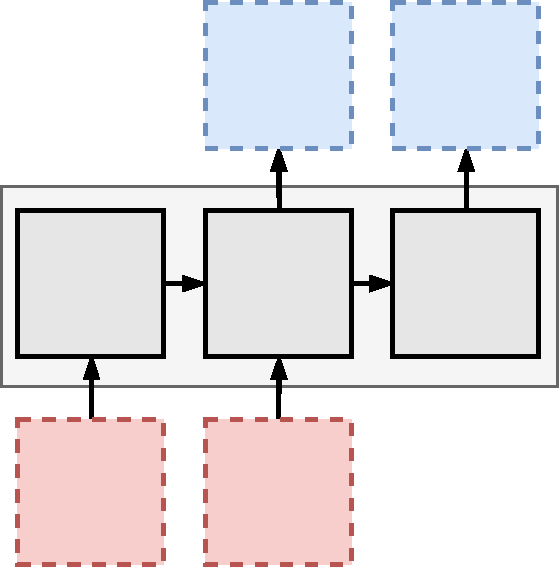
\includegraphics[width=.8\linewidth]{figures/many2many.pdf}
  \caption{}
  \label{fig:rnn-many2many}
\end{subfigure}
\caption[Examples of RNN Input-Output Modes]{Visualization of different recurrent network input-output modes: (a) one-to-many, (b) many-to-one, (c) many-to-many. Red squares denote the inputs, gray squares the recurrent cells and all outputs are colored in blue. Input and output squares can be understood as either further neural networks or the direct input and output. (Based on \parencite{rnn-effectiveness})}
\label{fig:rnn-modes}
\end{figure}

Besides the flexibility in the number of inputs and outputs, the recurrent components of the model is very adaptable as well. In common with the use of multiple neural network layers in order to achieve deeper and therefore more powerful models, several recurrent network layers can also be stacked on top of each other to enable a higher temporal depth. Various practical experiments, such as in \parencite{beyond_snippets_video_class}, \parencite{conv_lstm_nowcasting} or \parencite{unsup_learn_lstm}, have shown that \textit{multi-layer RNNs} are able to deliver better results compared to corresponding single-layer variants. Figure \ref{fig:rnn-multilayer} shows an example of a two-layer recurrent network. As a downside, the increase in the number of recurrent layers usually has a tremendous effect on the memory requirements and the network training time.


\begin{figure}[htpb]
\centering
\begin{subfigure}{0.3\textwidth}
  \centering
  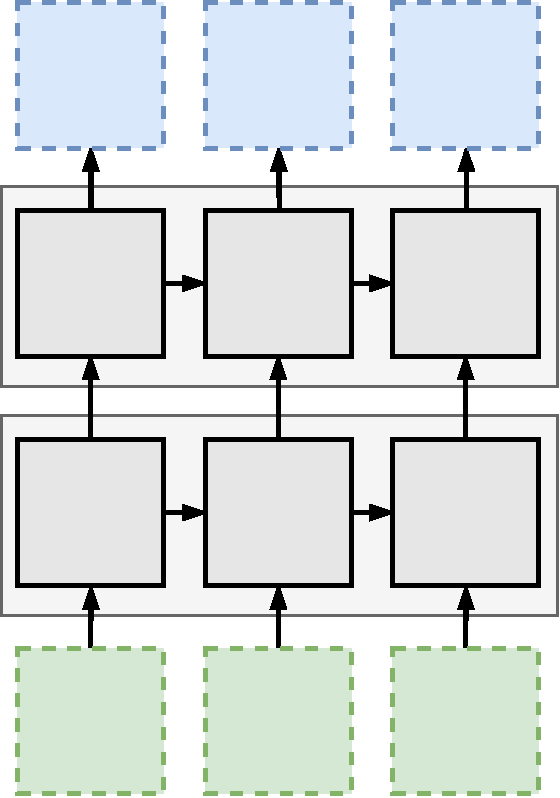
\includegraphics[width=.8\linewidth]{figures/rnn-multilayer.pdf}
  \caption{}
  \label{fig:rnn-multilayer}
\end{subfigure}%
\begin{subfigure}{0.3\textwidth}
  \centering
  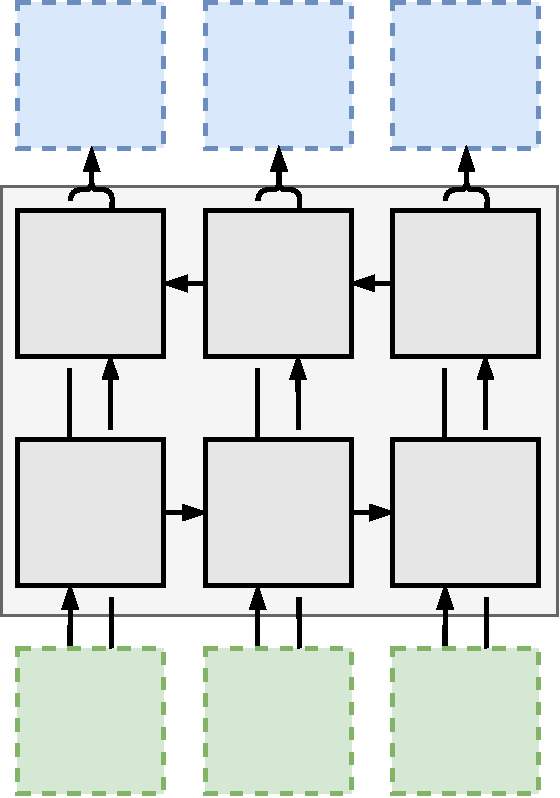
\includegraphics[width=.8\linewidth]{figures/rnn-bidirectional.pdf}
  \caption{}
  \label{fig:rnn-bidirectional}
\end{subfigure}
\caption[Deep Recurrent Network Architectures]{Examples of deeper recurrent network architectures. The figure in (a) shows a two-layer RNN, while (b) shows a single-layer BRNN. Both bidirectional outputs per cell of the latter model are combined and could be further processed by subsequent neural networks. (Based on \parencite{rnn-effectiveness})}
\label{fig:rnn-advanced}
\end{figure}

Additionally, the input sequence could be processed in both directions. This can be enabled by combining an RNN that starts at the beginning of the sequence with a second RNN starting from the very end backwards through time. In consequence, these so called \textit{bidirectional recurrent neural networks} (BRNN) are also able to have access to its future input information \parencite[p. 394ff.]{deep_learning}. It is to add that the recurrent weights are not shared in both directions. An example of such a bidirectional model is depicted in Figure \ref{fig:rnn-bidirectional}. The same idea could also be extended to a sequential processing of data in two dimensions, which is known as a \textit{grid RNN}.

\subsubsection{Backpropagation Through Time}

Analyzing the RNN structure might raise the question of how this effects the training procedure, because the gradient flows through recurrent cells multiple times while backpropagating the error. It is important to see that recurrent networks are still feed-forward networks with the extension to reuse the same weights expanded in time. Consequently, the error still has to be propagated backwards starting from the last time step $ \tau $ like in standard backpropagation. Depending on the length of the sequence and the computational resources, it can proceed until the very beginning, or truncate the view of interest by stopping at a given limit. Additionally, given the shared weights $ \textbf{w} $ of two timesteps $\tau $ and $ \tau+1 $, the weight constraint $ \textbf{w}^{(\tau)} = \textbf{w}^{(\tau+1)} $ must be met. Therefore, $ \nabla \textbf{w}^{(\tau)} = \nabla \textbf{w}^{(\tau+1)} $ has to be fulfilled as well. This can be realized by computing the gradients for both time steps independently, but use the average of the following sum:

\begin{equation} \label{eq:bptt}
	\frac{\partial \mathcal{L}}{\partial \textbf{w}^{(\tau)}} + \frac{\partial \mathcal{L}}{\partial \textbf{w}^{(\tau+1)}}
\end{equation}

when the final model parameter update is performed using the update rule \parencite{rnn-bptt}. This principle can be extended to the total sequence length that is considered by the recurrent network and is referred to as \textit{backpropagation through time} (BPTT).

\subsubsection{Drawbacks} \label{sec:rnn-drawbacks}

Keeping the previously explained weight constraints in mind, the recurrent network has to perform a lot of correlated updates of the same model parameters at once. This is actually bad for stochastic gradient descent, as it prefers uncorrelated parameters for the stability of the training. Especially when a sequence gets quite long, this can yield mathematical instability due to many multiplications using the same shared weights. On the one side, the gradients can grow exponentially and become infinite \parencite{lstm}. On the other side, the network could not learn anything because the gradients vanish. This issue is known as the \textit{vanishing and exploding gradient problem}. The lack of learning long-term dependencies in recurrent networks has been identified in \parencite{hochreiter} and \parencite{rnn-vanish}. Fortunately, other RNN variants exist that can deal with long-term dependencies. The currently most prominent version is introduced in the following section.


\subsection{Long Short-Term Memory}

Initially introduced by Hochreiter and Schmidhuber, the \textit{long short-term memory} (LSTM) became kind of the default recurrent network implementation as it is capable to deal with long range dependencies. Over the years, it has been revised by a couple of follow-up studies \parencite{lstm_peep} \parencite{lstm_v2} and is used in many practical applications today.

The central advancement of LSTMs over traditional recurrent networks is the so called \textit{memory cell state} $\textbf{C}^{(\tau)}$. While a simple RNN cell overrides its state at each time step, the LSTM's memory cell update exhibits only minor linear interaction, so that information could flow through very easily. Moreover, this simplifies the gradient flow backwards through time \parencite{rnn-batchnorm}. It follows that an LSTM cell inverts the core issue it tries to solve. Instead of learning to remember things, it is actually trained to learn what can be forgotten. In this way, keeping information over a longer period of time became its default setting.

To regulate the update of the internal memory state, the LSTM introduces the use of an attentive gating mechanism. At each time step, it is controlled by three trainable gates in order to accumulate or remove content from its state. Firstly, the \textit{input gate} determines the flow of information from the current input $ \textbf{x}^{(\tau)} $. Secondly, the \textit{forgot gate} regulates to which extend the information from the past cell state $\textbf{C}^{(\tau-1)}$ is kept. And lastly, the LSTM output state $\textbf{h}^{(\tau)}$ is specified by the filtered cell state using the \textit{output gate}. This mechanism allows constant error flow and enables to build a long-term understanding even when applied to long sequences. All this can be formalized as:

\begin{equation} \label{eq:lstm}
\begin{aligned}
\Spvek{\tilde{\textbf{f}}^{(\tau)}; \tilde{\textbf{i}}^{(\tau)}; \tilde{\textbf{o}}^{(\tau)}; \tilde{\textbf{c}}^{(\tau)}} &= \textbf{W}_{h} \, \textbf{h}^{(\tau-1)} + \textbf{W}_{x} \, \textbf{x}^{(\tau)} + \textbf{b} \\
\hat{\textbf{c}}^{(\tau)} &= tanh(\tilde{\textbf{c}}^{(\tau)}) \\
\textbf{C}^{(\tau)} &= \sigma(\tilde{\textbf{f}}^{(\tau)}) \odot \textbf{C}^{(\tau-1)} + \sigma(\tilde{\textbf{i}}^{(\tau)}) \odot \hat{\textbf{c}}^{(\tau)} \\
\textbf{h}^{(\tau)} &= \sigma(\tilde{\textbf{o}}^{(\tau)}) \odot tanh(\textbf{C}^{(\tau)})
\end{aligned} ,
\end{equation}

where $ \textbf{W}_h \in \mathbb{R}^{d_h \times 4d_h} $ are the shared weights for the hidden to hidden transitions at time step $ \tau $, $ \textbf{W}_x \in \mathbb{R}^{d_x \times 4d_h} $ the shared weights for the input to hidden connections, $ \textbf{b} \in \mathbb{R}^{4d_h} $ the biases, and $ \textbf{C}^{(0)}, \textbf{h}^{(0)} \in \mathbb{R}^{4d_h} $ the initial states of the memory cell and the hidden state, respectively \parencite{rnn-batchnorm}. The last dimension of the weight matrices and biases are multiples of four, because the matrices are concatenations of weights for all three gates plus the new candidate cell state $ \hat{\textbf{c}}^{(\tau)} $ for computational efficiency. The input, forget and output gates are labeled as $ \textbf{i}, \textbf{f} $ and $ \textbf{o} $. Furthermore, the operator $ \odot $ denotes the Hadamard product\footnote{The Hadamard product defines the entry-wise product of two matrices with the same dimension.} and a tilde indicates the term before the corresponding activation is applied, so that for example $ \textbf{f}^{(\tau)} = \sigma(\tilde{\textbf{f}}^{(\tau)}) $.


\subsubsection{Structure}

As depicted in Figure \ref{fig:lstm}, the internal structure of an LSTM cell looks way more complex compared to the simple RNN of Figure \ref{fig:rnn-unrolled}. Nevertheless, the role of each single building block has actually a quite simple interpretation.

\begin{figure}[htpb]
	\centering
	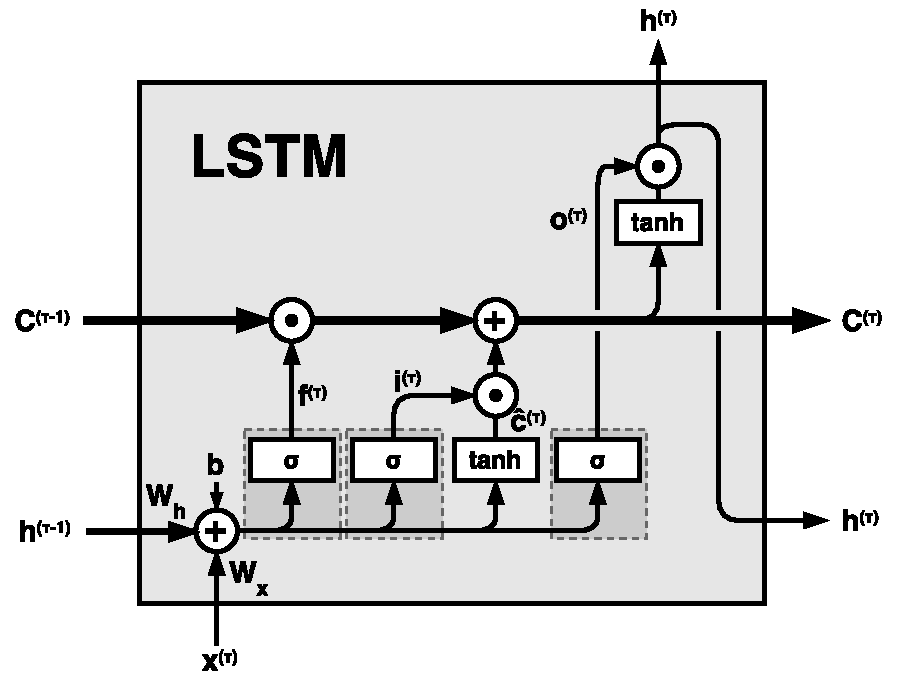
\includegraphics[width=.8\linewidth]{figures/lstm.pdf}
	\caption[Structure of a LSLTM Cell]{Structure of a LSTM cell. The flow of the cell state is highlighted in bold. Gated unites are emphasized with a dotted box. (Based on \parencite{understand_lstm})} \label{fig:lstm}
\end{figure}

As stated before, the fundamental enhancement of LSTMs is the cell state $\textbf{C}^{(\tau)}$, denoted as a bold line in the graphic. From its previous cell state to the next, there are just two interaction points where its content gets manipulated. First, using a pointwise multiplication with the output of the forget gate $\textbf{f}^{(\tau)}$, a specific part of the previous state can be partly or fully deleted. Afterwards, the new candidate cell state $ \hat{\textbf{c}}^{(\tau)} $ is added to it, which is only regulated by the input gate $ \textbf{i}^{(\tau)} $. The third gate $ \textbf{o}^{(\tau)} $ has no effect on the cell state itself and governs the hidden output only.
The interpretation of how each single gated unit works is the following: each gate itself is a fully-connected neural network layer, that receives the weighted sums of the input $\textbf{x}^{(\tau)}$ and the previous hidden state $\textbf{h}^{(\tau-1)}$ as its input. That is the reason why they are also often referred to as \textit{FC-LSTM}. Additionlly, as it can be seen in Figure \ref{fig:lstm}, every gate uses a sigmoid as its activation function that is followed by an Hadamard product. Consequently, the output of any gate is in range $ [0, 1] \in \mathbb{R}^{d_h \times 4d_h} $, where a value of one means let the whole information flow through, while zero intends to forget everything. 

\subsubsection{Variants}

The long short-term memory belongs to the family of \textit{gated RNNs} \parencite[p. 411]{deep_learning}. Since its invention, a couple of related implementations have been introduced. One example extends the LSTM by having so called \textit{peephole connections}, proposed in \parencite{lstm_peep}. These additional connections have the purpose that each gating unit has a direct access to the previous memory cell state $ \textbf{C}^{(\tau-1)} $. The motivation for this is to allow the units to learn when to open or close their gates based on the cell state \parencite{lstm-space}, in order to learn more precise timings.

Another example is the \textit{gated recurrent unit} (GRU) \parencite{gru}, which also regulates the flow of information comparable to an LSTM, but without having a separate memory cell. Additionally, its gates for input and output are merged to a single \textit{update gate}, which leads to a similar performance but with a lower memory footprint \parencite{gru-video}. The forgot gate in context of a GRU is typically called \textit{reset gate}.

A further, novel variant of LSTMs will be presented in Chapter \ref{chapter:implementation}, which is inspired by the strengths of convolutional neural networks. Aside from that, it will formalize the use of peephole connections as well.


\section{Encoder-Decoder Networks}

In order to learn useful representations, the generic, informative content has to be extract from the given data. But in many cases, we have to deal with a tradeoff between obtaining valuable properties and preserving as much information as possible regarding the inputs. Additionally, intense overfitting effects have to be handled when these representations are learned in a supervised fashion, because an acceptable amount of training data is often not on-hand for this purpose \parencite[p. 527]{deep_learning}. Therefore, this section focuses on concepts that are able to end up with good representations on the basis of unlabeled data in an \textit{unsupervised learning} process. 


\subsection{Autoencoders} \label{sec:autoencoder}

An \textit{autoencoder} is a commonly known neural network model that is able to reconstruct its own input. It consists of two components that are usually arranged in a mirrored style. First, an \textit{encoder} $ f(\textbf{x}) = \textbf{z} $ that maps any given input $ \textbf{x} \in \mathbb{R}^{d_x} $ to its internal representation $ \textbf{z} \in \mathbb{R}^{d_z} $. Second, a \textit{decoder} function $ g(\textbf{z}) = \textbf{x}^\prime $ that is able to map the representation back to its input. Due to the analogy to encoding and decoding, the learned representation is also often referred to as \textit{code}. In addition, the input and output layer of such networks have the same number of nodes. A simplified autoencoder model is visualized in Figure \ref{fig:autoencoder}. 

\begin{figure}[htpb]
	\centering
	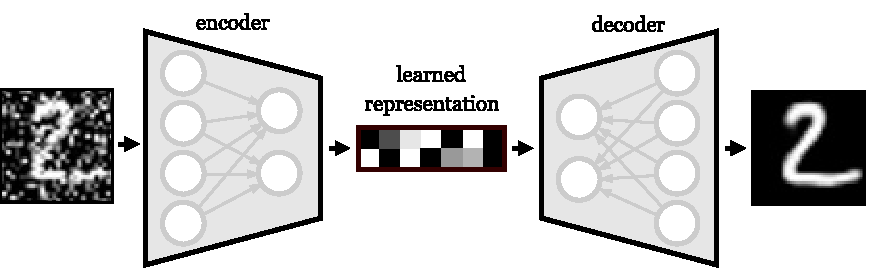
\includegraphics[width=.8\linewidth]{figures/encoder_decoder.pdf}
	\caption[Structure of an Autoencoder]{Simplified structure of a denoising autoencoder in an undercomplete setting to reconstruct images of handwritten numbers from the MNIST dataset.} \label{fig:autoencoder}
\end{figure}

The encoder and decoder components can be of any kind. In the simplest case, a neural network with only one single hidden layer could be used. However, it has been shown that deeper networks are able to yield better representations compared to shallow variants \parencite{autoenc_deeper}. Furthermore, the use of convolutional layers is usually preferred for image processing tasks, referred to as \textit{convolutional autoencoders}.

Reconstructing the input might sound trivial in first place. And honestly, the model itself that is able to learn the identity mapping $ g(f(\textbf{x})) = \textbf{x} $ and especially its output is not very interesting, since the network would just perform a copy operation. Instead, we are more interested in some special properties of the latent variable $ z $. These can be provoked by restricting the encoder, decoder or input with some additional constraints so that the model is not able to perform a perfect copy. Moreover, the dimensionality of the internal representation could be varied in order to force the model that it learns to prioritize which fraction of the input is worth to have in contemplation. Hence, it learns valuable properties regarding the data, which might even be useful to cope with other related tasks. Autoencoder models received increasing attention in recent years, especially in relation with \textit{generative models} \parencite[p. 502]{deep_learning}.

\subsubsection*{Undercomplete Autoencoders}

On the one side, in the typical \textit{undercomplete} case where the dimensionality of the representation is smaller than the input and output, so that $ d_z < d_x $, a model can be trained to reconstruct the original data \parencite[p. 503]{deep_learning}. As an application example, this can yield in an image compression algorithm, where the encoder compresses an input image to another representation of lower size. Afterwards, the decoder network can be used to recover the image data. As a result, depending on how much lower the size of the representation and the dissimilarity of the reconstruction compared to its original image is, the better is our learned representation. It then would have learned to preserve the image information in a more compact way.

\subsubsection*{Regularized Autoencoders}

On the other side, there are also use cases for \textit{overcomplete} models where the representation's dimensionality could exhibit an equal or even higher dimension than the input and output\footnote{It is to be added that the presented regularization strategies can also be used for undercomplete autoencoders.}, so that $ d_z \geq d_x $. But this requires to apply regularization techniques in order to learn useful features. The reason is that such a high model capacity can easily end up in overfitting \parencite[p. 504f.]{deep_learning}. One first possibility is to extend the loss function with an additional sparsity penalty, so that the \textit{sparse autoencoder} network tries to minimize:

\begin{equation} \label{eq:autoenc-sparse}
	\mathcal{L}(\textbf{x}, g(f(\textbf{x}))) + \lambda \cdot \Omega(\textbf{z}) ,
\end{equation}

where $ \lambda $ controls the tradeoff between sparsity and reconstruction and regularizer term $ \Omega(\textbf{z}) $ can be any valid loss function, such as $ \ell_2 $. This sparsity constraint reduces the autoencoder's degrees of freedom and therefore prevents overfitting. To put it another way, the model is virtually undercomplete by having a compactly distributed representation instead of a lower dimensionality. Alternatively, sparsity could also be achieved by only using the $ k $ most meaningful activations in a \textit{k-sparse autoencoder} by zeroing out weak hidden units manually \parencite{k-sparse-autoenc} or by using rectifier units in the last encoding layer \parencite{rect-autoenc}.

A second regularization strategy is to modify the reconstruction term of the loss function itself by adding random noise to the input. These networks are called \textit{denoising autoencoders} and have to learn how to correct back the added noise for the purpose of reconstructing the original noise-free image \parencite[p. 507]{deep_learning}. Therefore, the network has to learn a deeper understanding of the input data instead of simply copying its content. As a consequence, it has to minimize:

\begin{equation} \label{eq:autoenc-denoise}
	\mathcal{L}(\textbf{x}, g(f(\tilde{\textbf{x}}))) ,
\end{equation}

where $ \tilde{x} $ is the randomly corrupted version of the ground truth input $ x $.


\subsection{Recurrent Encoder-Decoder Models} \label{sec:rnn_enc_dec}

The general idea of the encoder-decoder framework can also be applied to recurrent networks. Thus, it can build a complex representation by incorporating a whole sequence of inputs. To our knowledge, the \textit{recurrent encoder-decoder} model has been firstly introduced independently from each other in \parencite{brnn_fist} and \parencite{brnn_second}. Further, it has been used in  \parencite{unsup_learn_lstm}\footnote{The authors call this recurrent framework the \textit{LSTM autoencoder model} within their publication. But due to the fact that it can be generalized to another recurrent cell implementations, as well as it could be applied in a non-autoencoder fashion, the more general name \textit{recurrent encoder-decoder} model is used here as well. This name is also used in several follow-up works.} for the first time in context of image processing. But since then, it has been applied in numerous subsequent works \parencite{rnn-enc-dec1}, \parencite{rnn-enc-dec2}. Figure \ref{fig:rnn-autoencoder} shows an example of such a model in context of a recurrent autoencoder.

\begin{figure}[htpb]
	\centering
	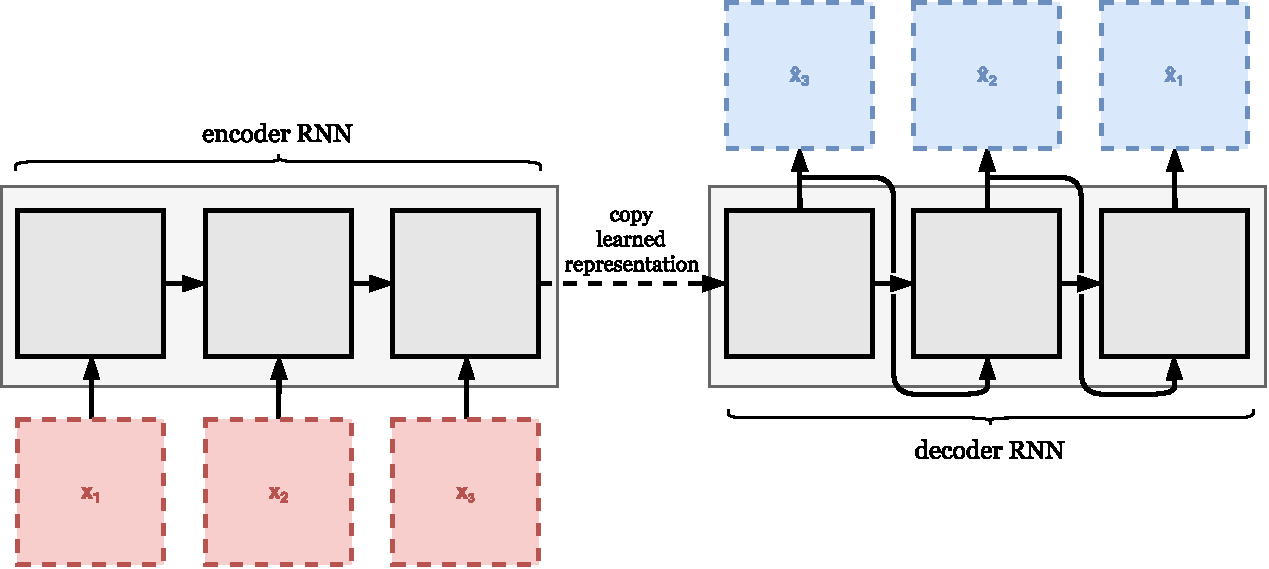
\includegraphics[width=.9\linewidth]{figures/rnn_autoencoder.pdf}
	\caption[Recurrent Autoencoder Model]{Basic structure of a conditional recurrent autoencoder. The inputs (red) are processed by the encoder RNN to learn the representation of the data in sequence. Then, the decoder RNN takes over to infer the reconstructions (blue) of the inputs in reverse order. (Based on \parencite{unsup_learn_lstm})} \label{fig:rnn-autoencoder}
\end{figure}

The encoder RNN builds the representation based on all inputs of the sequence and therefore takes advantage of its temporal or ordinal structure. Afterwards, the learned representation is used to initialize the hidden state $ \textbf{h}_{\textrm{dec}}^{(0)} $ of the decoder, in opposite to the otherwise customary zero initialization. The decoder RNN takes then over and outputs the prediction of the target sequence. Obviously, both the encoder and decoder recurrent networks could be extended to consist of multiple layers or bidirectional connections as well.

There are at least two possibilities of how the decoder can be designed. Firstly, an unconditional setting where each recurrent cell does \textit{not} receive the previous output as its input. Secondly, a conditional setting in which this additional connection from the cell's output to the input of the next element is present. Both have its reasons for and against. On the one side, it can be argued that conditioning on the previous output enables to learn more dynamics in the target sequence distribution. This conditioning might not be required in an autoencoder setting, where there is only exactly one ground truth target sequence. But when this architecture is applied to continue a series of frames in the future, it could be crucial to have access to the previous output. As an example, consider the prediction of a series of frames from a simple video game, where the player could walk either left or right in a specific situation. To properly predict the next outputs afterwards, it is fundamental to know which decision this particular recurrent cell has made. Otherwise, the RNN might end up in averaging over all possible outcomes. On the other side, it could also be argued that conditioning on the previous frame would end up in preventing the network to look deeper inside the encoder network \parencite{unsup_learn_lstm}.


\section{Batch Normalization}

Training a deep neural network model is said to be very hard. One reason for this is that every layer has not just to learn the overall representation directly from the beginning of the training, but also has to master the continuous change in distribution of its inputs, given all preceding layers. As an example, consider one layer in the middle of a deep network. At training time, its adjustments to the model parameters depend on its inputs, which is equivalent to the output of the previous layer. But the fact that the previous layer learns and modifies its weights and biases, it follows that the input to the following layer can change over time significantly. Especially at the very beginning of the training, due to the common use of random initialization. This ongoing change in the feature's distribution during training is known as the \textit{internal covariance shift} \parencite{rnn-batchnorm}.

One modern practice that tries to overcome this issue is called \textit{batch normalization} \parencite{batchnorm}. It performs a normalization on the inputs to a layer and transforms it to have a mean of zero and a standard deviation of one. Consequently, it compensates the covariate shift between two layers of the network. Its mathematical formulation is:

\begin{equation} \label{eq:bn}
\textrm{BN}(\textbf{x}; \gamma, \beta) = \beta + \gamma \frac{\textbf{x} - \mathbb{E}(\textbf{x})}{\sqrt{Var(\textbf{x}) + \epsilon}} ,
\end{equation}

where $ \textbf{x} \in \mathbb{R}^d $ is the output of the previous layer to be normalized, $\gamma \in \mathbb{R}^d $ and $\beta \in \mathbb{R}^d $ the learned shift and scale of the distribution, as well as $\epsilon \in \mathbb{R} $ that serves as a regularization parameter to avoid dividing by zero \parencite{rnn-batchnorm}.

When batch normalization is applied, two different modes during training and inference have to be considered. On the one hand at training time, batch normalization takes advantage of two simplifications, caused by the fact that full whitening of the inputs is very expensive. First, each feature dimension is normalized independently. Secondly, the statistics of $ \mathbb{E}(\textbf{x}) $ and $ Var(\textbf{x}) $ are estimated using the sample mean and sample variance based on each mini-batch of stochastic gradient training. On the other hand, the statistics have to be assessed using the entire training data during inference. One way to do so is to track the moving averaged mean and variance parameters of each batch-estimate while training the model, and finally use these averaged values when a prediction is performed. This is the way how batch normalization is used throughout this work.

The advantages of batch normalization are versatile:

\begin{itemize}
\item Compensation against internal covariate shift to achieve a stable distribution of activation values.
\item Separate normalization of individual feature dimensions, so that features are not decorrelated.
\item Speed-up training, because it allows to use higher learning rates.
\item Practice has shown that even a higher accuracy can be achieved compared to non-batch-normalized versions of a network model \parencite[p. 7]{batchnorm}.
\end{itemize}


\section{Image Similarity Assessment}

The practical use of deep learning in context of image generation tasks received a tremendous increase in recent years. Examples include denoising autoencoders (see Section \ref{sec:autoencoder}) for image reconstruction, semantic image completion \parencite{sem-img-inpainting}, the determination of optical flow \parencite{flownet}, \parencite{flow-static-img} or future  frame prediction of a given image sequence. The last mentioned field of application is in scope of this thesis. 

A neural networks main driver in respect to learning a good representation is the loss layer. Unfortunately, it found only little attention in most existing studies when applied in image processing tasks, at least until this year \parencite{loss-func-img-proc}. Therefore, this section provides an overview of the main challenges of image similarity assessment and introduces some approved methods, as well as novel approaches when training neural networks in context of pictures.


\subsection{Naive Approach}

The de facto standard loss function to compare a generated image with its ground truth target has been the \textit{pixel-wise squared error} (or $ \ell_{2} $) that was already mentioned in equation \ref{eq:mse}. It is easy to apply and usually provided by any neural network framework out-of-the-box. But as a downside, it suffers from some well-known limitations such as poor correlation with the human sense of perceptual quality \parencite{loss-func-img-proc}. The reason for this are twofold. First, $ \ell_{2} $ makes the assumption of a Gaussian noise model, which has its downsides when being applied to multimodal distributions. Second, it strongly penalizes outliers independently from local characteristics of the image, such as contrast or luminance. In contrary, the visual system of humans perceives noise in a different way.

\begin{figure}[htpb]
\centering
\begin{subfigure}{0.5\textwidth}
  \centering
  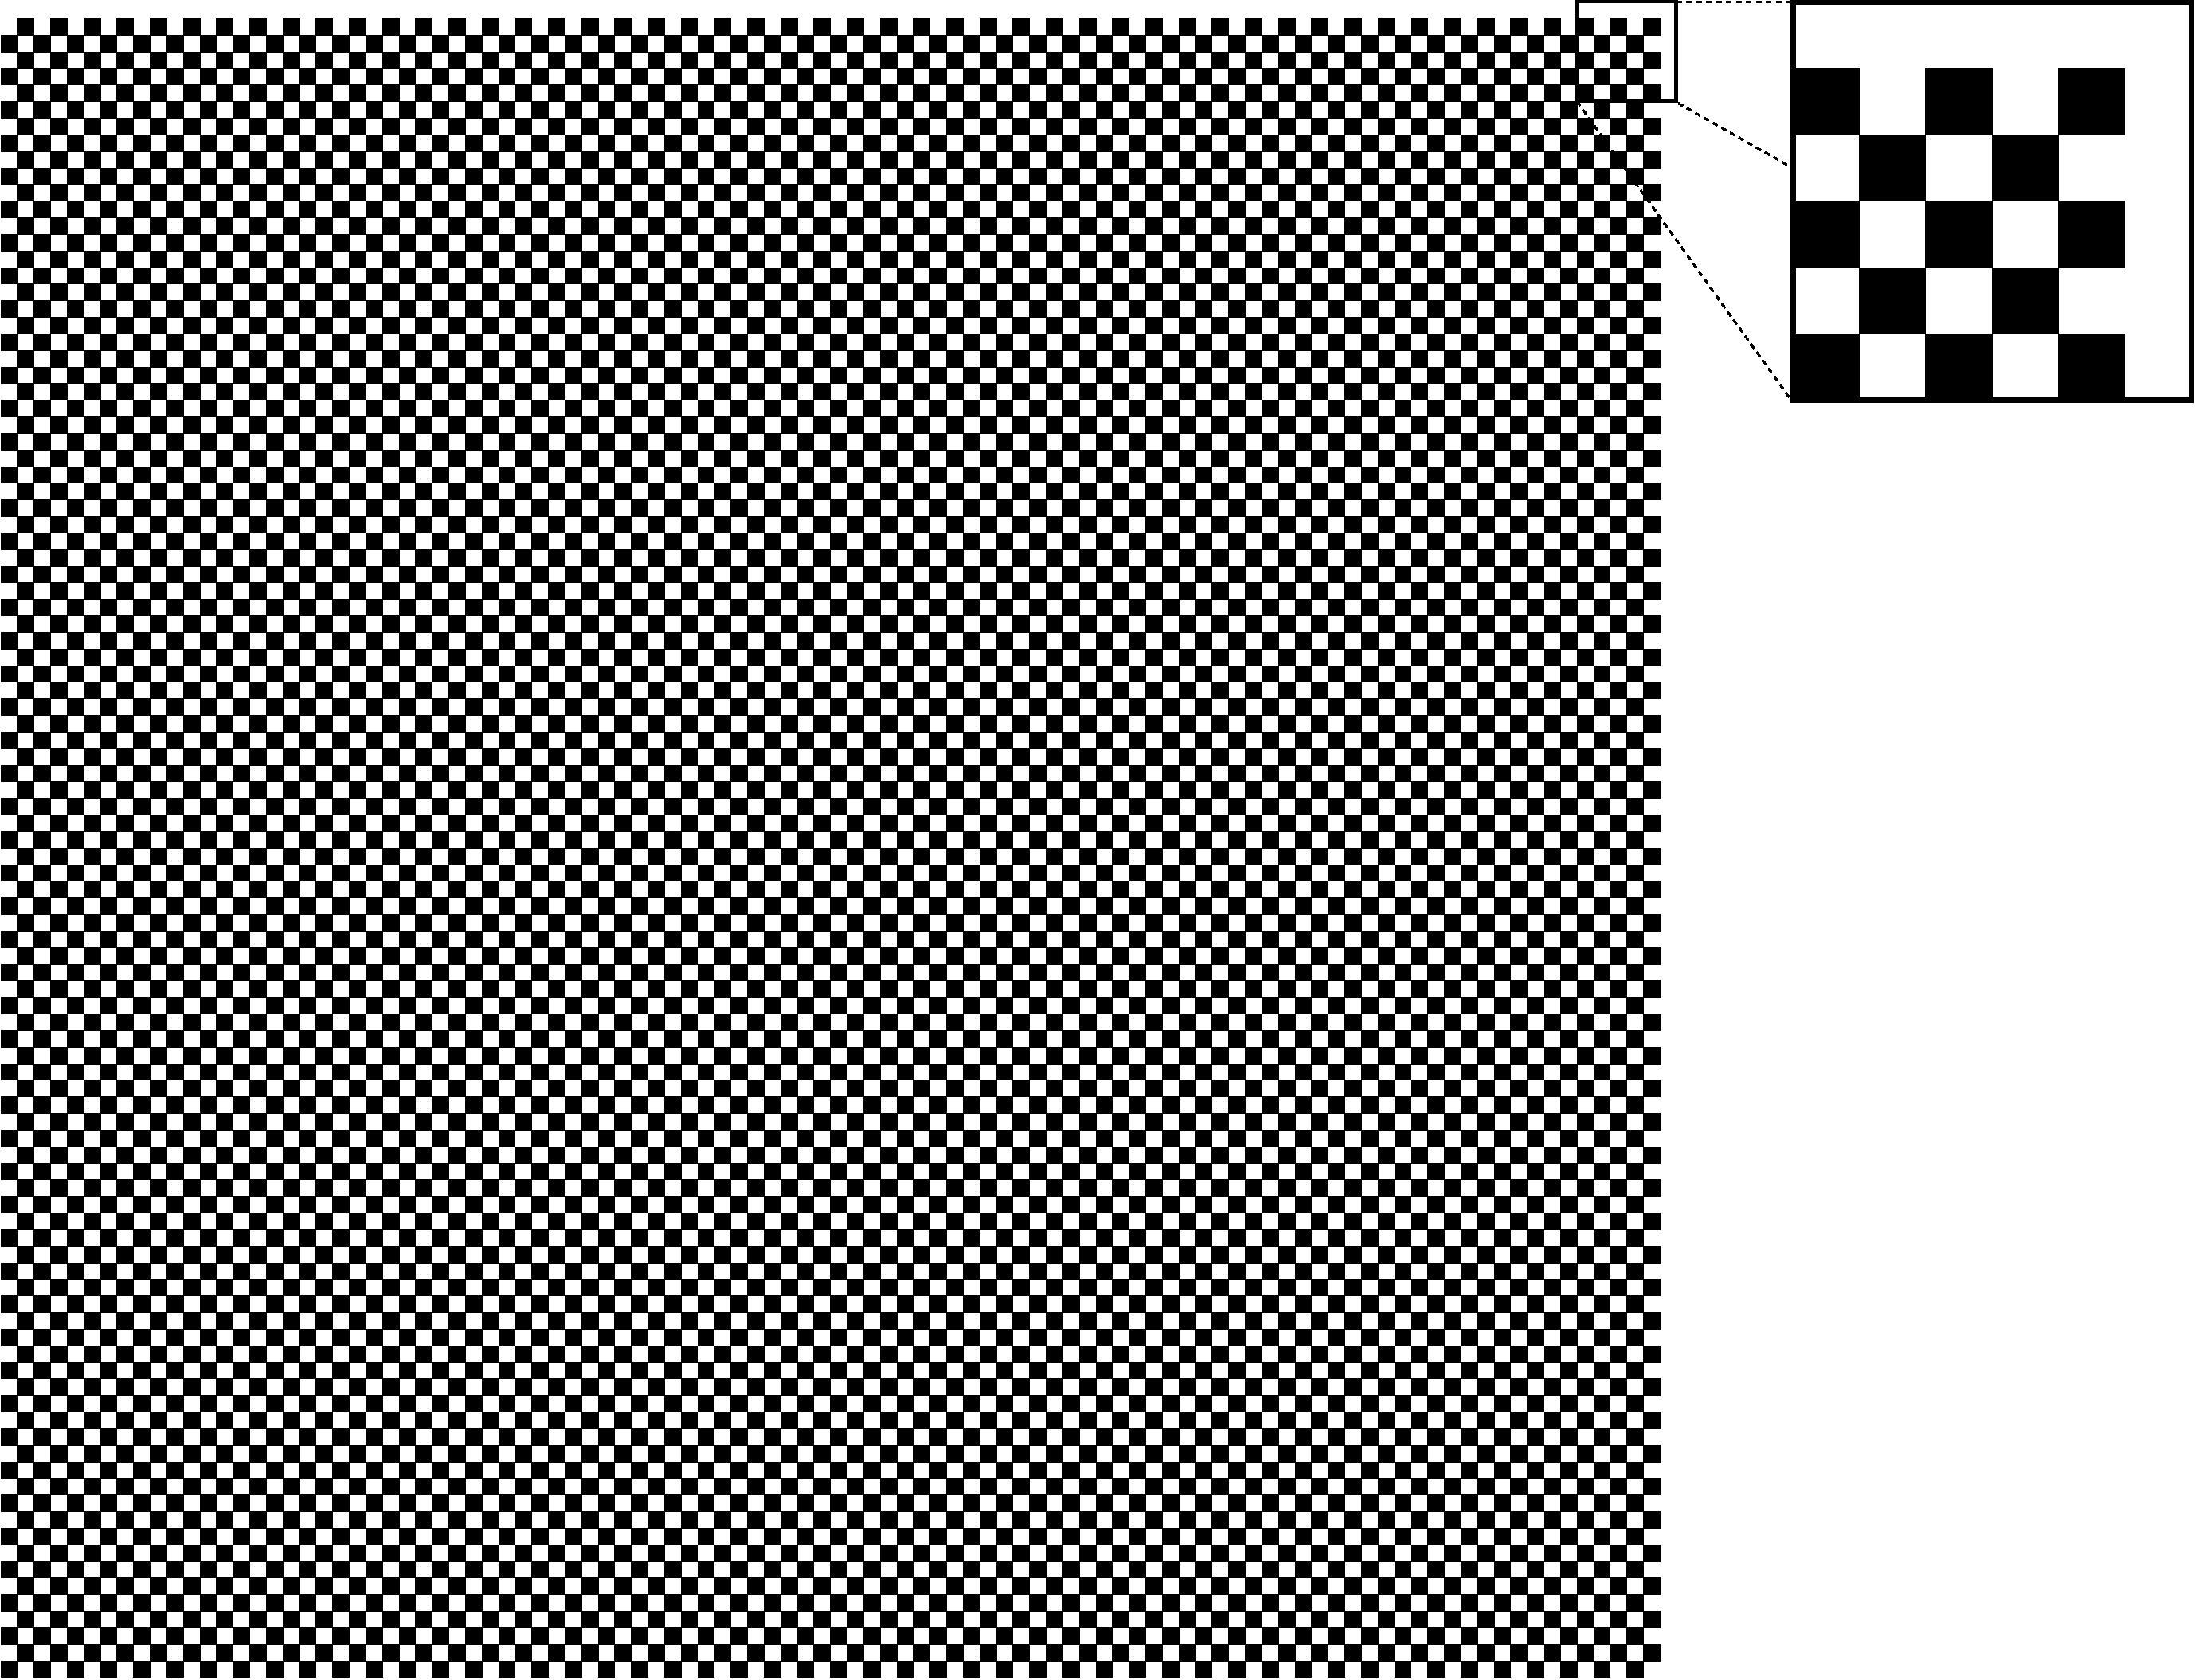
\includegraphics[width=.8\linewidth]{figures/chess1.pdf}
  \caption{}
  \label{fig:chess1}
\end{subfigure}%
\begin{subfigure}{0.5\textwidth}
  \centering
  
\includegraphics[width=.8\linewidth]{figures/chess2.pdf}
  \caption{}
  \label{fig:chess2}
\end{subfigure}
\caption[Example of $ \ell_{2} $ Weakness]{Example to demonstrate the weakness of $ \ell_{2} $ in context of perceptual image similarity.} \label{fig:chessfield}
\end{figure}

As an extreme but simple example, consider two images containing a chess field of black and white pixels as shown in Figure \ref{fig:chessfield}. From an aerial perspective, both images look completely identical, because it is perceived as a gray surface. Additionally, even when we look at it from a closer distance, we would still evaluate them as quite similar. This is for the very reason that both images provide the same colors, structure, sharpness or contrast. Unfortunately, assessing both images using the given squared error function results in the maximum possible difference. The reason for this is because it considers the squared differences of related pixels only. Even that this specific weakness is not solved by using the $ \ell_{1} $ loss, several studies have shown that the usage of the absolute error function slightly reduces the blur effect on edges in image generation processes of natural images \parencite{loss-func-img-proc} \parencite{deep_multiscale_video_pred}. Some example image reconstructions comparing the use of different loss functions are show in Figure \ref{fig:percept-vs-lp}.

\begin{figure}[htpb]
\centering
\begin{subfigure}{0.4\textwidth}
  \centering
  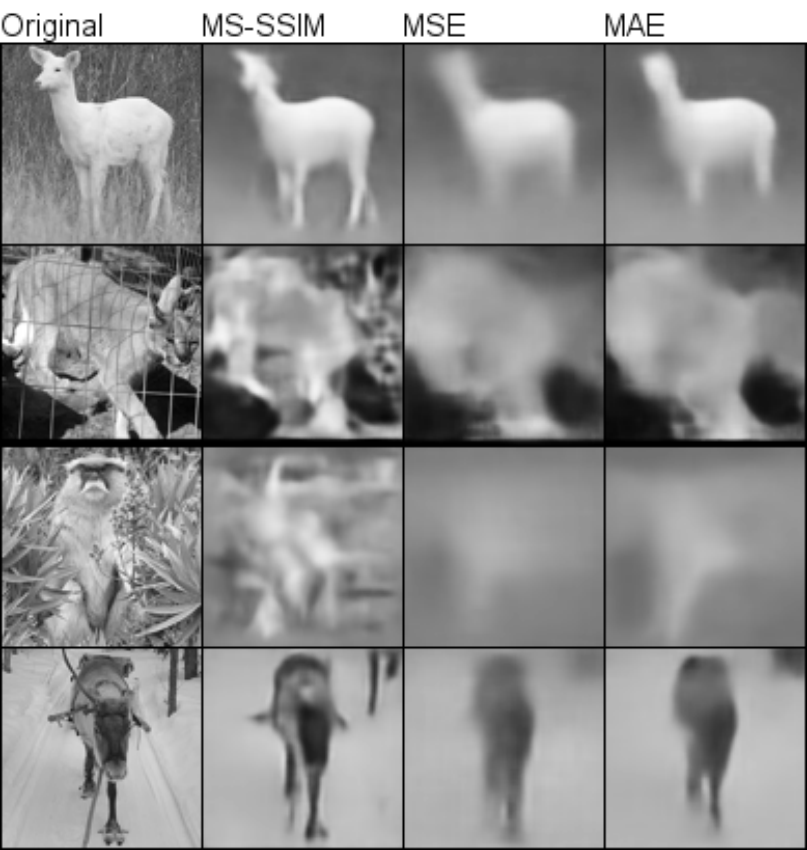
\includegraphics[width=.8\linewidth]{figures/img-loss-comp1.png}
  \caption{}
  \label{fig:percept-vs-lp1}
\end{subfigure}%
\begin{subfigure}{0.4\textwidth}
  \centering
  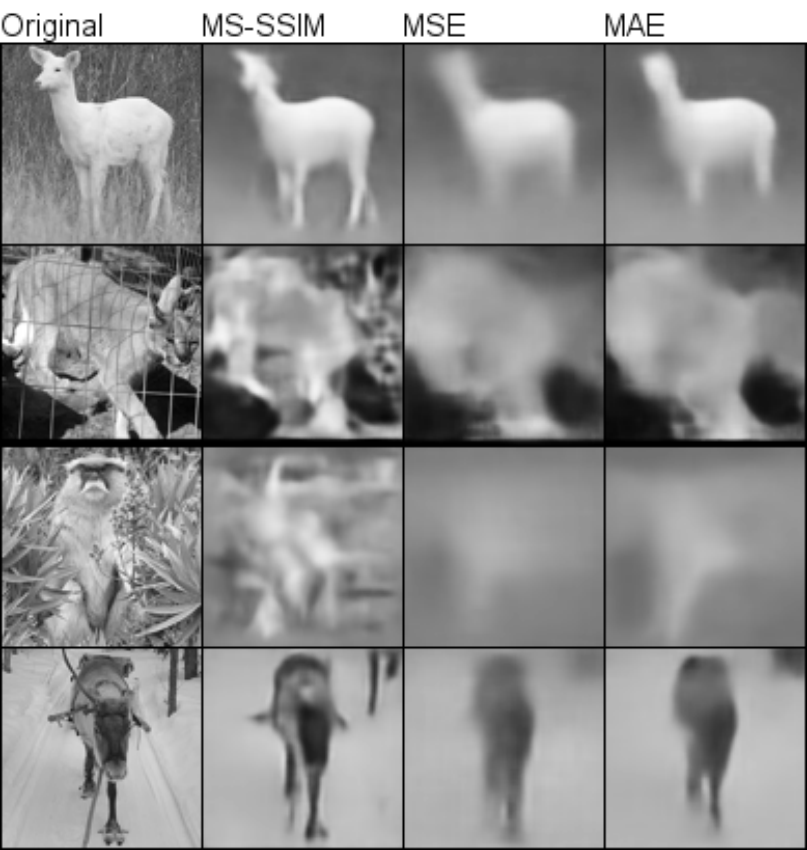
\includegraphics[width=.8\linewidth]{figures/img-loss-comp1.png}
  \caption{}
  \label{fig:percept-vs-lp2}
\end{subfigure}
\caption[Comparison of Reconstructions with Different Loss Functions]{Comparison of reconstructions with different loss functions using images from the STL-10 dataset: (a) where results using a perceptual motivated loss function were ranked first by human judgement, (b) where MAE or MSE were ranked best. (From \parencite{learning-perc-sim})}
\label{fig:percept-vs-lp}
\end{figure}


\subsection{Perceptual Quality Metrics}

The example in the previous section has shown that the consideration of the human visual perception is very important when assessing image similarity. With this in mind, a couple of metrics have been developed to evaluate image quality differences between two images. These metrics can be used either for a quantitative evaluation of generated results, or even as a loss function by doing some minor modifications to fulfill the required properties. Beside neural network training, these metrics have been originally invented to measure the quality of image compression codecs such as JPEG\footnote{JPEG: stands for \textit{Joint Photographic Experts Group} and is the name of the committee that created this compression standard for digital pictures.}.

In the following sections, $ \textbf{x} $ will denote the ground truth image and $ \textbf{y} $ its generated reconstruction to compare with.

\subsubsection*{Peak Signal-to-Noise Ratio}

A first metric to assess the similarity of generated images is the \textit{peak signal-to-noise ratio} (PSNR). It describes the ratio between the maximum possible image intensity and the corrupting noise that affects precision of the reconstruction. Its value is expressed in a logarithmic decibel scale, where a higher value indicates better quality. In terms of human perception, it is a rough approximation to evaluate reconstruction quality, because its denominator is still based on MSE. It is computed as follows:

\begin{equation} \label{eq:psnr}
\textrm{PSNR}(\textbf{x}, \textbf{y}) = 10 \cdot \log_{10} \Bigg( \frac{\textbf{y}_{max}^2}{\frac{1}{w \, h} \sum_{c=1}^{w} \sum_{r=1}^{h} (\textbf{x}_{c,r} - \textbf{y}_{c,r})^2 } \Bigg) ,
\end{equation}

where $ \textbf{y}_{max} $ is the maximum \textit{possible} intensity of any given image with size $ w \times h $.


\subsubsection*{Structual Similarity}

For predicting the perceived image quality, the \textit{structural similarity} (SSIM) index invented in \parencite{ssim} can be used as another assessment criteria. This full reference metric\footnote{Full reference metric (FR) is a quality term which means that the evaluation is based on every pixel of the entire ground truth image as a reference.} is an improvement over PSNR as it is based on several assumptions of the human vision system. Therefore, it assesses both images based on luminance $ l(\textbf{x}, \textbf{y}) $ , contrast $ c(\textbf{x}, \textbf{y}) $ and structural similarity $ s(\textbf{x}, \textbf{y}) $ \parencite{ms-ssim}. These components are defined as follows:

\begin{equation} \label{eq:ssim-components}
\begin{aligned}
l(\textbf{x}, \textbf{y}) &= \frac{2 \mu_x \mu_y + C_1}{\mu_x^2 + \mu_y^2 + C_1} \\
c(\textbf{x}, \textbf{y}) &= \frac{2 \sigma_x \sigma_y + C_2}{\sigma_x^2 + \sigma_y^2 + C_2} \\
s(\textbf{x}, \textbf{y}) &= \frac{2 \sigma_{xy} + C_3}{\sigma_x \sigma_y + C_3} ,
\end{aligned}
\end{equation}

where $ \mu_x $, $ \sigma_x $ and $ \sigma_{xy} $ is the mean, standard deviation and covariance of $ x $ and $ y $, respectively. Further, $ C_1 = (K_1 \cdot L)^2 $, $ C_2 = (K_2 \cdot L)^2 $ and $ C_3 = \frac{C_2}{2} $ are small constants for numerical stability, $K_1 = 0.01$ and $ K_2 = 0.03 $ by default and $ L=255 $ is the typical dynamic range of pixel-values for 8-bit \textit{gray-scale} images. These terms can be combined to define the SSIM index given by:

\begin{equation} \label{eq:ssim-combined}
\textrm{SSIM}(\textbf{x}, \textbf{y}) = \big[ l(\textbf{x}, \textbf{y})\big]^{\alpha} \cdot \big[c(\textbf{x}, \textbf{y}) \big]^{\beta} \cdot \big[ s(\textbf{x}, \textbf{y}) \big]^{\gamma} ,
\end{equation}

where $ \alpha $, $ \beta $ and $ \gamma $ parameterize the relative importance of all three components, typically $ \alpha = \beta = \gamma = 1 $. The terms for contrast and structure can be further simplified to $ cs(\textbf{x}, \textbf{y}) $ \parencite[p. 5]{loss-func-img-proc}, resulting in:

\begin{equation} \label{eq:ssim-simplified}
\begin{aligned}
\textrm{SSIM}(\textbf{x}, \textbf{y}) &= \frac{2 \mu_x \mu_y + C_1}{\mu_x^2 + \mu_y^2 + C_1} \cdot \frac{2 \sigma_{xy} + C_2}{\sigma_x^2 + \sigma_y^2 + C_2} \\
&= l(\textbf{x}, \textbf{y}) \cdot cs(\textbf{x}, \textbf{y}) .
\end{aligned}
\end{equation}

The SSIM index can be computed using a sliding window approach \parencite{ssim-slide}. Therefore, a square kernel\footnote{The initial paper states to use an $ 8 \times 8 $ window. But many open source libraries, and even the MATLAB implementation of the paper's author itself use a kernel size of $ 11 \times 11 $. In addition, some works list their evaluation results using several different kernel sizes.} of size $ 11 \times 11 $ and \textit{valid} padding is used that moves over the whole image, pixel by pixel. The index is then calculated in every local region and finally averaged to receive the overall image quality index for evaluation. The metric value is in range $ SSIM(\textbf{x}, \textbf{y}) \in [0, 1] $, where a higher value indicates more similarity.

\subsubsection*{Multi-Scale Structural Similarity}

Further studies have shown that the viewing conditions can have a tremendous influence on the perceived image similarity. Therefore, the SSIM index has been extended to incorporate the image on $ M $ different scales, where $ M=1 $ indicates the full-size image that is iteratively downsampled by a factor of two. This metric is known as the \textit{multi-scale structural similarity} (MS-SSIM) index for images \parencite{ms-ssim}. It is given by:

\begin{equation} \label{eq:ms-ssim}
\textrm{MS-SSIM}(\textbf{x}, \textbf{y}) = \big[ l_M(\textbf{x}, \textbf{y})\big]^{\alpha_M} \cdot \prod\limits_{j=1}^{M} \big[c_j(\textbf{x}, \textbf{y}) \big]^{\beta_j} \cdot \big[ s_j(\textbf{x}, \textbf{y}) \big]^{\gamma_j} ,
\end{equation}

where the exponents $ \alpha_M $, $ \beta_j $ and $ \gamma_j $ parameterize the relative importance of each component. The luminance difference $ l_M(\textbf{x}, \textbf{y}) $ is only computed for the smallest image size at scale $ M $. As a simple standard selection for the exponents, one can use $ \alpha_M = \beta_j = \gamma_j $ and $ \sum_{j=1}^{M} \gamma_j = 1 $. But by performing an empirical study in \parencite{ms-ssim}, the authors propose to use $ \beta_1 = \gamma_1 = 0.0448 $, $ \beta_2 = \gamma_2 = 0.2856 $, $ \beta_3 = \gamma_3 = 0.3001 $, $ \beta_4 = \gamma_4 = 0.2363 $ and $ \alpha_5 = \beta_5 = \gamma_5 = 0.1333 $ by incorporating $ M=5 $ scales. As a downside, evaluating multiple scales can be computational expensive. Additionally, the selected window size has to be smaller than the image at scale $ M $. Also, the image has to have an appropriate minimum size due to the iterative downsampling of the algorithm.


\subsubsection*{Sharpness Difference}

To quantitatively evaluate the difference in sharpness between two images, the \textit{sharpness difference} metric proposed in \parencite{deep_multiscale_video_pred} can be used. It is based on the formulation of PSNR (see eq. \ref{eq:psnr}) with a modified denominator. Instead of using the squared error to quantify the pixel-wise intensity differences, it measures the difference of gradients between the ground truth and its reconstruction:

\begin{equation} \label{eq:sharpdiff}
\textrm{SharpDiff}(\textbf{x}, \textbf{y}) = 10 \cdot \log_{10} \Bigg( \frac{\textbf{y}_{max}^2}{\frac{1}{w \, h} \sum_{c=2}^{w} \sum_{r=2}^{h} \big|(\nabla_{left} \, \textbf{x} + \nabla_{top} \, \textbf{x})-(\nabla_{left} \, \textbf{y} + \nabla_{top} \, \textbf{y})\big|} \Bigg) ,
\end{equation}

where $ \nabla_{left} \, \textbf{x} = |\textbf{x}_{c,r} - \textbf{x}_{c-1, r}| $ and $ \nabla_{top} \, \textbf{x} = |\textbf{x}_{c,r} - \textbf{x}_{c, r-1}| $ are the gradient differences to the left and top pixel.

\subsection{Perceptual Motivated Loss Functions} \label{sec:perc-loss}

Due to the lacking consideration of human perceptional qualities like sharpness, contrast or structure of standard error functions, new forms of losses should be considered when a neural network is trained to solve image processing tasks.

\subsubsection*{Structural Loss}

The differentiability of the SSIM index makes it a well suited candidate to be used in neural network training. However, due to the fact that $ \textrm{SSIM}(\textbf{x}, \textbf{x}) = 1 $, it does not fulfill all required properties of a loss function. Fortunately, this can be rectified by exchanging the minimum and maximum value of the metric:

\begin{equation} \label{eq:ssim}
\mathcal{L}_{\textrm{ssim}}(\textbf{x}, \textbf{y}) = 1 - \textrm{SSIM}(\textbf{x}, \textbf{y}).
\end{equation}

Of course, the same principle can be applied to end up with the multi-scale structural loss function:

\begin{equation} \label{eq:msssim}
\mathcal{L}_{\textrm{ms-ssim}}(\textbf{x}, \textbf{y}) = 1 - \textrm{MS-SSIM}(\textbf{x}, \textbf{y}).
\end{equation}

Both error functions have been evaluated in context of image generation super-resolution or JPEG artifact removal in \parencite{learning-perc-sim} and \parencite{loss-func-img-proc}. The latter suggests to combine each of them with $ \ell_1 $ to get the best of both worlds.

\subsubsection*{Gradient Difference Loss} \label{sec:gdl}

Using the same criteria of the sharpness difference metric (see eq. \ref{eq:sharpdiff}), a strategy to further sharpen the image is to penalize the gradient differences in image space. This loss function is referred to as \textit{gradient difference loss} (GDL) and was proposed in \parencite{deep_multiscale_video_pred}. Combined with another error function, it can serve as an additional bias to deliver sharper results. To be more specific, the authors suggest to combine it with an $ \ell_1 $ loss function. The per-pixel GDL function to assess the ground truth image with its corresponding reconstruction is defined as follows:

\begin{equation} \label{eq:gdl}
\mathcal{L}_{\textrm{gdl}}(\textbf{x}, \textbf{y}) = \frac{1}{w \, h} \sum_{c=2}^{w} \sum_{r=2}^{h} \Big(\big|\nabla_{left} \, \textbf{y} - \nabla_{left} \, \textbf{x}\big|^{\alpha} + \big|\nabla_{top} \, \textbf{x} - \nabla_{top} \, \textbf{y}\big|^{\alpha}\Big) ,
\end{equation}

where $ \alpha \in \mathbb{N}^{+} $ is a parmeter to adjust the exponent. Typically, $ \alpha = 1 $ is chosen when combined with $ \ell_1 $ loss and $ \alpha = 2 $ in combination with $ \ell_2 $. With training efficiency in mind, the function describes the simplest image gradient by only considering the intensity difference of the direct neighbors.
% !TeX root = ../main.tex

\chapter{Related work}  \label{chapter:relatedwork}

This chapter presents existing deep learning approaches that have addressed the issue of future frame prediction. These are grouped into three sections depending on the model implementation, namely neural networks, recurrent networks and adversarial networks. The strength, weaknesses and design decisions of these models are briefly discussed, together with a short analysis of the achieved outcomes. Further, it is highlighted how these approaches have influenced the architecture of our final model that is used throughout the evaluation in Chapter \ref{chapter:evaluation}. Aside from that, their results form the baseline in the assessment of our model.


\section{Neural Network Approach}

First approaches to predict a future images in an image sequence have been done in \parencite{ann} and its follow-up publication \parencite{ann2}. Probably due to the lower computational power and the weak development of CNNs at that time, they tried to perform single frame prediction based on an artificial neural network. Several preprocessing steps have been performed in order to train such a model using image data. Firstly, they have split the images by the R, G and B color channels into three parts. Next, the dimension of data has been reduced from the order of $10^4$ to $100$ in each case using techniques like \textit{principle component analysis} (PCA)\footnote{PCA: Technique to reduce the data dimensionality by mapping it into its eigenspace.}. The final training and inference has then been accomplished on three seperate neural neutworks of the same architecture for each color channel. After each prediction, the PCA process is inverted to obtain the initial dimensionaly, as well as all three outputs are combined to obtain the final image.

\begin{figure}[htb]
\centering
\begin{subfigure}{0.5\textwidth}
  \centering
  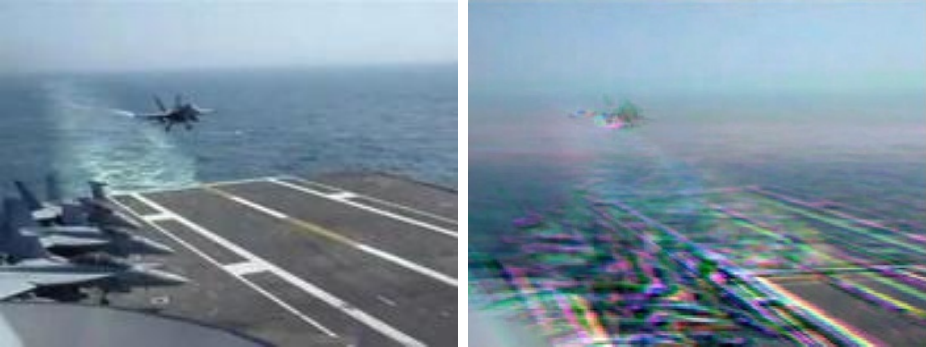
\includegraphics[height=2.1cm]{figures/related/fighter.png}
  \caption{Fighter dataset}
  \label{fig:aan_samples_fighter}
\end{subfigure}%
\begin{subfigure}{0.5\textwidth}
  \centering
  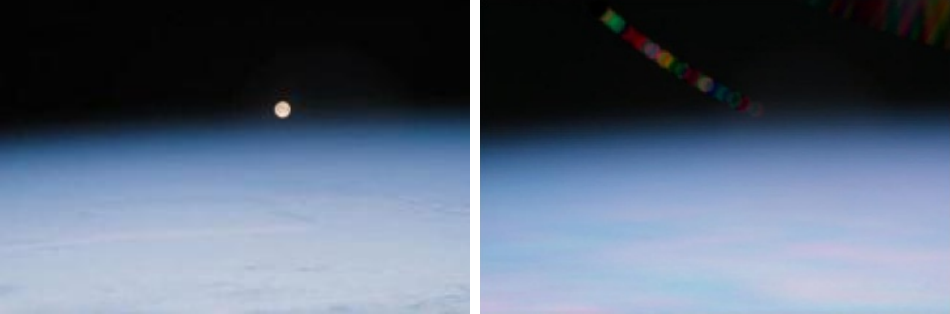
\includegraphics[height=2.1cm]{figures/related/nasa.png}
  \caption{NASA dataset}
  \label{fig:aan_samples_nasa}
\end{subfigure}
\caption[ANN Frame Prediction]{Single frame predictions using an ANN model with two hidden layers.\\
Left: ground truth target frame. Right: generated prediction. (From \parencite{ann})}
\label{fig:aan_samples}
\end{figure}

The loss during the training process was measured in terms of the MS-SSIM index in order to optimize the network to preserve the luminance, constrast and structure of the image. Since the data of the used Fighter and NASA datasets have a high image size, applyting the multi-scale version of SSIM was a reasonable choice.

When we take a look at the presented prediction results of Figure \ref{fig:aan_samples}, it can be seen that the network more or less averages over the input sequence. This effect is clearly visible in Figure \ref{fig:aan_samples_nasa}, were the movement of the moon from the top left towards the earth's horizon is predicted as a like composed of previous moon positions. As a result, this simple architecture does not sufficiently capture the temporal correlations of the input data.

\section{Recurrent Network Approaches}

In order to leverage the sequential structure and temporal correlations of video data, severals works performed frame prediction based on recurrent network models. These following models have inspired our overall model architecutre the most.

\subsection{LSTM Autoencoder Model}

A huge step forward has been taken when the recurrent encoder-decoder framework, earlier presented in Section \ref{sec:rnn_enc_dec}, has been applied in \parencite{unsup_learn_lstm} to perform unsupervised learning of video representations. The fact that the same operation must be applied at each time step to produce the next state was their key idea to use this framework in that context. 

All in all, a LSTM autoencoder model has been presented that was trained to reconstruct an entire input sequence of about ten image frames, similar to Figure \ref{fig:rnn-autoencoder}. This model has been slightly modified in a second step to predict the future sequence of frames. In a last step, both models have been combined to a model that exhibits a single encoder to learn the dynamics of the video, but two different encoders. Initialized by the identical learned representation, the one decoder tries to reconstruct the inputs backward in time, while the other decoder predicts the future frames forward in time. Consequently, the decoder has to come up with a represention that be handled by both decoders. In this way, they tried to compensate the shortcomings of each model, such as the potential tendency of reconstruction decoder to learn the trivial function, or to counteract that the future predictor considers the last frames of the input sequence only. This combined model delivered the best results and is shown in Figure \ref{fig:lstm_combo}.

\begin{figure}[htb]
	\centering
	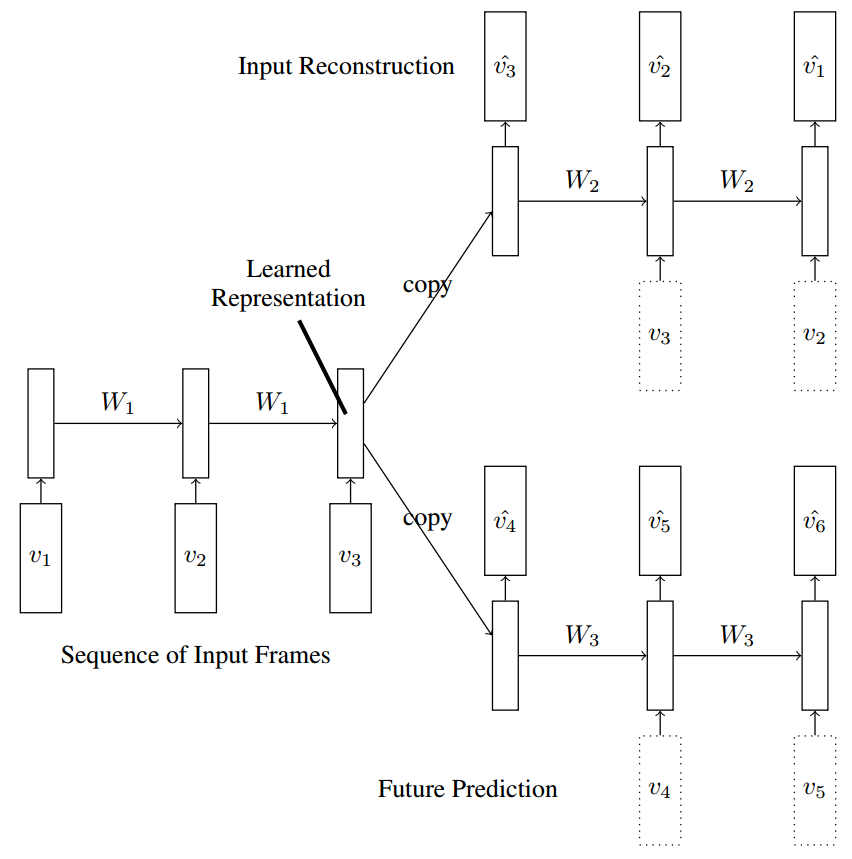
\includegraphics[width=0.5\linewidth]{figures/related/combo_shrinked.png} 
	\caption[Composite LSTM Autoencoder Model]{The composite LSTM autoencoder model. The top branch reconstructs the input sequence backwards in time, while the bottom branch performs frame predictions forward in time.} \label{fig:lstm_combo}
\end{figure}

Within their work, they also explored if the decoder should condition on the previously generated outout or not, as earlier discussed in Section \ref{sec:rnn_enc_dec}. The eventual choice has fallen on the conditioned variant, because it delivered slightly sharper frame predictions in the qualitative evaluation. Besides that, they also varied the number of recurrent layers with the clear result that a deeper LSTM yields best performance.

Another contribution of this work has been the introduction of a simple dataset that can be generated on-the-fly in order to explore the architecture of the model, as well as the effects of hyperparameter changes. It uses handwritten numbers that bounce around in a short sequence of images. Since this dataset has been used in several other subsequent works as well, it offers the ability to be used as a basic benchmark to compare the performance of various models. The dataset will be presented in detail in Section \ref{sec:ds_mm}. Sequences from these and another dataset have then been used as input to the LSTM encoder to train the model. It is to highlight, that they used the full image patch for this purpose. They mentioned to use convolutional percepts of the image sequence as inputs as well, but actually used this approach in the seconds part of their paper only, where they transfered the pre-trained encoder to improve the performance of supervised human action classification in videos.

The authors also pointed out that the choice of the loss function is fundamental with respect to quality of results. Nevertheless, they descided to rely on standard error functions and kept the use of more advanced objective functions for furhter research. To be more precise, they trained their network using binary cross-entropy when applied to MovingMNIST, and squared error for real world tests on UCF-101. Details about the latter dataset can be found in Section \ref{sec:ds_ucf}.

All in all, the strength of this model regarding future frame prediction is that it is able to infer a variable number of frames by taking the temporal correlations of the entire input sequence into account. But as a downside, the use of FC-LSTM cells with such high dimensional inputs implies a huge model complexity in the order of $10^8$ in case of a two-layer LSTM with \num{2048} hidden units each. Consequently, such a model takes a very long time to learn and does not consider spatial properties of each single input, due to the use of fully-connected state transitions.


\subsection{Convolutional LSTM Encoding-Forcasting Model}


\begin{figure}[htb]
	\centering
	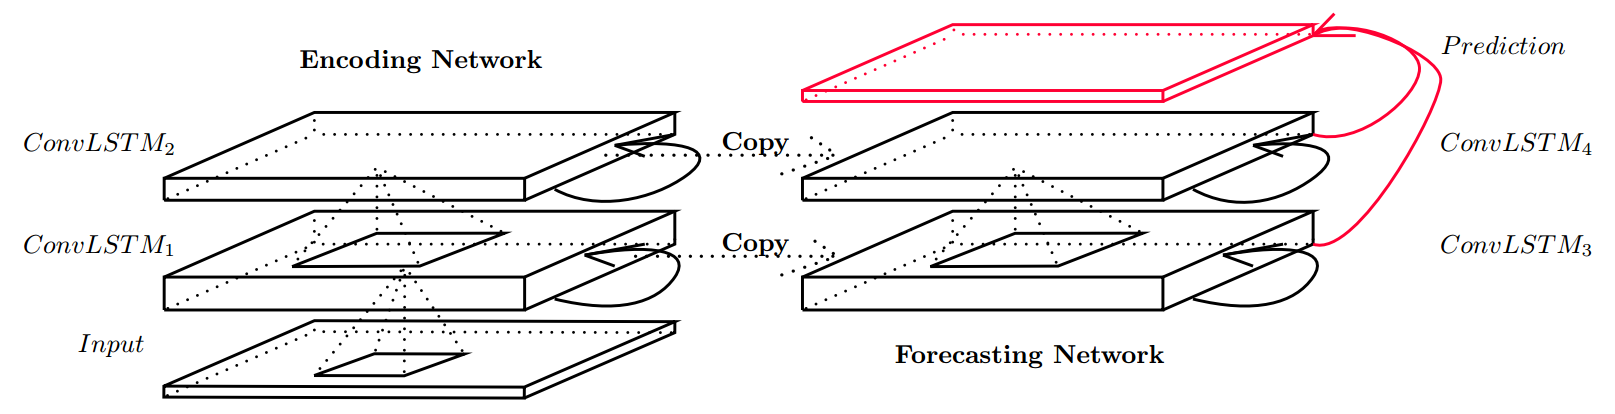
\includegraphics[width=0.8\linewidth]{figures/related/nowcasting_model.png} 
	\caption[Short]{Description.} \label{fig:convlstm_model}
\end{figure}

\subsection{Spatio-Temporal Video Autoencoder Model}

\begin{figure}[htb]
	\centering
	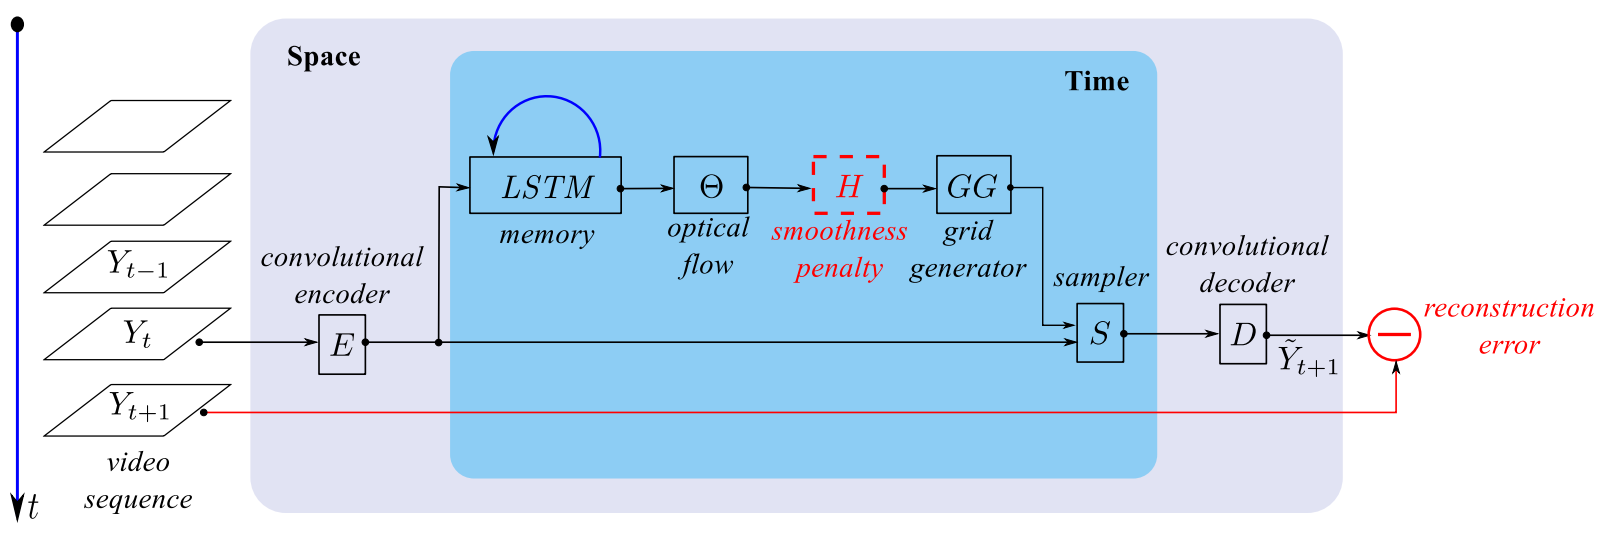
\includegraphics[width=0.8\linewidth]{figures/related/spat_temp_video.png} 
	\caption[Short]{Description.} \label{fig:spatiotemp_model}
\end{figure}


\begin{figure}[htb]
	\centering
	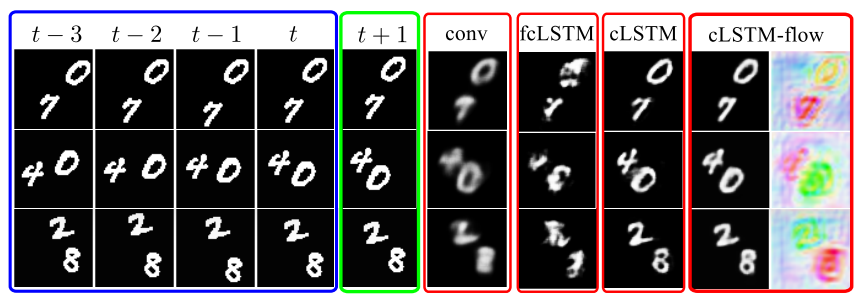
\includegraphics[width=1.0\linewidth]{figures/related/spat_temp_results.png} 
	\caption[Short]{Description.} \label{fig:spatiotemp_results}
\end{figure}


\section{Adversarial Network Approach}


\begin{figure}[htb]
	\centering
	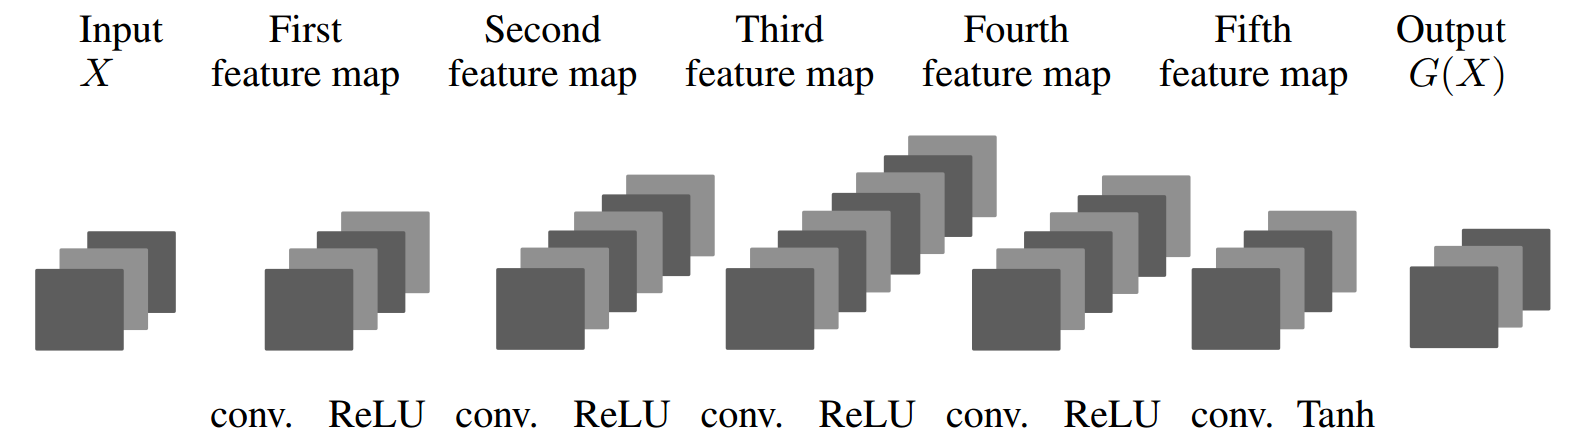
\includegraphics[width=0.8\linewidth]{figures/related/deep_multiscale_generator.png} 
	\caption[Short]{Description.} \label{fig:gan_generator}
\end{figure}


\begin{figure}[htb]
	\centering
	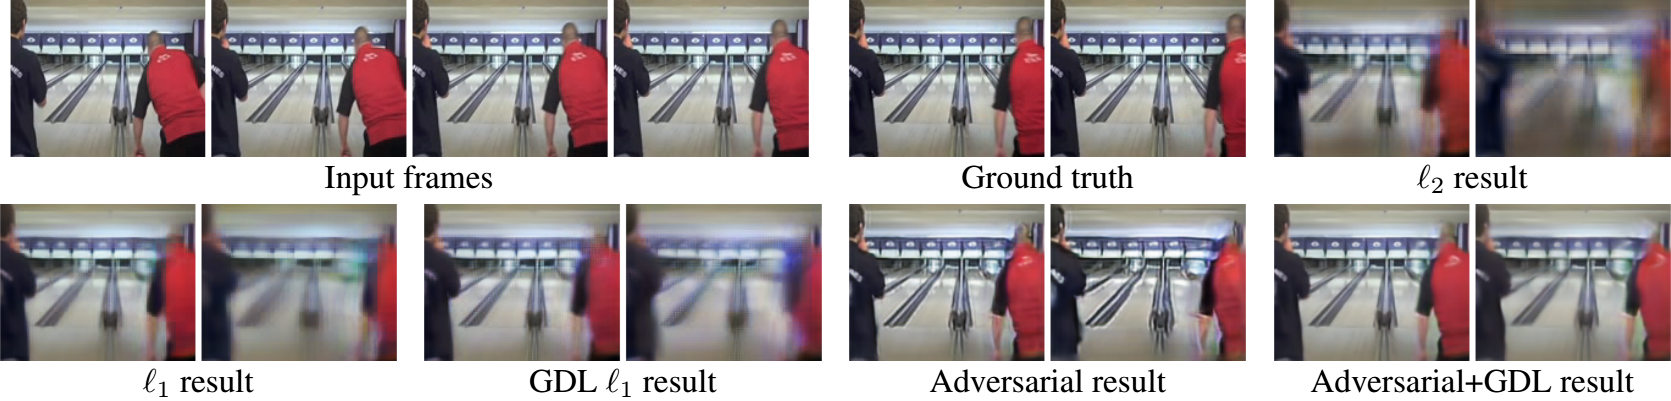
\includegraphics[width=1.0\linewidth]{figures/related/deep_multiscale_samples.png} 
	\caption[Short]{Description.} \label{fig:gan_samples}
\end{figure}





%In \textbf{Chapter \ref{chapter:relatedwork}}, we take a closer look at existing approaches that are suitable for spatio-temporal learning and frame prediction. We briefly discuss their strength and weaknesses, as well as how they have influenced the design decisions regarding the architecture of our final neural network model. Additionally, these presented models build the baselines in our evaluation.
\skippage
% !TeX root = ../main.tex

\chapter{A Fully-Convolutional LSTM Encoder-Predictor Model} \label{chapter:implementation}

This chapter presents the final model that is used in this thesis for future frame prediction. It combines the insights and strengths of previous works that have been analyzed in the preceding chapter. Each component of it is investigated in detail and then assembled to end up with the overall network architecture. But beforehand, two cruicial techniques are presented which improve the learning of spatio-temporal features and the recurrent training performance.

\section{Techniques}

In this section, two important methods are presented that enable recurrent network based models to reach better performance in a shorter time of training. The next section then uses these techniques as building blocks while describing the network architecture.

\subsection{Convolutional LSTM} \label{sec:conv_lstm}

As discussed in earlier chapters, the standard LSTM cell has the drawback of lacking spatial correlations in the input-to-hidden and hidden-to-hidden transitions, because it operates over sequences of vectors with only one dimension. The LSTM activations are computed based on linear transformations using fully-connected layers and subsequent non-linearities. The authors of \parencite{conv_lstm_nowcasting} propose a variant of the LSTM cell with the core idea to handle all inputs, hidden states, cell or gate outputs as 3D tensors to preserve the spatial data properties. This is realized by exchanging the internal matrix products by convolution operations. The resulting recurrent cell type is called \textit{convolutional LSTM} (ConvLSTM).

In contrast to the realization in \parencite{spat_temp_video_autoenc}, peephole connections are included in our implementation of ConvLSTM. These allow the gated units to have a direct access to the previous memory cell state. In addition, we enable it to use optional batch normalization layers in both input-to-hidden and hidden-to-hidden transitions to allow faster learning and to take advantage of its other benefits which have been described in section \ref{sec:batch_norm}. The same modifications have been proposed for the standard LSTM cells in \parencite{rnn-batchnorm}. All this together can be formulated as:

%TODO maybe correct this formula, since we used conv2d instad of hadamard for peepholes as well.
\begin{equation} \label{eq:convlstm}
\begin{aligned}
\Spvek{\tilde{\textbf{f}}^{(\tau)}; \tilde{\textbf{i}}^{(\tau)}; \tilde{\textbf{o}}^{(\tau)}} &= \texttt{BN}(\textbf{W}_{h} \ast \textbf{h}^{(\tau-1)}; \gamma_h, \beta_h) + \texttt{BN}(\textbf{W}_{x} \ast \textbf{x}^{(\tau)}; \gamma_x, \beta_x) + \textbf{W}_{peep} \odot \textbf{C}^{(\tau-1)} + \textbf{b} \\
\hat{\textbf{c}}^{(\tau)} &= tanh(\texttt{BN}(\textbf{W}_{hc} \ast \textbf{h}^{(\tau-1)}; \gamma_h, \beta_h) + \texttt{BN}(\textbf{W}_{xc} \ast \textbf{x}^{(\tau)}; \gamma_x, \beta_x) + \textbf{b}_c) \\
\textbf{C}^{(\tau)} &= \sigma(\tilde{\textbf{f}}^{(\tau)}) \odot \textbf{C}^{(\tau-1)} + \sigma(\tilde{\textbf{i}}^{(\tau)}) \odot \hat{\textbf{c}}^{(\tau)} \\
\textbf{h}^{(\tau)} &= \sigma(\tilde{\textbf{o}}^{(\tau)}) \odot tanh(\texttt{BN}(\textbf{C}^{(\tau)}; \gamma_c, \beta_c))
\end{aligned}
\end{equation}

where $ \textbf{W}_h \in \mathbb{R}^{d_h \times 3d_h} $ and $ \textbf{W}_{hc} \in \mathbb{R}^{d_h \times d_h} $ are the shared weights for the hidden-to-hidden transitions at time step $ \tau $, $ \textbf{W}_x \in \mathbb{R}^{d_x \times 3d_h} $ and $ \textbf{W}_{xc} \in \mathbb{R}^{d_x \times d_h} $ the shared weights for the input-to-hidden connections, as well as $ \textbf{W}_{peep} \in \mathbb{R}^{d_x \times 3d_h} $ the shared weights for the peephole connections. Next, $ \textbf{b} \in \mathbb{R}^{3d_h} $ and $ \textbf{b}_c \in \mathbb{R}^{d_h} $ are the biases, $ \textbf{C}^{(0)}, \textbf{h}^{(0)} \in \mathbb{R}^{4d_h} $ the initial states of the memory cell and the hidden state, respectively. Furthermore, $\ast$ denotes the convolution operation and $ \texttt{BN}(\textbf{x}; \gamma, \beta) $ a batch normalization layer with its learned shift $\gamma$ and scale $\beta$. As in \parencite{rnn-batchnorm}, $\beta_h$ and $\beta_x$ are set to zero by default to avoid the unnecessary redundancy with the existing bias terms $\textbf{b}$ and $\textbf{b}_c$. The structure of such a cell is visualized in Figure \ref{fig:convlstm-cell}.

\begin{figure}[htpb]
	\centering
	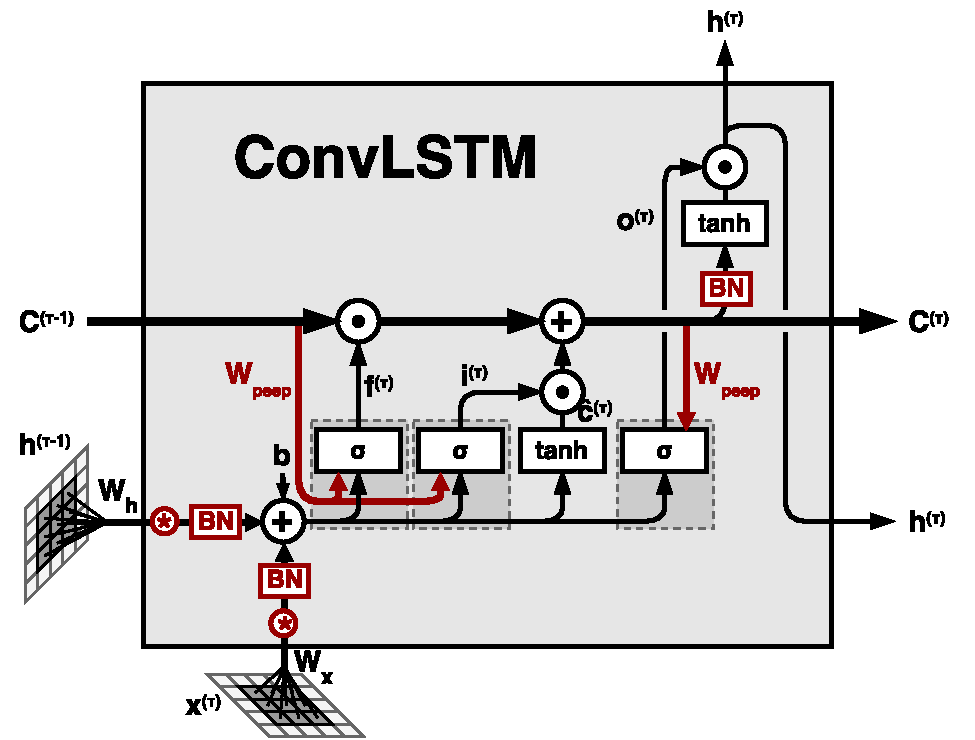
\includegraphics[width=0.65\linewidth]{figures/convlstm.pdf} 
	\caption[ConvLSTM Cell]{The simplified structure of the batch-normalized ConvLSTM cell including peephole connections. The inputs and previous hidden states are convolved to produce 3D tensors that flow through each cell. Changes to standard FC-LSTM are highlighted in red.} \label{fig:convlstm-cell}
\end{figure}


\subsection{Scheduled Sampling} \label{sec:sched_sample}

When the first recurrent network based models have been tested in the course of this thesis, a discrepancy between training and inference has been discovered. At training time, each cell is usually fed with the ground truth $\textbf{x}^{(\tau-1)}$ of the previous time step in order to generate the current prediction $\hat{\textbf{x}}^{(\tau)}$. In contrast, the generated frame $ \hat{\textbf{x}}^{(\tau-1)}$ of the previous cell is used instead as cell input during inference, because no ground truth is available in that case. Thus, mistakes made earlier in the sequence flow through all following cells and can quickly amplify since the network has never dealt with such errors at training time. In context of future frame generation, this effect has been identified when the prediction quality has dropped tremendously after the first generated frame. The fact that predicted frames usually look slightly blurry is the clear reason for this, because a network that was fed purely with ground truth input images has never seen such pictures with smooth edges.

As a first step, the recurrent cell input during the training process has therefore been adapted to behave in the same way as in inference mode. Therefore, a recurrent cell that is trained to generate a future frame has to condition on the previously generated frame instead of the ground truth\footnote{Always conditioning on the generated outputs while training is called \textit{always sampling} (AS) according to \parencite{sched_sample}.}. This strategy can be seen as an automatic form of data augmentation or a natural regularizer and helps the network to learn a robustness against imperfect inputs. However, this comes with the downside that the RNN model converges much slower during the training, because it has to predict the correct output given poor or even wrong input data.

To combine the best of both worlds, we have experimented with a training strategy where each recurrent cell started to condition on the ground truth frame and have slowly changed to the inference mode conditioning using a probability variable $p$ with linear or exponential decay. In this process, a random number $r \in [0, 1]$ is generated at each training step and the RNN cells condition on the generated frame when $r \geq p$. First experiments have shown positive results, because a better performance could be reached compared to both other strategies mentioned earlier. 

Shortly afterwards, we came across \parencite{sched_sample} where the authors propose a similar but even more radical strategy and demonstrate insightful evaluation results. Their so-called \textit{scheduled sampling} (SS) training strategy for recurrent networks is based on the same core idea, but instead of generating only a single random number $r$ for the whole input sequence, they propose to do this for every single time step $\tau$. In addition, they suggest to use an inverse sigmoid decay function in order to provide a smooth transition from training mode to inference mode:

\begin{equation} \label{eq:inverse-sigmoid}
\sigma_{inv}(i; \alpha) = \frac{\alpha}{\alpha + exp(i / \alpha)} ,
\end{equation}

where $i$ identifies the current training step and $\alpha \geq 1$ controls the expected speed of convergence. This function and a diagram of the scheduled sampling approach is depicted in Figure \ref{fig:sched-sample}.

\begin{figure}[htpb]
\centering
\begin{subfigure}{0.5\textwidth}
  \centering
  \hspace*{-0.6cm}
  {
  \begin{tikzpicture}[scale=0.75]
    \begin{axis}[
        ymin=-0.1,
        ymax=1.1,
        xmin=0,
        xmax=1000,
        legend style={legend pos=north east},
        grid,
        thick,
        ylabel=GT sampling probability \textit{p},
        xlabel=step \textit{i},
      ]
      \addplot [mark=none,draw=LightGoldenrod,smooth,ultra thick,domain=0:1000] {75/(75+exp(\x / 75))};
      \addlegendentry{inverse sigmoid ($\alpha = 75$)};
    \end{axis}
  \end{tikzpicture}
  }
  \caption{}
  \label{fig:sched-sample-inv-sig}
\end{subfigure}%
\begin{subfigure}{0.5\textwidth}
  \centering
  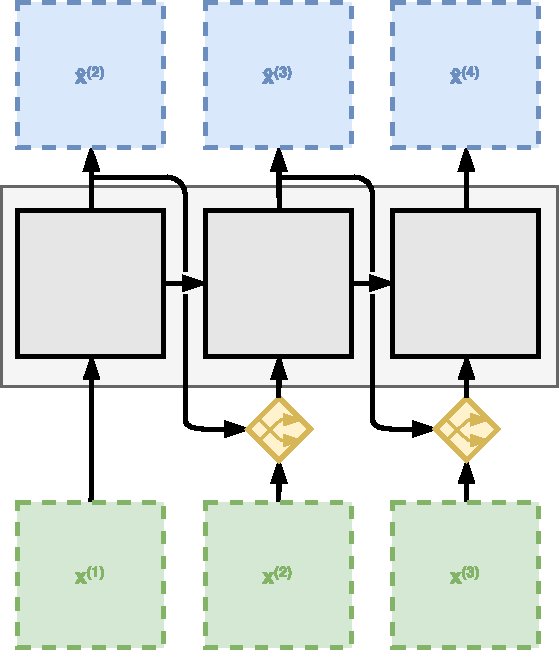
\includegraphics[width=.7\linewidth]{figures/sched_sample.pdf}
  \caption{}
  \label{fig:sched-sample-process}
\end{subfigure}
\caption[Scheduled Sampling]{Illustration of scheduled sampling, where (a) shows the inverse sigmoid decay function and (b) the structure of a RNN that uses this approach. The yellow blocks symbolize the scheduled sampling components, which decide whether a cell conditions on the ground truth or the previous output by flipping an unbiased coin.} \label{fig:sched-sample}
\end{figure}




\section{Network Architecture}

The final model architecture is based on the RNN encoder-decoder framework introduced in Section \ref{sec:rnn_enc_dec} and both previously presented advancements to improve the learning of spatio-temporal features in video data. This architecture has been chosen because it explicitly models the temporal correlations and is flexible regarding the input and output sequence. Further, previous works demonstrated in Chapter \ref{chapter:relatedwork} have shown promising results using this recurrent framework. The architecture that is presented in this section describes the default version of the network that is used for frame prediction of generated image sequences of animated, handwritten numbers. The following evaluation in Chapter \ref{chapter:evaluation} assesses this model with different settings, such as variations in the network's depth.

\subsection{Components} \label{sec:impl-components}

Before the entire network model is demonstrated, we would like to go through its main components in detail first. These components for encoding or decoding are ordered according to the flow of data while propagating forward through the network. Afterwards, the loss layer is presented which combines standard error functions with perceptual motivated bias terms.

\subsubsection{Spatial Encoder}

Instead of feeding the recurrent encoder directly with raw image data like in \parencite{unsup_learn_lstm} or \parencite{conv_lstm_nowcasting}, each frame flows through a multilayer CNN first. Therefore, it is projected to an image percept in feature space of lower size, but higher depth. This single convolutional network is shared across the entire time domain of the spatio-temporal encoder component described next. The motivation to use this spatial encoder is based on \parencite{spat_temp_video_autoenc} which suggests that a deeper encoding of the input image can yield better results. Furthermore, decreasing the height and width of the image has a positive impact on the overall runtime and memory efficiency. Although the number of feature maps and hence the dimensionality of the convolved frame percepts is higher compared to the original image, it does not harm these two advantages with respect to the total efficiency of the model. This is due the fact that the ConvLSTM cells and their convolutional state-to-state transitions within the following recurrent encoder increase the feature space representation's depth either way. The spatial encoder component is illustrated in Figure \ref{fig:comp-spatial_encoder}.






\begin{figure}[htb]
	\centering
	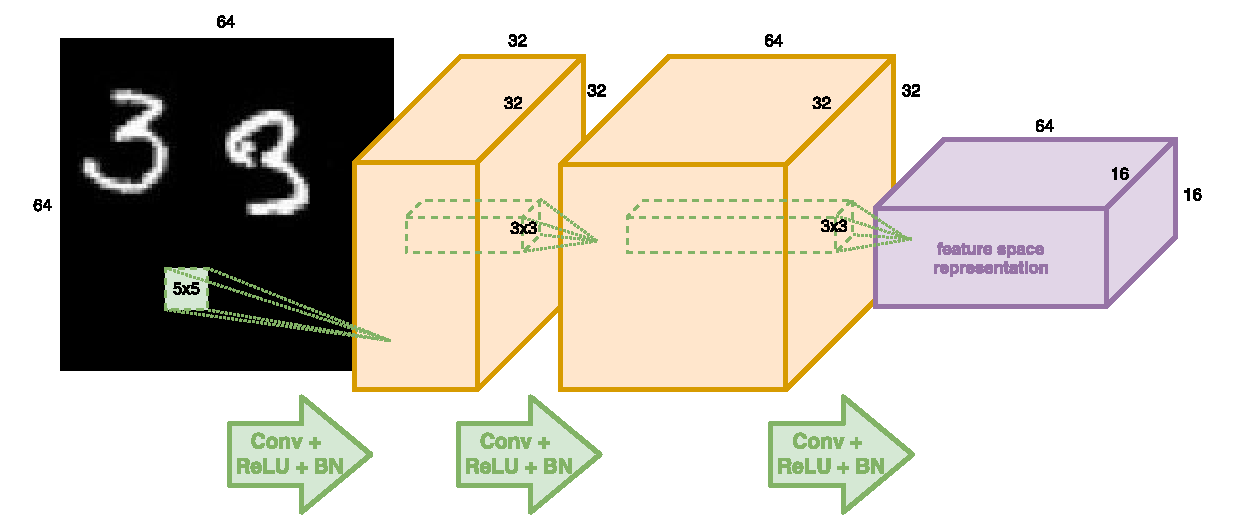
\includegraphics[width=0.9\linewidth]{figures/comp_spatial_encoder.pdf} 
	\caption[Spatial Encoder Component]{Spatial encoding network that maps each input image to its feature space representation (purple) using convolutional layers with ReLU activations and subsequent batch normalizations (green). Intermediate tensors (yellow) are denoted with their height, width and depth.} \label{fig:comp-spatial_encoder}
\end{figure}

No max pooling layers are used because rotation tolerance would be counter-productive in context of frame prediction. This kind of downsampling could remove important details that might be required to successfully reconstruct the image. Instead, each frame is downsampled by using a stride of $ s=2 $ in specific convolutional layers with the motivation that the network itself should learn how to perform such a downsampling operation. Additionally, each convolutional layer is activated using ReLUs and followed by a batch normalization layer to compensate the internal covariate shift of such a deep network model. The resulting frame percepts exhibit a shape of $16\times16\times64$.

\subsubsection{Spatio-Temporal Encoder}



After each percept tensor has been produced by the spatial encoder CNN, it then flows unchanged into a recurrent network to preserve sequential correlations and to learn temporal dynamics. To be more precise, ConvLSTM cells are used to retain the spatial structure of the three-dimensional input data. The cell state $C^{(0)}$ and hidden state $h^{(0)}$ of the spatio-temporal encoder network are initialized with zero by default. Moreover, all convolutional layers within the ConvLSTM cells adapt their number of produced features maps according to the input's depth in order to keep all shape sizes constant. After the whole input sequence of about ten frames has been processed, the resulting cell and hidden states of the last unit then encode the learned motion of the sequence. This representation is then transferred to the following prediction component. It should be noted that the hidden outputs of the encoder's ConvLSTM cells are discarted and not used in the subsequent decoding network. The spatio-temporal encoder component is shown in Figure \ref{fig:comp-spatiotemp_encoder}.

\begin{figure}[htb]
	\centering
	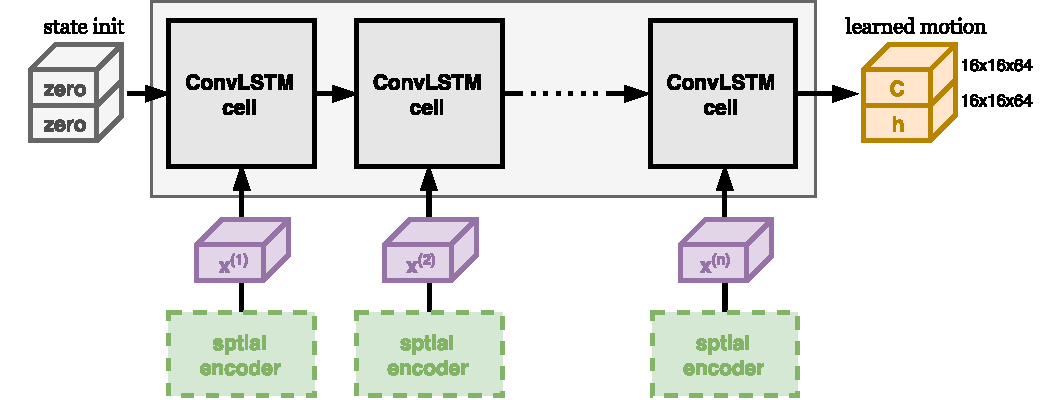
\includegraphics[width=0.9\linewidth]{figures/comp_spatiotemp_encoder.pdf} 
	\caption[Spatio-Temporal Encoding Component]{Spatio-temporal encoder network that encodes a motion representation (orange) based on a frame sequence in feature space (purple). The feature space representations are mapped from each single frame in image space and are produced by the previously described spatial encoder (green).} \label{fig:comp-spatiotemp_encoder}
\end{figure}

\subsubsection{Spatio-Temporal Predictor}

Initialized by the last cell and hidden state of the previous ConvLSTM encoder, the recurrent predictor component takes over to map each frame in feature space at time step $\tau$ to its future representation at time step $\tau + 1$. The spatio-temporal decoder takes advantage of the ConvLSTM cells once more, but it handles the inputs and outputs of each cell in a different way.

\begin{figure}[htb]
	\centering
	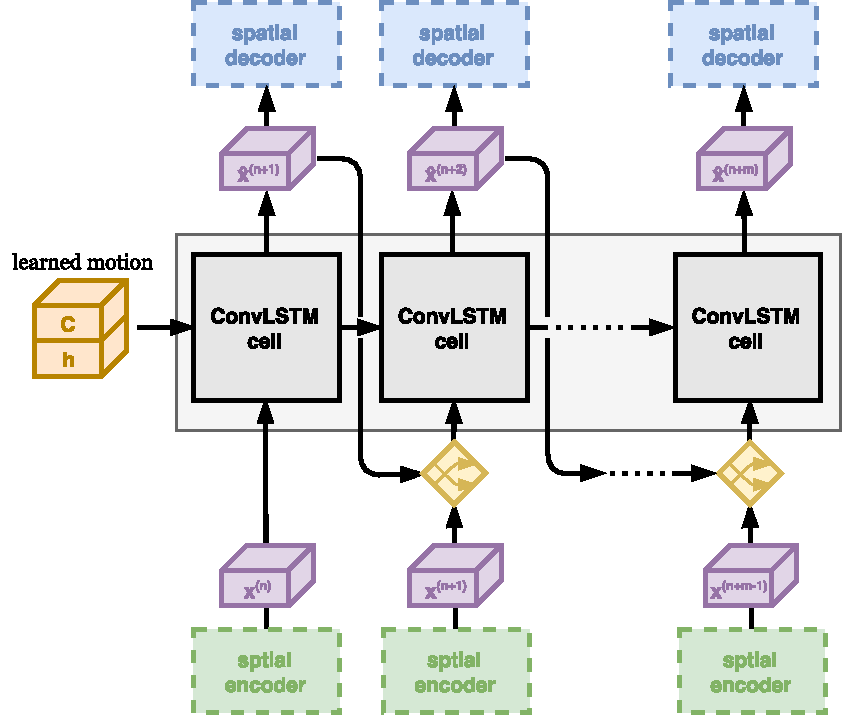
\includegraphics[width=0.8\linewidth]{figures/comp_spatiotemp_decoder.pdf} 
	\caption[Spatio-Temporal Predictor Component]{Spatio-temporal decoding network that maps a frame in future space to its future representation. The ConvLSTM is initialized with the learned motion representation (orange) produced by the recurrent encoder. Each ConvLSTM cell receives either the ground truth representation or the output of the previous cell as its input while training. This decision is made by scheduled sampling components (yellow) at each time step.} \label{fig:comp-spatiotemp_predictor}
\end{figure}

As depicted in Figure \ref{fig:comp-spatiotemp_predictor}, the prediction component utilizes the scheduled sampling technique, earlier presented in Section \ref{sec:sched_sample}, to improve the training performance. By default, the network begins to condition on ground truth frame representations in feature space that have been produced by the spatial encoder component. By decaying the probability of conditioning on the ground truth using an inverse sigmoid function with $\alpha = 1000$, the predictor RNN slowly starts to condition on previously generated frames like in inference mode. With this setting, it takes about \num{10000} training steps until this component predicts future frame representations entirely based on generated outputs. After the entire output sequence has been generated, each single tensor still exhibits a shape of size $16\times16\times64$ and altogether represent the video's future in feature space.

\subsubsection{Spatial Decoder}

To map each frame representation back to the image space, a second CNN is modelled that performs the same transformation steps of the spatial encoder but in reverse order. It therefore uses transposed convolutional layers with rectifier units and batch normalization layers in-between. However, the activation function of the output layer is either a sigmoid or a hyperbolic tangent function to ensure that the generated frames exhibit a valid scale of values. The described spatial decoder is illustrated in Figure \ref{fig:comp-spatial_decoder}.

\begin{figure}[htb]
	\centering
	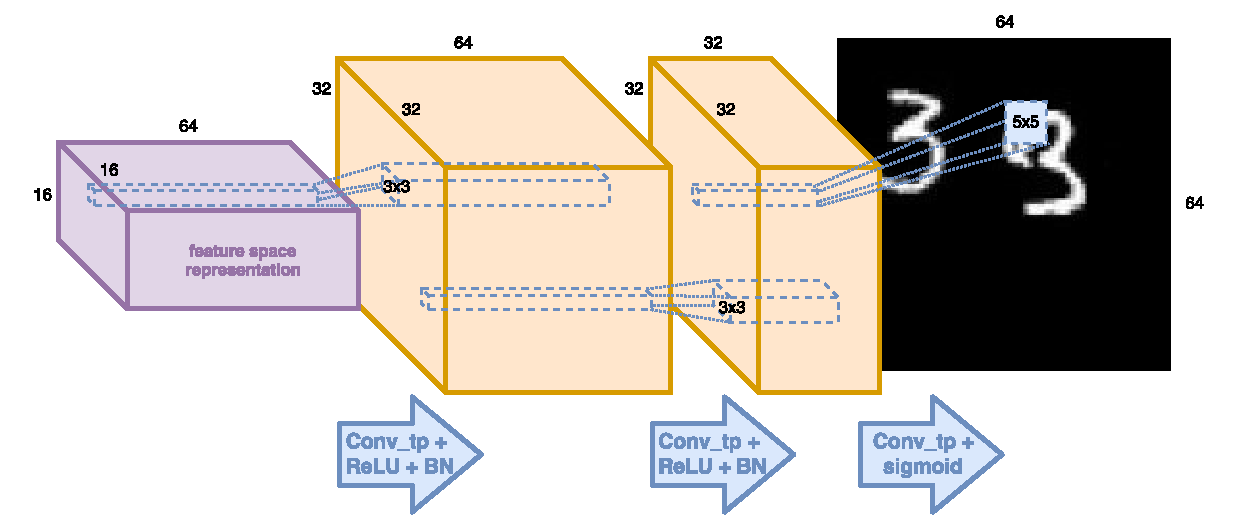
\includegraphics[width=0.9\linewidth]{figures/comp_spatial_decoder.pdf} 
	\caption[Spatial Decoder Component]{Spatial decoding network, which learns to reverse the mapping of the spatial decoder using transposed convolutional layers (blue), to map a feature space representation back to original image space.} \label{fig:comp-spatial_decoder}
\end{figure}


\subsubsection{Loss Layer}

The last component which has to be mentioned is the loss layer used while training the model. Since previous works have shown the problems of using standard loss functions like $\ell_2$ in image processing tasks, as earlier described in Section \ref{sec:perc-loss}, the main objective $\mathcal{L}_{\textrm{main}}$ used in this work is extended by two perceptual motivated bias terms that respect the human notion of visual similarity. The main loss function itself is a placeholder for any commonly used loss function. Depending on the data characteristics, we therefore use $\mathcal{L}_{\textrm{bce}}$, $\mathcal{L}_{\textrm{mse}}$ or $\mathcal{L}_{\textrm{mae}}$ in our context. To counteract the lack of sharpness in predicted frames, a GDL objective function is used as a first extension in order to quantify the sharpness of the image. As a second extension, the SSIM-based loss function is used to assess the image's luminance, contrast and structure. The SSIM-kernel size is chosen to be $k=5$, reasoned by the fact that small image patches are used during the training process only, as well as to improve computational efficiency. The same reasons have also led to the decision to not use the MS-SSIM index. Moreover, RGB image patches are temporarily converted to grayscale which is required to calculate the structural similarity index. Combining these three loss terms together with different weights results in the \textit{triplet loss function} that is used within our experiments:

\begin{equation} \label{eq:triplet}
\mathcal{L}_{\textrm{triplet}}(\textbf{X}, \hat{\textbf{X}}) = \lambda_{\textrm{main}} \mathcal{L}_{\textrm{main}}(\textbf{X}, \hat{\textbf{X}}) + \lambda_{\textrm{gdl}} \mathcal{L}_{\textrm{gdl}}(\textbf{X}, \hat{\textbf{X}}) + \lambda_{\textrm{ssim}} \mathcal{L}_{\textrm{ssim}}(\textbf{X}, \hat{\textbf{X}}) ,
\end{equation}

where $ \textbf{X} $ denotes the ground truth target sequence and $ \hat{\textbf{X}} $ the network's predicted future sequence. The weight and bias parameters of each loss function are neglected for the benefit of simplicity. The coefficients $\lambda_{\textrm{main}}$, $\lambda_{\textrm{gdl}}$ and $\lambda_{\textrm{ssim}}$ control the relative importance of each component in the triplet loss function. A simple default setting is to weight them equally by setting $\lambda_{\textrm{main}} = \lambda_{\textrm{gdl}} = \lambda_{\textrm{ssim}} = 1$.

Additionally, experiments similar to \parencite{gen_img_perc_sim} have been performed where a further loss has been injected to quantify the similarity of feature space representations. Unfortunately, we could not improve our results with such an additional term, because it is not trivial to find an appropriate coefficient $\lambda_{\textrm{feat}}$ to weight this feature space loss relative to other image space losses. On the one hand, it has no visible effect when the coefficient is chosen too low. On the other hand, the accuracy of the predictions decreases tremendously when the coefficient is chosen too high. Due to the difficulties in finding a good balance, as well in the interest of time, such a feature space loss is not used in the final model.


\subsection{Model}

For a better overview regarding the resulting model complexity, Table \ref{tab:model_params} lists the number of trainable parameters for each network component described previously.

\begin{table}[htpb]
  \small
  \centering
  \begin{tabular}{l r}
    \toprule
      \textbf{Component} & \textbf{Trainable parameters} \\
    \midrule
      Spatial encoder \scriptsize{(CNN)} & \num{56416} \\
      Spatio-temporal encoder \scriptsize{(ConvLSTM)} & \num{864512} \\
      Spatio-temporal decoder \scriptsize{(ConvLSTM)} & \num{864512} \\
      Spatial decoder \scriptsize{(CNN)} & \num{56353} \\
    \midrule
    \midrule
      \textbf{Total} & \textbf{\num{1841793}} \\
    \bottomrule
  \end{tabular}
  \caption[Model Parameters]{Overview of the network parameters per component in the described vanilla setting using 1-layer ConvLSTMs.}\label{tab:model_params}
\end{table}

To see everything at a glance, each component is put together in Figure \ref{fig:total_model} to demonstrate the entire model. It has to be noted that not every depicted building block or connection is used when a future sequence is predicted within an inference step. For example, only half as many frames have to be processes by the spatial encoder, because the feature representations of the ground truth target sequence are obviously not available when an actual future prediction is performed. The same is also true for the scheduled sampling components and the loss layer that are only required to train the model. Additionally, the data tensors of each single frame is processed by a separate CNN. Therefore, the trainable parameters in each convolutional layer of the spatial encoder and decoder has to be shared across the whole input sequence. 

Since the overall architecture follows the concept of an encoder-decoder network, it should be argued why this model is likely to learn useful features. According to the argumentation in \parencite[p. 3f.]{unsup_learn_lstm}, it is unlikely to learn the trivial function for the following two reasons. First, an entire sequence of variable size as well as the temporal dynamics have to be encoded and decoded using a fixed-sized representation. In order to accurately predict future frames multiple time steps ahead, the decoder network really has to come up with a learned representation that can distinguish several foreground objects from static background, as well as understand the motion of object and the environmental constraints within a given video scene. Second, the learned motion pattern has to generalize well so that it can be applied to any time step of the sequence. Performing a simple copy of the last state might be almost sufficient when a single frame is predicted only, but not when it has to look further into the future.

\begin{figure}[p]
	\centering
	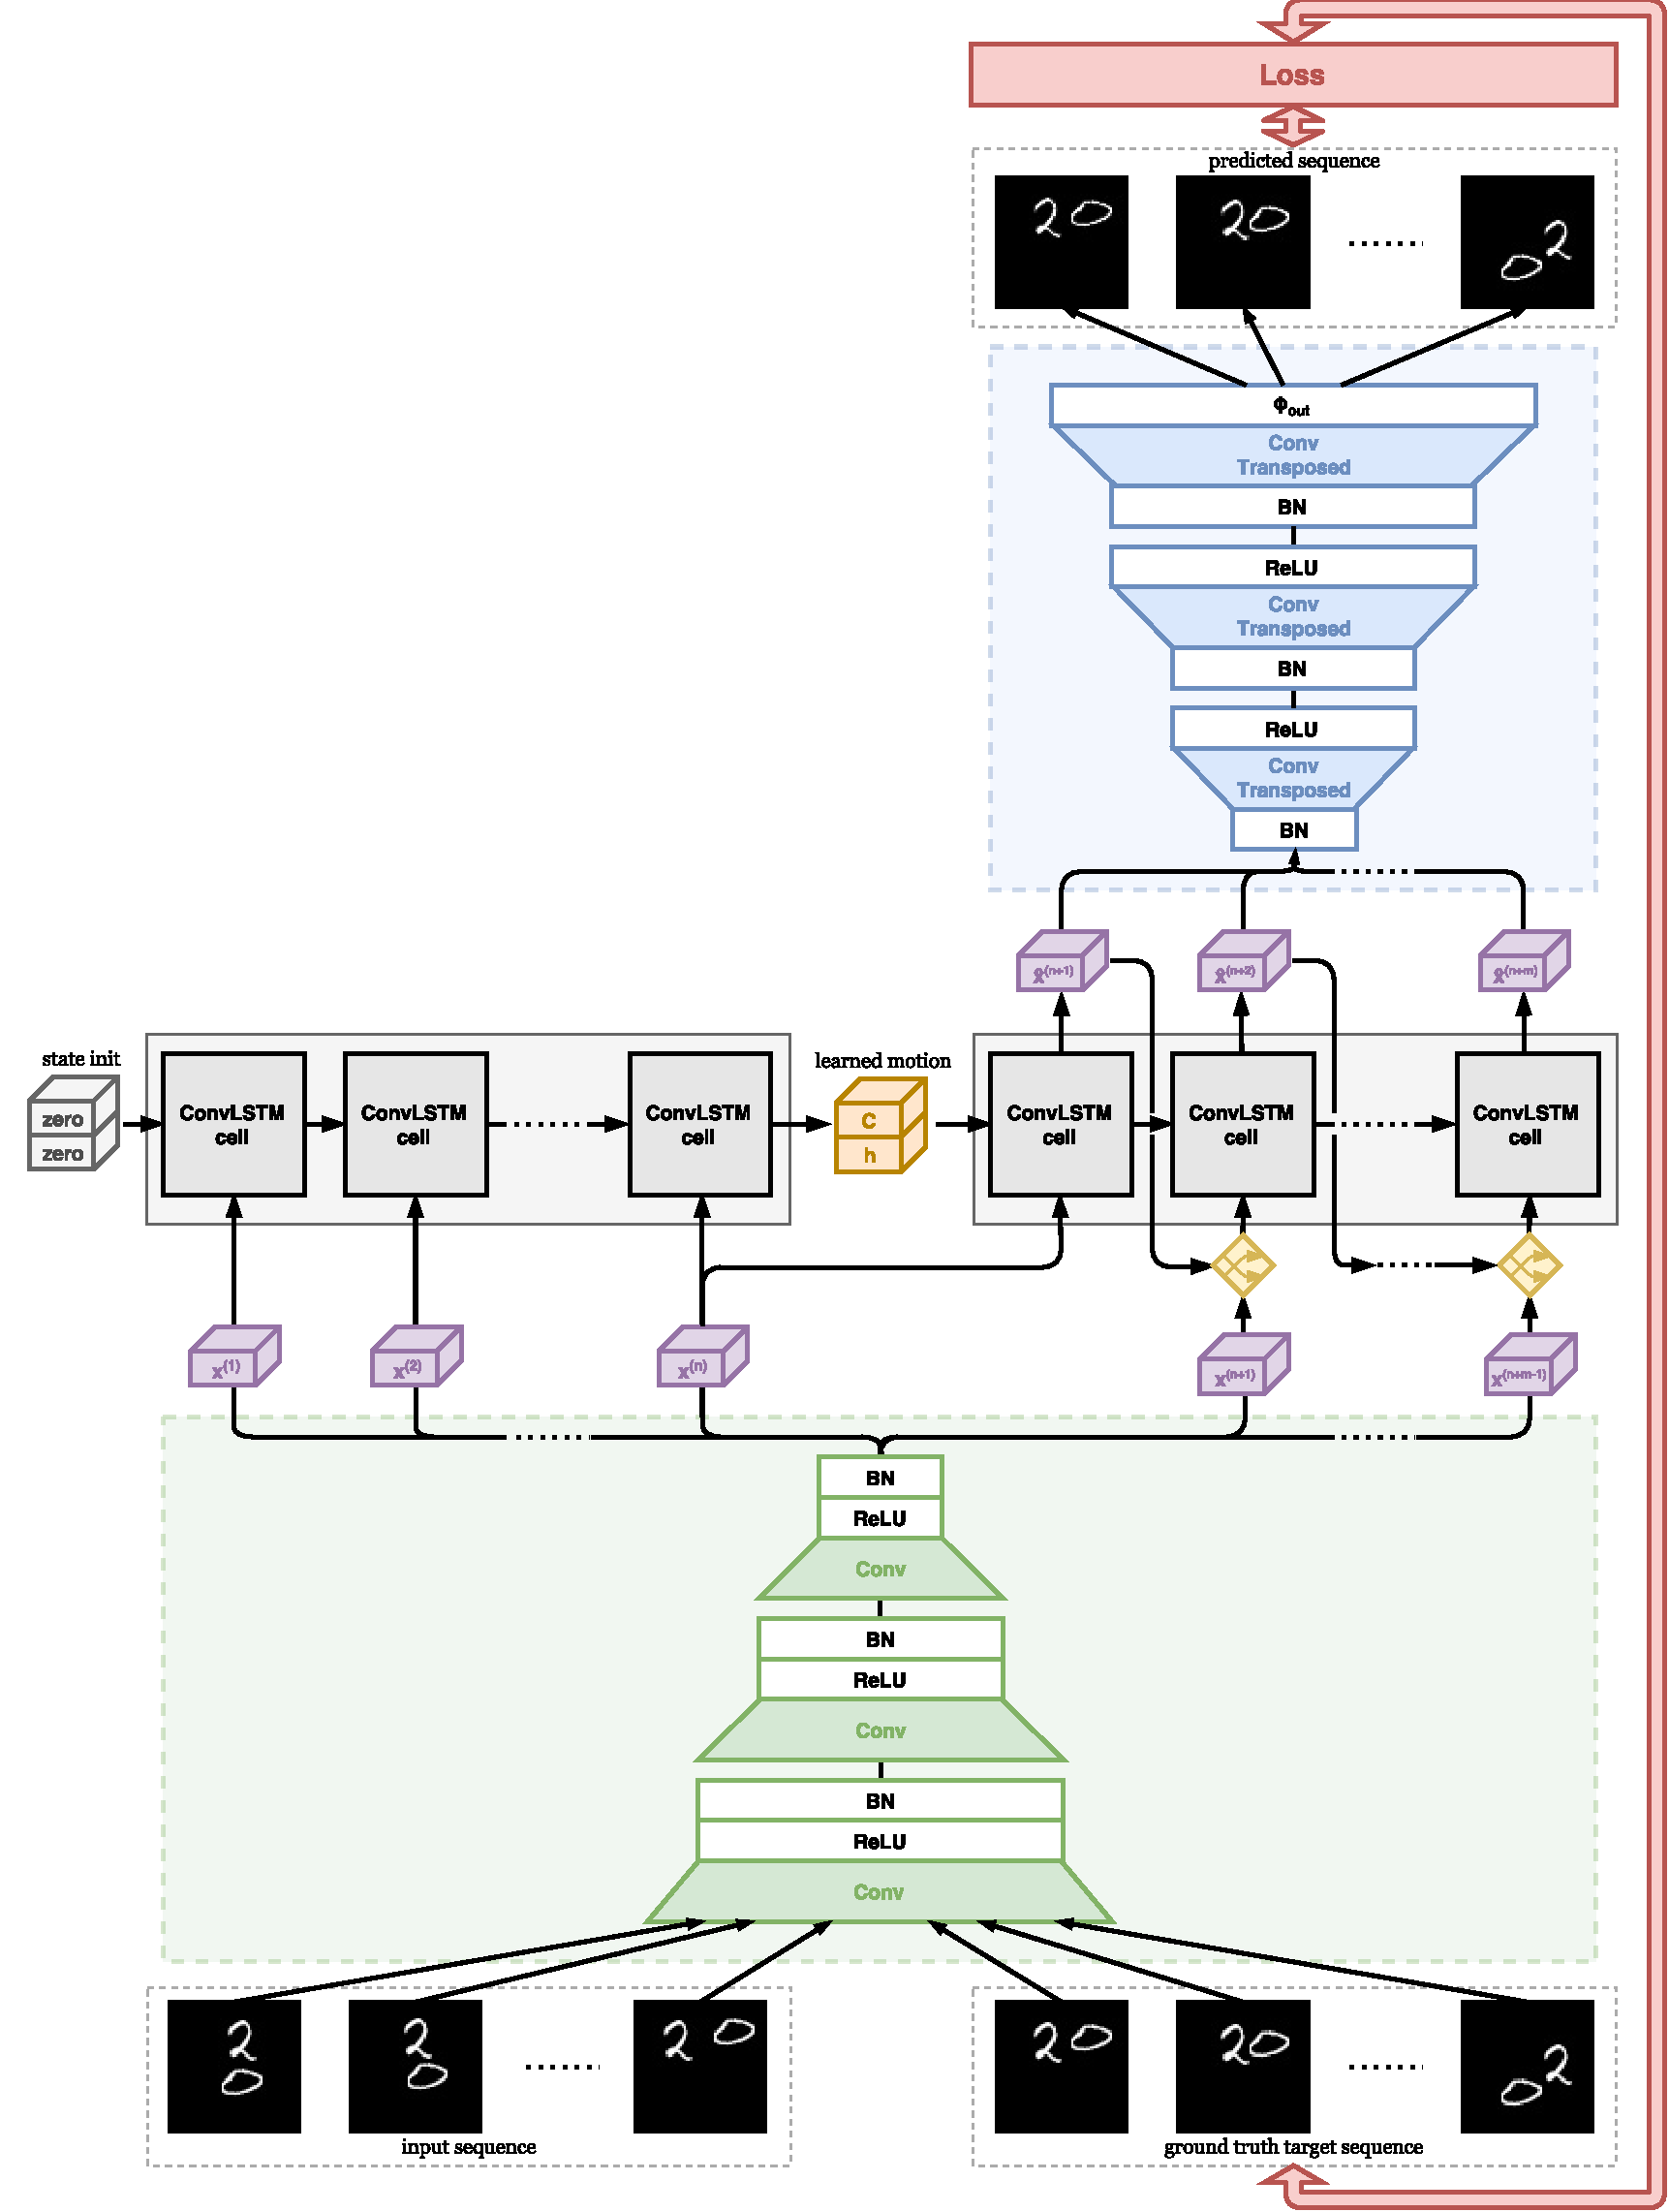
\includegraphics[width=0.96\linewidth]{figures/total_model.pdf}
	\caption[ConvLSTM Encoder-Predictor Model]{The ConvLSTM Encoder-Predictor Model. Weights of the convolutional encoder (green) and decoder (blue) are shared layer-wise across the whole sequence. Spatial encodings of the ground truth frames, scheduled sampling components (yellow) and the loss layer (red) are only used while training.} \label{fig:total_model}
\end{figure}

\skippage
% !TeX root = ../main.tex

% why not Sport M1 dataset
% why we used crops
% why we used which input-output length
% why we used movement-detection (any describe how)
% how we define an epoch for each
% dataset details (overview as a table?)
% why we used these datasets

% UCF / PAC: show patches AND full-images seq. examples :)



\chapter{Datasets} \label{chapter:datasets}

This chapter presents all datasets that are going to be used in the following evaluation. We have chosen three different video datasets that have been used in related works in order to be able to compare the results and analyze the strength and weaknesses of the different network models. The selected datasets will be introduced one after another ordered by their content's complexitiy with respect to the possible variations in colors, motion and pysical environment. Additionally, random samples from each dataset will be shown to get a better idea of how the data that is fed to the network looks like.


\section{Moving MNIST}


We first train our model on a synthetic dataset of black and white images with flying handwritten digits. The \textit{Moving MNIST} was firstly introduced in \parencite{unsup_learn_lstm} and applied in context of video frame prediction. Since then, it was used several times in different follow-up works, such as \parencite{spat_temp_video_autoenc} or \parencite{conv_lstm_nowcasting}. 

\subsection{Data Generation and Characteristics}

In the proposed setting, each sequence consists of $20$ frame images of size $ 64 \times 64 $ with two random moving digits from the famous MNIST\footnote{MNIST dataset of handwritten digits: \url{http://yann.lecun.com/exdb/mnist/}} dataset in it. One major advantage of this simple dataset is that it exhibits a nearly unlimited size, because it can be generated on the fly. When training a model, we therefore randomly choose two random digits from the first $55,000$ digits of the training set and place them on any location of the first image patch. To generate the subsequent frames, we assign a velocity to each digit, whose direction is chosen uniformly from a unit circle. Further, the simple physical rule is applied that the angle of incidence is equal to the angle of reflection when any digit of size $ 28 \times 28 $ touches the wall. Moreover, this enables other interesting properties of the dataset, such as basic dynamics due to having to predict the right trajectory after bouncing off a wall, as well as multiple occlusion effects of overlapping digits. Consequently, even that the generation process of the dataset is that simple, it is hard for a model to generate accurate predictions on the test set without learning a representation that encodes the internal motion of the system \parencite[p. 6]{conv_lstm_nowcasting}. Last but not least, having a simpler dataset at hand allows us to gain a better understanding of the model's behavior in respect to its hyperparameters. Especially in consideration of the very long training time of several days when more complex or even natural videos are used.

\begin{figure}[htpb]
\centering
\begin{subfigure}{1.0\textwidth}
  \centering
  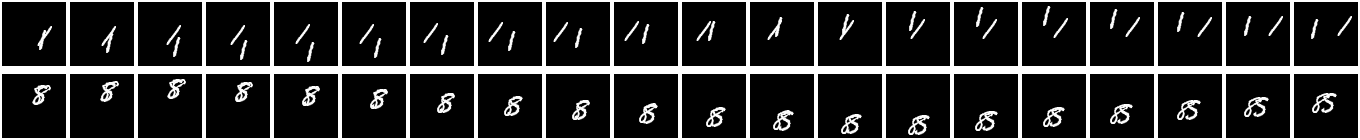
\includegraphics[width=1.0\linewidth]{figures/ds/mm_train.png}
  \caption{Training set}
  \label{fig:mm_train}
  \vspace{.1cm}
\end{subfigure}
\begin{subfigure}{1.0\textwidth}
  \centering
  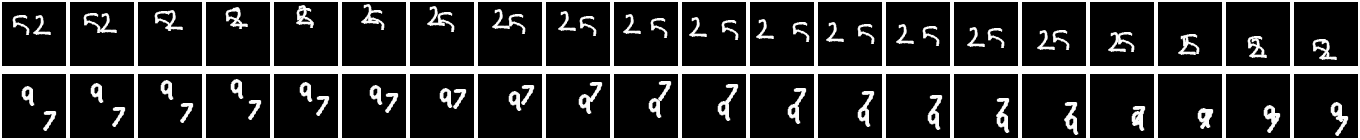
\includegraphics[width=1.0\linewidth]{figures/ds/mm_valid.png}
  \caption{Validation set}
  \label{fig:mm_valid}
  \vspace{.1cm}
\end{subfigure}
\begin{subfigure}{1.0\textwidth}
  \centering
  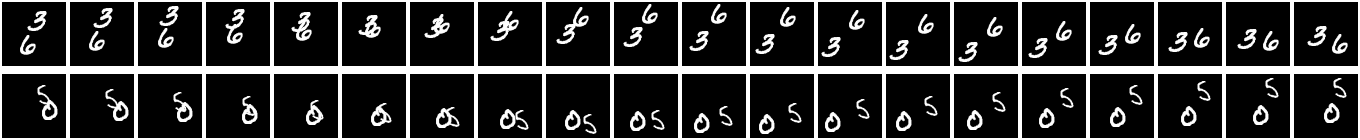
\includegraphics[width=1.0\linewidth]{figures/ds/mm_test.png}
  \caption{Test set}
  \label{fig:mm_test}
\end{subfigure}
\caption[MovingMNIST Image Sequence Samples]{Randomly chosen samples of generated image sequences of size $64 \times 64$ from the Moving MNIST dataset.}
\label{fig:moving_mnist}
\end{figure}

The generation procedure of the validation set is equal to the previously described process to create the training data. But with the difference that the last $5,000$ digits of the original MNIST training split is used. On the contrary, we do not generate the test set on the fly by using the MNIST test split. Instead, we take use of the $10,000$ pre-generate and exaclty $20$ frames long sequences test set used in \parencite{spat_temp_video_autoenc}\footnote{Pre-generated MovingMNIST test set with $10,000$ sequences: \url{http://mi.eng.cam.ac.uk/~vp344/}}. In this way, we are able to achieve more comparable results to at least one competing model. A random sample from each of these splits is presented in Figure \ref{fig:moving_mnist}.

Even that some other works only used a fixed number of pre-generated frame sequences only, we kept up with the on-the-fly generation process of the initial paper for at least three reasons. First, it limits the amound of data and therefore increases the chance of overfitting. Seconds, loading the pre-generated frames from disk takes more time than generating them on the fly; hence it could have a slightly negative impact on the overal performance. And third, it reduces the overall memory requirements in case the whole data would otherwise be pre-loaded into memory in order to eleminate the second mentioned issue.

\subsection{Preprocessing}

Since the original pixel values of the MNIST dataset are in a range of $[0, 255]$, we perform simple rescaling to $[0, 1]$ in order to normalize the data. Futher, we considered to subtract the mean pixel-values as well, because gray-scale images have the stationarity property\footnote{For example when the statistics for each data dimension follows the same distribution, the data is said to be stationary.}. But due to the fact that this is not often done in practice when the MNIST dataset is used \parencite{stanford_data_pre}, as well as we could not see any noticable improvements when applying it, caused that we did not use mean subtraction while preprocessing the data. Moreover, we belief that since most parts of any image is black (and therefore zero), further processing of the data is not necessarily required.

Additionally, instead of feeding the model with continuous floating values in the normalized range, we use binary pixel values only. This decision results from the use of binary cross-entropy as the main loss function, which has shown to be the favourable choice for MNIST image generating models \parencite{unsup_learn_lstm}, \parencite{conv_lstm_nowcasting}. Therefore, we set every pixel $p$ to to zero if $p < 0.5 $, and assign all other pixels a value of one. Moreover, we use sigmoid activation function in the output layer in order to support the saturation of all pixels into either zero or one.

\section{MsPacman}

In order to accommodate the request of assessing our model on more complex data compared to the previously presented Moving MNIST, but which still has negligible dynamics compared to natural clips, we use a second collection of video game recordings. The \textit{MsPacman}\footnote{MsPacman dataset: Generated by \href{mailto:jun_ki_lee@brown.edu}{\textit{Jun Ki Lee}} in a student project at Brown University by taking recording the the classical video game.} dataset has been used in an indepented TensorFlow implementation of \parencite{deep_multiscale_video_pred}\footnote{Adversarial video generation in TensorFlow:\\ \url{https://github.com/dyelax/Adversarial_Video_Generation}} for adversarial video generation and future frame prediction. It contains several interesting dynamics and properties that make it a reasonable choice to be considered in the evaluation of our model. These will be discussed in more detail throughout this section.

\subsection{Characteristics}

The video game dataset contains about half a million single images of size $ 160 \times 210 $. These images can be grouped into \num{517} game recordings for the trainging set and $51$ recordings for the test set. Each recording has a variable length and ranges from about \num{500}-\num{1500} frames per sequence. We take the last \num{51} sequences of the training data for our validation set to have it roughly the same size as the testing set. Thus, we end up with a total number of \num{418287} frames for training, \num{45,007} images for validation and \num{46380} images for testing.

The action inside each recording has a closed world with various game rules that the network has to learn. Just to name some example, all object follow the path between the walls of the game world, with the two exceptions that the ghosts in the center might exit the cave through the top barrier, as well as that Pacman can teleport himself by leaving the world using its left or right exit. Further, the protagonist opens and closes its mouth, can eat the distributed dots, fruits or blue ghosts. Some recordings from the different dataset splits are depicted in Figure \ref{fig:pacman_full}.


\begin{figure}[h!tb]
\centering
\begin{subfigure}{1.0\textwidth}
  \centering
  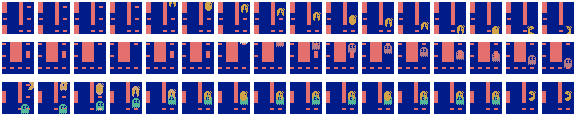
\includegraphics[width=1.0\linewidth]{figures/ds/pac_train.png}
  \caption{Training set}
  \label{fig:pac_train}
  \vspace{.1cm}
\end{subfigure}
\begin{subfigure}{1.0\textwidth}
  \centering
  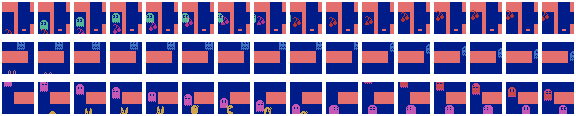
\includegraphics[width=1.0\linewidth]{figures/ds/pac_valid.png}
  \caption{Validation set}
  \label{fig:pac_valid}
  \vspace{.1cm}
\end{subfigure}
\begin{subfigure}{1.0\textwidth}
  \centering
  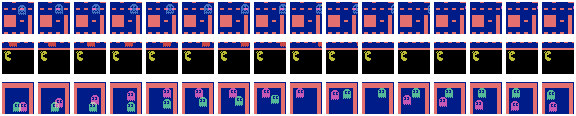
\includegraphics[width=1.0\linewidth]{figures/ds/pac_test.png}
  \caption{Test set}
  \label{fig:pac_test}
\end{subfigure}
\caption[MsPacman Crop Image Samples]{Example sequences from the different splits of the used MsPacman dataset. These randomly selected frames have been to cropped to $32 \times 32 $ and filtered to ensure enough movement while training the model.}
\label{fig:pacman}
\end{figure}


\subsection{Preprocessing and Augmentation} \label{sec:pacman_preprocessing}

We rescaled the images of every sequence to be in range of [-1, 1]. To ensure that the predicted outputs outputs exhibit the same value scale, we use a $tanh$ activation function after the last transposed convolutional layer. Since each single image is quite big, we take advantage from our fully-convolutional approach and train the network on random crops of size $ 32 \times 32 $ only. Some random samples of these cropped images are shown in Figure \ref{fig:pacman}. Unfortunately, the usage of small image crops follows that most of the used training sequences show no motion at all.

After we experienced a strong preference of predicting the worlds background only over the single small moving characters, we decided use a techniqe similar to \parencite{deep_multiscale_video_pred}, in order to ensure that each temporal sequence shows enough movement. Therefore, each time when we select a random part of the sequence from the training set, we calculate the $\ell_2$ difference between each consecutive frames. Afterwards, the interatively reject this randomly chosen crop of the sequence until the the overall movement of the input sequence is higher than a given threshold of $25 \cdot n_{frames}$, or we reach a specified limit in order to prevent an endless loop. Additionally, we ensure that there is also movement at the end of the input sequence to ensure that not the whole movement is just taking place at the beginning of the whole sequence only, as well as to reduce the chance that the network has to predict the movement of newly incoming object only which it obviously cannot predict. Last but not least, we have slightly shortened the input and output sequence length compared to the other two datasets to \num{8} frames each. The reason for this is that the motion detection is kind of useless when being applied on too long sequences, because of the high chance that all these fast moving objects within the selected crop have already left the scene. In particular, before the decoder takes over to predict the future frames. However, even that this filtering of the final training examples sounds quite radical, it is to highlight that a high fraction of the input space is still static content. This can be attributed to the use of convolutional layer with small windows sizes that slide over the whole input space.

In terms of data augmentation, we did \textit{not} randomly modify the brightness or contrast of the image examples, because it does not make sense in context of this video game. But since the game world is mirrored horizontally, we perform random horizontal flipping in case the chosen crop is not showing any parts of the status display at the bottom. Furthermore, we iterated over all sequences \num{256} times per epoch, reasoned by the fact that the dataset consists of only a few but very long sequences. A second reason is that we only use a very small clip and random crop from from these frame sequences. 

\begin{figure}[htpb]
\centering
\begin{subfigure}{1.0\textwidth}
  \centering
  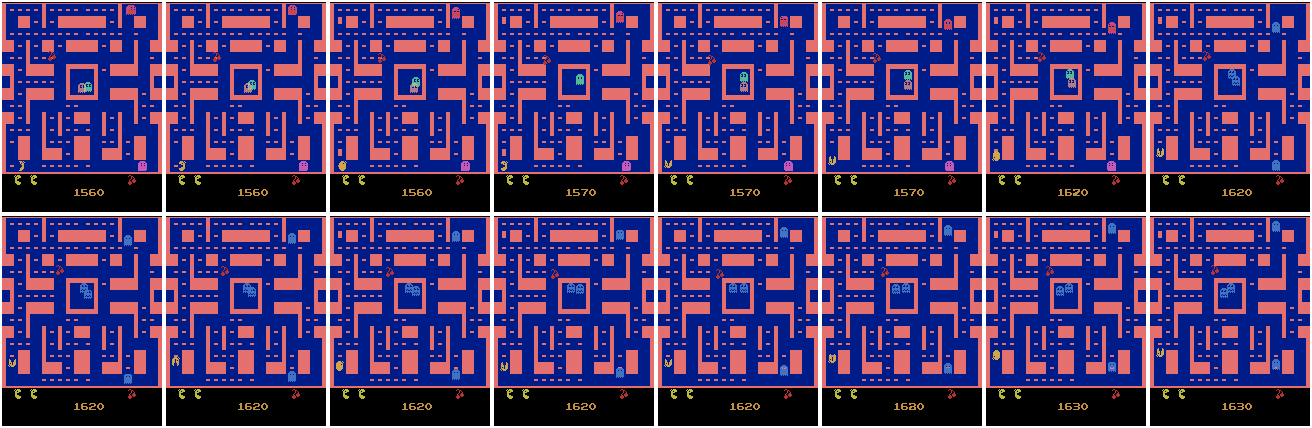
\includegraphics[width=1.0\linewidth]{figures/ds/pac_train_full.png}
  \caption{Training set}
  \label{fig:pac_train_full}
  \vspace{.1cm}
\end{subfigure}
\begin{subfigure}{1.0\textwidth}
  \centering
  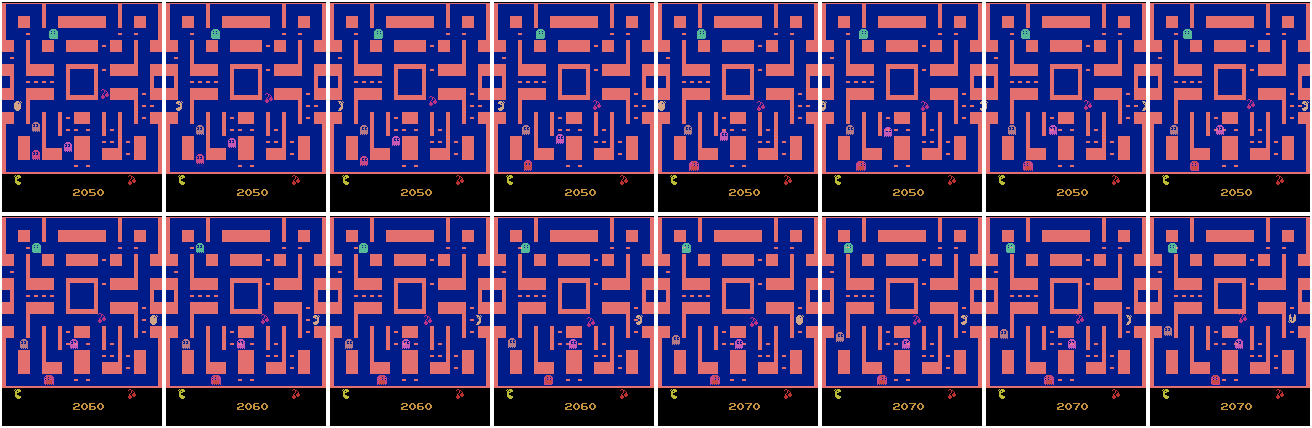
\includegraphics[width=1.0\linewidth]{figures/ds/pac_valid_full.png}
  \caption{Validation set}
  \label{fig:pac_valid_full}
  \vspace{.1cm}
\end{subfigure}
\begin{subfigure}{1.0\textwidth}
  \centering
  \includegraphics[width=1.0\linewidth]{figures/ds/pac_test_full.png}
  \caption{Test set}
  \label{fig:pac_test_full}
\end{subfigure}
\caption[MsPacman Full Image Samples]{Exemplary sequences of game recordings from MsPacman dataset that have been samples randomly from the different splits. Each shown clip has a length of \num{16} frames of size $160 \times 210$.}
\label{fig:pacman_full}
\end{figure}

\section{UCF-101}

Finally, we used a third dataset to examine if our model can also deal with complex, natural videos. Therefore, we use the \textit{UCF-101} dataset \parencite{ucf}\footnote{UCF_101 dataset and further informations: \url{http://crcv.ucf.edu/data/UCF101.php}}. With its \num{13320} clips and about \num{27} hours of video data, it belongs to the largest labeled dataset for human action recognition. The dataset is made of user-uploaded videos that can contain overloaded background or camera movement. All \num{101} categories can divided into \num{25} main groups,  where each video from the same group shares some similar features, such as an rougly equal viewpoint. The action categories can also be seperated into five types, namely human-object interaction, body-motion only, human-human interaction, playing musical instruments and sports. Even that this dataset was originated for human action recogntion, it can be used in context of frame prediction as well by simply using the raw video data only.

Before taking a deeper look into the characteristics and applied preprocessing steps, it is to add that there exists an even larger video dataset for the purpose of video classification or unsupervised learning. This huge dataset is called \textit{Sports-1M} and contains over \num{1.1} million YouTube video links of \num{478} classes that have been annotated in an automated process \parencite{large_video_class}. But due to infrastructural issues with such a huge dataset, as well as a tremendous time exposure regarding data preprocessing, we decided to not use it in this thesis.


\subsection{Characteristics}

The average video length of the whole dataset is about \num{6.2} seconds, while each single can range from about \num{1} second to a maxiumum of \num{71} seconds. Even that the initial paper states that each video has a fixed resulution and frame rate of $ 320 \times 240 $ and \num{25} FPS respectively, we experienced that a handful of videos exhibits a slightly different resolution. Consequently, these frames have been padded with zeros or cropped in the center to end up in an equal size for all videos. Such a padded video, as well as other example clips, can be seen in the first sample of Figure \ref{fig:ucf_valid_full}.

The dataset provides three standards train/test splits intended to be used for either action recognition or action detection. We have chosen the third standard split for action recognition, because it consists of the most videos for training, as well as allowed the simplest divisibility of the test split. Since we expect that a huge training set is fundamental for the network in order deeply explore the inner dynamics, we descide to take the validation data from the test split instead of the training data as usual. For the avoidance of doubt, other previous works using UCF-101 for frame prediction either used only $ 10\% $ of the test set actually for testing \parencite[p. 12]{deep_multiscale_video_pred}, or made no comment about which parts of the data they choose for validation and testing. Finally, we therefore end up with \num{9624}, \num{1232} and \num{2464} videos for the training, validation and test set, respectively.

\begin{figure}[h!tb]
\centering
\begin{subfigure}{1.0\textwidth}
  \centering
  \includegraphics[width=1.0\linewidth]{figures/ds/ucf_train.png}
  \caption{Training set}
  \label{fig:ucf_train}
  \vspace{.1cm}
\end{subfigure}
\begin{subfigure}{1.0\textwidth}
  \centering
  \includegraphics[width=1.0\linewidth]{figures/ds/ucf_valid.png}
  \caption{Validation set}
  \label{fig:ucf_valid}
  \vspace{.1cm}
\end{subfigure}
\begin{subfigure}{1.0\textwidth}
  \centering
  \includegraphics[width=1.0\linewidth]{figures/ds/ucf_test.png}
  \caption{Test set}
  \label{fig:ucf_test}
\end{subfigure}
\caption[UCF-101 Crop Image Samples]{Sequence examples from UCF-101. These frames have been randomly selected from the different splits, cropped to $32 \times 32 $ and filtered to ensure they contain at least a small proportion of motion in it.}
\label{fig:ucf}
\end{figure}

\subsection{Preprocessing and Augmentation}

The data preprocessing that we perform in UCF-101 is very similar to the procedure describe in Section \ref{sec:pacman_preprocessing}, but with the following differences. First, we cut the width and height of all images in half, resulting in downscaled videos of size $160 \times 120$ using linear interpolation. We do this in order to compensate the noisy, pixelated artefacts in the videos. Also, it increases the chance of finding a random crop of size $ 32 \times 32 $ that actually has some true motion in it, instead of just flickering caused by noise. Seconds, we slightly weaken the constraint regarding motion filtering when selecting the crop region of the randomly selected clip. While we still reject a sequence that has a very low motion in the input frames, we do not dismiss miss a sequence that has no motion at the end. Figure \ref{fig:ucf} shows several cropped sequence examples from the different dataset splits that are fed into our model.

Furthermore, because it is wasteful to load the whole video file into memory, especially in regard that only a very small portion of the data is acutally used to generate a single example for the next batch, we perform an additional offline preprocessing of the data before the actual training process starts. For that reason, we iterate over all raw video files and generate non-overlapping binary video sequences with a length of \num{30} frames each. Fortunately, the generated files can be reused after doing this process once. Finally, we end up with \num{55150} clips for the training set, \num{7183} clips for the validation set and \num{14451} clips for the test set.

Regarding data augmentation, we randomly modify the contrast and brightness of the overall image sequence by a delta of $ \pm20\% $, as well as perform random horizonal flipping in the training data. While we do not randomly change the contrast or brightness in the validation or test data, we double their size by using both the normal and flipped instances. Further, we use four crops from every video in each evaluation iteration in order to have a balance between more consistent evaluations and still an acceptable processing time. It is to add that we perform these augmentations on-the-fly. To facilitate this, we use an advanced double-buffered input queue. The first \textit{filename queue} is randomly filled with references to the pre-generated, binary sequence files. Afterward, \num{16} CPU threads enqueue a reference from this queue, load the sequence into memory and then perform all preprocessing steps in parallel, for the purpose of generating a single training example. Finally, this example is then enqueued to the \textit{shuffled batch queue}, from which our model loads its batches from in every iteration. Consequently, there is no waiting time in-between each training step.


\begin{figure}[htpb]
\centering
\begin{subfigure}{1.0\textwidth}
  \centering
  \adjincludegraphics[width=1.0\linewidth,trim={0 {.3333\height} 0 0},clip]{figures/ds/ucf_train_full.png}
  \caption{Training set}
  \label{fig:ucf_train_full}
  \vspace{.1cm}
\end{subfigure}
\begin{subfigure}{1.0\textwidth}
  \centering
  \adjincludegraphics[width=1.0\linewidth,trim={0 0 0 {.3333\height}},clip]{figures/ds/ucf_valid_full.png}
  \caption{Validation set}
  \label{fig:ucf_valid_full}
  \vspace{.1cm}
\end{subfigure}
\begin{subfigure}{1.0\textwidth}
  \centering
  \adjincludegraphics[width=1.0\linewidth,trim={0 0 0 {.3333\height}},clip]{figures/ds/ucf_test_full.png}
  \caption{Test set}
  \label{fig:ucf_test_full}
\end{subfigure}
\caption[UCF-101 Full Image Samples]{Randomly chosen and rescaled clip samples of size $160 \times 120$ from the UCF-101 dataset.}
\label{fig:ucf_full}
\end{figure}


% !TeX root = ../main.tex

% for every dataset-group: tell which loss_main was used by default (if not stated differently)
% tell we use batch_size of 32 always (without any reason...)

% performed on: We implemented our model in TensorFlow v0.10, CUDA 7.5.18 and cuDDN 4.

% explore the model on MovingMNIST (layers, scheduled samling, filter depth)
%      --> fix the main hyper-params
% small grid search on each model?
%      --> compare results

%Wie gehen wir beim Training vor: Wegen sehr vielen Hyperparmeter: Nutzen MM um die einzelnen HParams unanbhängig voneinander zu erforschen. Dann: Grid-Search auf den jeweils besten Einstellungen

\chapter{Evaluation} \label{chapter:evaluation}

This chapter presents the evaluation results of our model on all datasets of chapter \ref{chapter:datasets}. Since the model exhibits a vast number of hyper parameters and each training can take several days, performing an extensive grid search is not possible. That's why we start to explore the model's substantial hyperparameters independently from each other by using the simplest dataset. Afterwards, the acquired knowledge about our model's behavior can then be transfered to the other datasets in order to to a basic grid search. Beside the quantitative assessment of the model, it is also qualitatively compared to experimental results of related projects at the end of each section.

All experiments have been computed on a single Nvidia GeForce GTX Titan X using the TensorFlow open source software library for machine intelligence with version r0.10. This quite new deep learning framework has been developed by Google as a second-generation system based on their experiences on DistBelief \parencite{distbelief}. A computation in TensorFlow is expressed as a statefule dataflow graph, where each node represents a mathematical operation and the graph's edges a data tensor that can flow from one node to the next \parencite{tensorflow2015-whitepaper}. It has gained increasing attention since its first public release in November 2015.

If not stated differently, the model configuration described in Chapter \ref{chapter:implementation} is used, but with a two-layer ConvLSTM using $3\times3$ input-to-hidden and $5\times5$ hidden-to-hidden kernel size in the internal convolutions. Further, we have deactivated the optional BN-layers within these cells for two reasons. Firstly, first tests have not shown any improvements using them. And secondly, the fact that its TensorFlow implementation back then had the issue\footnote{Further details: \url{https://github.com/tensorflow/tensorflow/issues/4361}} of performing batch statistic updates multiple times when being share across time, resulted in an enormous drop in performance. We have therefore kept the use of these batch normalizations of the spatio-temporal encoder and decoder components for future work. Additionally, all weights are initialized using the Xavier method of equation \ref{eq:xavier} and the default weight decay regularization coefficient is set to $\lambda=1e^{-5}$. We use a batch size of 32 during the training process together with Adam optimizer ($\beta_1 = 0.9$, $\beta_2 = 0.999$, $\epsilon =1e^{-8}$) and a default initial learning rate of $\eta = 0.001$. In addition to the learning rate annealing mechanisim of Adam, the learning rate is also manually decreased once per epoch using a stair-case exponential decay function by a factor of $\alpha=0.9$.

Lastly, it has to be menioned that diagrams, which show results of any kind of objective function, are always shown with its y-axis in logarithmic scale so that fine differences become better recognizable. And unless otherwise specified, all losses represent the per-pixel error and averaged across the whole generated future sequence.

\section{Experiments on Moving MNIST} \label{sec:exp-mm}

The synthetic Moving MNIST dataset is used as a starting point for the evaluation of our model. Given an input sequence of ten frames, the network therefore has to understand and encode the motion of this input in order to predict the next ten frames of the future. In this section, we qualitatively and quantitatively compare our results with other network models, because it has been used in several previous works as well. The loss layer used in this section does not use the SSIM term by default.

\subsection{Model Exploration}

The model is incrementally explored in this section in order to understand its behaviour regarding changes in the hyperparameters, as well as to see the effects of the modern techniques used in the training process.

\subsubsection*{Scheduled Sampling}

The consequences of the used scheduled sampling technique is examined first. Figure \ref{fig:plot-mm-asss} visualizes the training and validation binary cross-entropy using our standard model with either scheduled sampling (SS) or always sampling (AS). The latter method means the approach to always sample from the previously generated frame, which is comparable to SS with a constant sampling probability of $p=0$. It can be seen that there is a huge discrepancy between the training and validation error in the starting phase, where the SS-approach mainly trained on input samples taken from the ground truth. The can be explained that sampling on the ground truth in every timestep of the recurrent network tremendously speeds up the convergence of the training loss, because each cell does not have to correct errors of the previous cells. In contrary, the validation loss is very bad in this phase, since the results represent the average out of ten predicted frames and the spatio-temporal decoder suddenly receives its own feature space predictions as input to predict the next frame, which is in contrast to the process while training so far.

\begin{figure}[htb]
  \centering
  \pgfplotstableset{col sep=comma}
  \pgfplotstableread{data/mm/as_ss/run_mm-ss-2l3i5hp-c326464k533s212bn-wd1e-05-YT-tag_validation_bce.csv}\modelA
  \pgfplotstableread{data/mm/as_ss/run_mm-as-2l3i5hp-c326464k533s212bn-wd1e-05-SE-tag_validation_bce.csv}\modelB
  \pgfplotstableread{data/mm/as_ss/run_mm-ss-2l3i5hp-c326464k533s212bn-wd1e-05-YT-tag_loss-BCE_loss-Mean.csv}\modelAA
  \pgfplotstableread{data/mm/as_ss/run_mm-as-2l3i5hp-c326464k533s212bn-wd1e-05-SE-tag_loss-BCE_loss-Mean.csv}\modelBB
  \pgfplotstableread{data/mm/as_ss/run_mm-ss-2l3i5hp-c326464k533s212bn-wd1e-05-YT-tag_scheduled_sampling.csv}\modelSS
  \begin{tikzpicture}
    \begin{axis}[
    	axis y line*=right,
    	hide x axis,
    	ylabel near ticks,
        ymin=0,
        ymax=1,
        xmin=0,
        xmax=65000,
        thick,
        ylabel=GT sampling probability \textit{p},
        xlabel=step \textit{i},
        x post scale=1.8,
      ]
      \addplot[draw=LightGoldenrod, thin, opacity=0.8] table[x=Step, y=Value]{\modelSS};\label{mSS}
    \end{axis}
    \begin{axis}[
    	axis y line*=left,
    	ymode=log,
    	log ticks with fixed point,
        ymin=0,
        ymax=0.3,
        xmin=0,
        xmax=65000,
        ytick={0.05,0.075,0.1,0.15,0.2},
        legend style={legend pos=north east},
        grid,
        thick,
        ylabel=BCE loss,
        xlabel=step \textit{i},
        x post scale=1.8,
      ]
	  \addlegendimage{/pgfplots/refstyle=mSS}\addlegendentry{Scheduled Sampling}    
      
      % background
      \addplot[draw=black!10!blue, thin, opacity=0.8] table[x=Step, y=Value]{\modelBB};
      \addlegendentry{AS (train)}
      \addplot[draw=black!10!green, thin, opacity=0.8] table[x=Step, y=Value]{\modelAA};
      \addlegendentry{SS (train)}
      %foreground
      \addplot[draw=black!30!blue] table[x=Step, y=Value]{\modelB};
      \addlegendentry{AS (valid)}
      %best
      \addplot[draw=black!30!green] table[dashed, x=Step, y=Value]{\modelA};
      \addlegendentry{SS (valid)} 
    \end{axis}
    
  \end{tikzpicture}
  \caption[Influences of Scheduled Sampling]{Influences of scheduled sampling regarding the training and validation error in context of recurrent networks and future frames prediction on Moving MNIST.}\label{fig:plot-mm-asss}
\end{figure}

But the interesting insight here is that as soon as the scheduled sampling component completely changed the input behaviour to inference mode, the achieved prediction performance is continiously better compared to the approach of always sampling from previous generatated frames directly at the very beginning. This behavior could be explained that the SS approach introduces some kind of pre-training phase, where the network can learn to predict the next frame when a perfect current frame is given. Hence, it has not to deal with errors made in the previous time step. By slowly changing this behaviour to the mode as it is used while inference, it then also starts to learn a robustness against imperfect input frames. A similar behavior can be seen when comparing the results of the PSNR metric between AA and SS in Figure \ref{fig:plot-mm-asss2-psnr}. However, when we look at the sharpeness difference metric in Figure \ref{fig:plot-mm-asss2-sdiffcurve}, it can be seen that sharpness of the predictions is continuously better using scheduled sampling.

\begin{figure}[htb]
\centering
\begin{subfigure}{0.5\textwidth}
  \centering
  \pgfplotstableset{col sep=comma}
  \pgfplotstableread{data/mm/as_ss/run_mm-ss-2l3i5hp-c326464k533s212bn-wd1e-05-YT-tag_validation_sharpdiff.csv}\modelA
  \pgfplotstableread{data/mm/as_ss/run_mm-as-2l3i5hp-c326464k533s212bn-wd1e-05-SE-tag_validation_sharpdiff.csv}\modelB
  \hspace*{-0.6cm}
  {
  \begin{tikzpicture}[scale=0.5]
    \begin{axis}[
        ymin=10,
        ymax=15,
        xmin=0,
        xmax=65000,
        legend style={legend pos=south east},
        grid,
        thick,
        ylabel=SharpDiff,
        xlabel=step \textit{i},
        x post scale=1.6,
      ]
      \addplot[draw=black!30!blue] table[x=Step, y=Value]{\modelB};
      \addlegendentry{AS (valid)};
      %best
      \addplot[draw=black!30!green] table[x=Step, y=Value]{\modelA};
      \addlegendentry{SS (valid)};
    \end{axis}
  \end{tikzpicture}
  }
  \caption{}
  \label{fig:plot-mm-asss2-sdiffcurve}
\end{subfigure}%
\begin{subfigure}{0.5\textwidth}
  \centering
  \pgfplotstableset{col sep=comma}
  \pgfplotstableread{data/mm/as_ss/run_mm-ss-2l3i5hp-c326464k533s212bn-wd1e-05-YT-tag_validation_psnr.csv}\modelA
  \pgfplotstableread{data/mm/as_ss/run_mm-as-2l3i5hp-c326464k533s212bn-wd1e-05-SE-tag_validation_psnr.csv}\modelB
  \hspace*{-0.6cm}
  {
  \begin{tikzpicture}[scale=0.5]
    \begin{axis}[
        ymin=10,
        ymax=20,
        xmin=0,
        xmax=65000,
        legend style={legend pos=south east},
        grid,
        thick,
        ylabel=PSNR,
        xlabel=step \textit{i},
        x post scale=1.6,
      ]
      \addplot[draw=black!30!blue] table[x=Step, y=Value]{\modelB};
      \addlegendentry{AS (valid)};
      %best
      \addplot[draw=black!30!green] table[x=Step, y=Value]{\modelA};
      \addlegendentry{SS (valid)};
    \end{axis}
  \end{tikzpicture}
  }
  \caption{}
  \label{fig:plot-mm-asss2-psnr}
\end{subfigure}
\caption[Image Metrics Comparing AS and SS]{Comparison of validation results based on a model with either using the scheduled sampling or the always sampling training technique.} \label{fig:plot-mm-asss2}
\end{figure}



\subsubsection*{Batch Normalization}

The use of batch normalization in the spatial encoder and decoder components is investigated next. Figure \ref{fig:plot-mm-bn} shows a clear advantage of using BN-layers. It can be argued that our model is able to profit strongly from  batch normalization, because it does not only support the convolutional encoder and decoder to learn faster by compensating the internal covariate shift. Also, both recurrent networks in-between can benefit from this, reasoned by the fact that the frame representations in feature space, that are produced by the spatial encoders, tend to have a more stable distribution. Consequently, the spatio-temporal encoder has fewer problems to extract useful patterns from these representations while consuming them in the course of the training process.

\begin{figure}[htb]
\centering
\begin{subfigure}{0.5\textwidth}
  \centering
  \pgfplotstableset{col sep=comma}
  \pgfplotstableread{data/mm/bn/run_mm-ss-2l3i5hp-c326464k533s212bn-wd1e-05-XG-tag_validation_bce.csv}\modelA
  \pgfplotstableread{data/mm/bn/run_mm-ss-2l3i5hp-c326464k533s212-wd1e-05-MX-tag_validation_bce.csv}\modelB
  \hspace*{-0.6cm}
  {
  \begin{tikzpicture}[scale=0.5]
    \begin{axis}[
        ymode=log,
    	log ticks with fixed point,
        ymin=0,
        ymax=0.3,
        xmin=0,
        xmax=65000,
        legend style={legend pos=north east},
        grid,
        thick,
        ylabel=BCE loss,
        xlabel=step \textit{i},
        x post scale=1.6,
      ]
      \addplot[draw=black!30!blue] table[x=Step, y=Value]{\modelB};
      \addlegendentry{w/o BN (valid)};
      %best
      \addplot[draw=black!30!green] table[x=Step, y=Value]{\modelA};
      \addlegendentry{with BN (valid)};
    \end{axis}
  \end{tikzpicture}
  }
  \caption{}
  \label{fig:plot-mm-bn-bce}
\end{subfigure}%
\begin{subfigure}{0.5\textwidth}
  \centering
  \pgfplotstableset{col sep=comma}
  \pgfplotstableread{data/mm/bn/run_mm-ss-2l3i5hp-c326464k533s212bn-wd1e-05-XG-tag_validation_sharpdiff.csv}\modelA
  \pgfplotstableread{data/mm/bn/run_mm-ss-2l3i5hp-c326464k533s212-wd1e-05-MX-tag_validation_sharpdiff.csv}\modelB
  \hspace*{-0.6cm}
  {
  \begin{tikzpicture}[scale=0.5]
    \begin{axis}[
        ymin=10,
        ymax=15,
        xmin=0,
        xmax=65000,
        legend style={legend pos=south east},
        grid,
        thick,
        ylabel=SharpDiff,
        xlabel=step \textit{i},
        x post scale=1.6,
      ]
      \addplot[draw=black!30!blue] table[x=Step, y=Value]{\modelB};
      \addlegendentry{w/o BN (valid)};
      %best
      \addplot[draw=black!30!green] table[x=Step, y=Value]{\modelA};
      \addlegendentry{with BN (valid)};
    \end{axis}
  \end{tikzpicture}
  }
  \caption{}
  \label{fig:plot-mm-bn-psnr}
\end{subfigure}
\caption[Influences of Batch Normalization]{Comparison of the validation results from two model instances where one uses batch normalization layers in the spatial encoder and decoder components.} \label{fig:plot-mm-bn}
\end{figure}


\subsubsection*{Learning Rate Decay}

The network's learning behavior using two different exponential decay rates is illustrated in Figure \ref{fig:plot-mm-lr}. In this example, the learning rate is slightly decayed after each epoch by a specified factor. Because the Moving MNIST dataset is generated on-the-fly, we specify its total size to be virtually \num{32000}. In this way, the learning rate is effectively decayed after each validation step\footnote{In the course of this evaluation, we assess our model in a full epoch on the validation set every \nth{1000} training step.}, since a batch size of \num{32} is used. The network denoted with blue has a clear disadvantage, because its learning rate at the end became so small that it alsmost stops learning. However, throughout our experiments we determined that a very low learning rate at the end of the training was beneficial regarding the image quality and finer details of the generated images.

\begin{figure}[htb]
  \centering
  \pgfplotstableset{col sep=comma}
  \pgfplotstableread{data/mm/lr/run_mm-ss-2l3i5hp-c326464k533s212bn-wd1e-05-JK-tag_validation_bce.csv}\modelA
  \pgfplotstableread{data/mm/lr/run_mm-ss-2l3i5hp-c326464k533s212bn-wd1e-05-XG-tag_validation_bce.csv}\modelB
  \pgfplotstableread{data/mm/lr/run_mm-ss-2l3i5hp-c326464k533s212bn-wd1e-05-JK-tag_learning_rate.csv}\modelLrA
  \pgfplotstableread{data/mm/lr/run_mm-ss-2l3i5hp-c326464k533s212bn-wd1e-05-XG-tag_learning_rate.csv}\modelLrB
  \begin{tikzpicture}
    \begin{axis}[
    	axis y line*=right,
    	hide x axis,
    	ylabel near ticks,
        ymin=0,
        ymax=0.001,
        xmin=0,
        xmax=65000,
        thick,
        ylabel={Learning rate $\eta$},
        xlabel=step \textit{i},
        x post scale=1.8,
      ]
      \addplot[draw=black!10!blue, very thin, opacity=0.8] table[x=Step, y=Value]{\modelLrB};\label{mB}
      \addplot[draw=black!10!green, very thin, opacity=0.8] table[x=Step, y=Value]{\modelLrA};\label{mA}
    \end{axis}
    \begin{axis}[
    	axis y line*=left,
    	ymode=log,
    	log ticks with fixed point,
        ymin=0,
        ymax=0.3,
        xmin=0,
        xmax=65000,
        ytick={0.05,0.075,0.1,0.15,0.2},
        legend style={legend pos=north east},
        grid,
        thick,
        ylabel=BCE loss,
        xlabel=step \textit{i},
        x post scale=1.8,
      ]
	  \addlegendimage{/pgfplots/refstyle=mB}\addlegendentry{$\eta$-decay=0.90 (valid)}
      \addlegendimage{/pgfplots/refstyle=mA}\addlegendentry{$\eta$-decay=0.95 (valid)}
      
      %foreground
      \addplot[draw=black!30!blue] table[x=Step, y=Value]{\modelB};
      \addlegendentry{$\eta$-decay=0.90};
      %best
      \addplot[draw=black!30!green] table[dashed, x=Step, y=Value]{\modelA};
      \addlegendentry{$\eta$-decay=0.90};
    \end{axis}
  \end{tikzpicture}
  \caption[Influences of Learning Rate Decay]{Validation losses of two identical network models using different learning rate decay rates in combination with Adam optimizer.}\label{fig:plot-mm-lr}
\end{figure}


\subsubsection*{ConvLSTM Feature Maps}

Next, we investigate the network's behavior with respect to the hidden-to-hidden feature maps in the spatio-temporal decoder and encoder components. Therefore, we adjust the number of feature maps produced by the convolutional layers in the spatial encoder. While a first simpler variant is used that produces (16, 32, 32) feature maps in each layer, another more complex variant is used as well which convolves (64, 128, 128) feature maps. The number feature maps produced by the last layer is then used constantly within the ConvLSTM cells and its temporal transitions. Consequently, the performance of these two model configurations is compared against the standard model with 64 temporal feature maps in Figure \ref{fig:plot-mm-filter}.

\begin{figure}[htb]
\centering
\begin{subfigure}{0.5\textwidth}
  \centering
  \pgfplotstableset{col sep=comma}
  \pgfplotstableread{data/mm/filters/run_mm-ss-2l3i5hp-c326464k533s212bn-wd1e-04-FG-tag_validation_bce.csv}\modelA
  \pgfplotstableread{data/mm/filters/run_mm-ss-2l3i5hp-c163232k533s212bn-wd1e-04-YP-tag_validation_bce.csv}\modelB
  \pgfplotstableread{data/mm/filters/run_mm-ss-2l3i5hp-c64128128k533s212bn-wd1e-05-NK-tag_validation_bce.csv}\modelC
  \hspace*{-0.6cm}
  {
  \begin{tikzpicture}[scale=0.5]
    \begin{axis}[
        ymode=log,
    	log ticks with fixed point,
        ymin=0,
        ymax=0.3,
        xmin=0,
        xmax=65000,
        ytick={0.05,0.075,0.1,0.15,0.2},
        legend style={legend pos=north east},
        grid,
        thick,
        ylabel=BCE loss,
        xlabel=step \textit{i},
        x post scale=1.6,
      ]
      \addplot[draw=black!30!blue] table[x=Step, y=Value]{\modelB};
      \addlegendentry{32 feature maps (valid)};
      %best
      \addplot[draw=black!30!green] table[x=Step, y=Value]{\modelA};
      \addlegendentry{64 feature maps (valid)};
      
      \addplot[draw=black!30!red] table[x=Step, y=Value]{\modelC};
      \addlegendentry{128 feature maps (valid)};
    \end{axis}
  \end{tikzpicture}
  }
  \caption{}
  \label{fig:plot-mm-filter-bce}
\end{subfigure}%
\begin{subfigure}{0.5\textwidth}
  \centering
  \pgfplotstableset{col sep=comma}
  \pgfplotstableread{data/mm/filters/run_mm-ss-2l3i5hp-c326464k533s212bn-wd1e-04-FG-tag_validation_ssim.csv}\modelA
  \pgfplotstableread{data/mm/filters/run_mm-ss-2l3i5hp-c163232k533s212bn-wd1e-04-YP-tag_validation_ssim.csv}\modelB
  \pgfplotstableread{data/mm/filters/run_mm-ss-2l3i5hp-c64128128k533s212bn-wd1e-05-NK-tag_validation_ssim.csv}\modelC
  \hspace*{-0.6cm}
  {
  \begin{tikzpicture}[scale=0.5]
    \begin{axis}[
        ymin=0.5,
        ymax=1.0,
        xmin=0,
        xmax=65000,
        legend style={legend pos=south east},
        grid,
        thick,
        ylabel=SSIM,
        xlabel=step \textit{i},
        x post scale=1.6,
      ]
      \addplot[draw=black!30!blue] table[x=Step, y=Value]{\modelB};
      \addlegendentry{32 feature maps};
      %best
      \addplot[draw=black!30!green] table[x=Step, y=Value]{\modelA};
      \addlegendentry{64 feature maps};
      
      \addplot[draw=black!30!red] table[x=Step, y=Value]{\modelC};
      \addlegendentry{128 feature maps};
    \end{axis}
  \end{tikzpicture}
  }
  \caption{}
  \label{fig:plot-mm-filter-psnr}
\end{subfigure}
\caption[Influences of ConvLSTM Feature Maps]{Impact of the number of feature maps within the ConvLSTM encoder and decoder networks regarding overall frame prediction performance.} \label{fig:plot-mm-filter}
\end{figure}

As expected, the network with only 32 feature maps performs worse compared to the standard setting. But it is very surprising that the model configuration with 128 feature maps achieves even worse results. One possible reason could be a unfavorable, random initialization of the initial model parameters. However, due to the fact that such a network configuration requires roughly the entire video memory of the GPU, as well as takes twice as long to train, we came to the decision to continue our experiments on 64 feature maps only.


\subsubsection*{ConvLSTM Layers}

The number of recurrent layers has a very positive effect in order to generate future frames of better quality. The same behavior has also been mentioned in the practical experiment of \parencite[p. 6]{unsup_learn_lstm}, where they have qualitatively shown that a deeper LSTM is able to generate sharper images. Figure \ref{fig:plot-mm-layer} shows that the improvements of adding a third layer is apparently smaller compared to the difference when a second layer is added. Unfortunately, a 4-layer network could not be tested due to memory limitations of the graphics card. Additionally, it is worthwhile noting that the number of recurrent layers has a huge impact in respect to model complexity, training time and memory requirements.

\begin{figure}[htb] % note: these use triplet loss already!!!
\centering
\begin{subfigure}{0.5\textwidth}
  \centering
  \pgfplotstableset{col sep=comma}
  \pgfplotstableread{data/mm/layers/run_mm-ss-3l3i5hp-c326464k533s212bn-wd1e-05-triplet-JM-tag_validation_bce.csv}\modelA
  \pgfplotstableread{data/mm/layers/run_mm-ss-2l3i5hp-c326464k533s212bn-wd1e-05-triplet-CE-tag_validation_bce.csv}\modelB
  \pgfplotstableread{data/mm/layers/run_mm-ss-1l3i5hp-c326464k533s212bn-wd1e-05-triplet-MK-tag_validation_bce.csv}\modelC
  \hspace*{-0.6cm}
  {
  \begin{tikzpicture}[scale=0.5]
    \begin{axis}[
    	ymode=log,
    	log ticks with fixed point,
        ymin=0,
        ymax=0.3,
        xmin=0,
        xmax=65000,
        ytick={0.05,0.075,0.1,0.15,0.2},
        legend style={legend pos=north east},
        grid,
        thick,
        ylabel=BCE loss,
        xlabel=step \textit{i},
        x post scale=1.6,
      ]
      \addplot[draw=black!30!red] table[x=Step, y=Value]{\modelC};
      \addlegendentry{1-layer ConvLSTM};
      \addplot[draw=black!30!blue] table[x=Step, y=Value]{\modelB};
      \addlegendentry{2-layer ConvLSTM};
      %best
      \addplot[draw=black!30!green] table[x=Step, y=Value]{\modelA};
      \addlegendentry{3-layer ConvLSTM};
    \end{axis}
  \end{tikzpicture}
  }
  \caption{}
  \label{fig:plot-mm-layer-bce}
\end{subfigure}%
\begin{subfigure}{0.5\textwidth}
  \centering
  \pgfplotstableset{col sep=comma}
  \pgfplotstableread{data/mm/layers/run_mm-ss-3l3i5hp-c326464k533s212bn-wd1e-05-triplet-JM-tag_validation_psnr.csv}\modelA
  \pgfplotstableread{data/mm/layers/run_mm-ss-2l3i5hp-c326464k533s212bn-wd1e-05-triplet-CE-tag_validation_psnr.csv}\modelB
  \pgfplotstableread{data/mm/layers/run_mm-ss-1l3i5hp-c326464k533s212bn-wd1e-05-triplet-MK-tag_validation_psnr.csv}\modelC
  \hspace*{-0.6cm}
  {
  \begin{tikzpicture}[scale=0.5]
    \begin{axis}[
        ymin=10,
        ymax=20,
        xmin=0,
        xmax=65000,
        legend style={legend pos=south east},
        grid,
        thick,
        ylabel=PSNR,
        xlabel=step \textit{i},
        x post scale=1.6,
      ]
      \addplot[draw=black!30!red] table[x=Step, y=Value]{\modelC};
      \addlegendentry{1-layer ConvLSTM};
      \addplot[draw=black!30!blue] table[x=Step, y=Value]{\modelB};
      \addlegendentry{2-layer ConvLSTM};
      %best
      \addplot[draw=black!30!green] table[x=Step, y=Value]{\modelA};
      \addlegendentry{3-layer ConvLSTM};
    \end{axis}
  \end{tikzpicture}
  }
  \caption{}
  \label{fig:plot-mm-layer-psnr}
\end{subfigure}
\caption[Influences of ConvLSTM Layers]{Validation performance of network models with a varying number of recurrent layers. All three models are trained using the triplet loss function.} \label{fig:plot-mm-layer}
\end{figure}



\subsubsection*{Loss Layer}

As a last experiment of our test series, we examine the impact of the different loss terms. Three networks with the identical standard configurations, but different objective functions have therefore been trained. Starting from a network using binary cross-entropy only, perceptual motivated loss terms like GDL and SSIM are added one after another until we end up in the triplet loss described in equation \ref{eq:triplet}. The validation results are depicted in Figure \ref{fig:plot-mm-loss}.

\begin{figure}[htb]
\centering
\begin{subfigure}{0.5\textwidth}
  \centering
  \pgfplotstableset{col sep=comma}
  \pgfplotstableread{data/mm/loss/run_mm-ss-2l3i5hp-c326464k533s212bn-wd1e-05-mae_only-HE,tag_validation_bce.csv}\modelA
  \pgfplotstableread{data/mm/loss/run_mm-ss-2l3i5hp-c326464k533s212bn-wd1e-05-JK,tag_validation_bce.csv}\modelB
  \pgfplotstableread{data/mm/loss/run_mm-ss-2l3i5hp-c326464k533s212bn-wd1e-05-triplet-CE,tag_validation_bce.csv}\modelC
  \hspace*{-0.6cm}
  {
  \begin{tikzpicture}[scale=0.5]
    \begin{axis}[
        ymode=log,
    	log ticks with fixed point,
        ymin=0,
        ymax=0.3,
        xmin=0,
        xmax=65000,
        legend style={legend pos=north east},
        grid,
        thick,
        ylabel=BCE loss,
        xlabel=step \textit{i},
        x post scale=1.6,
      ]
      \addplot[draw=black!30!red] table[x=Step, y=Value]{\modelC};
      \addlegendentry{BCE+GDL+SSIM (valid)};
      \addplot[draw=black!30!blue] table[x=Step, y=Value]{\modelB};
      \addlegendentry{BCE+GDL (valid)};
      %best
      \addplot[draw=black!30!green] table[x=Step, y=Value]{\modelA};
      \addlegendentry{BCE (valid)};
    \end{axis}
  \end{tikzpicture}
  }
  \caption{}
  \label{fig:plot-mm-loss-bce}
\end{subfigure}%
\begin{subfigure}{0.5\textwidth}
  \centering
  \pgfplotstableset{col sep=comma}
  \pgfplotstableread{data/mm/loss/run_mm-ss-2l3i5hp-c326464k533s212bn-wd1e-05-mae_only-HE,tag_validation_sharpdiff.csv}\modelA
  \pgfplotstableread{data/mm/loss/run_mm-ss-2l3i5hp-c326464k533s212bn-wd1e-05-JK,tag_validation_sharpdiff.csv}\modelB
  \pgfplotstableread{data/mm/loss/run_mm-ss-2l3i5hp-c326464k533s212bn-wd1e-05-triplet-CE,tag_validation_sharpdiff.csv}\modelC
  \hspace*{-0.6cm}
  {
  \begin{tikzpicture}[scale=0.5]
    \begin{axis}[
        ymin=10,
        ymax=15,
        xmin=0,
        xmax=65000,
        legend style={legend pos=south east},
        grid,
        thick,
        ylabel=SharpDiff,
        xlabel=step \textit{i},
        x post scale=1.6,
      ]
      \addplot[draw=black!30!red] table[x=Step, y=Value]{\modelC};
      \addlegendentry{BCE+GDL+SSIM (valid)};
      \addplot[draw=black!30!blue] table[x=Step, y=Value]{\modelB};
      \addlegendentry{BCE+GDL (valid)};
      %best
      \addplot[draw=black!30!green] table[x=Step, y=Value]{\modelA};
      \addlegendentry{BCE (valid)};
    \end{axis}
  \end{tikzpicture}
  }
  \caption{}
  \label{fig:plot-mm-loss-psnr}
\end{subfigure}
\caption[Influences of the Loss Term]{Comparison of the validation loss using different objective functions.} \label{fig:plot-mm-loss}
\end{figure}

While the network purely trained on the BCE loss function performs best regarding the binary cross-entropy on the validation set, it nevertheless performs worst according to the sharpness difference metric shown in Figure \ref{fig:plot-mm-loss-psnr}. These results are not surprising, because network using a the triplet loss function for example is putting more emphisis on other properties, in contrast to specifically optimizing it regarding to the binary cross-entropy. However, after we have qualitatively analyzed many generated prediction samples in the course of our experiments, we had the impression that results using the simple BCE loss produced the best results. Especially in samples where one handwritten number crosses the other number, the predictions multiple time steps afterwards kept slightly more stable. All in all, perceptual motivated loss terms seem to be useless or even slightly counter-productive when applied on binary Moving MNIST image frames. 

\subsection{Results}

For the final evaluation of our model with Moving MNIST, we assess the qualitativ and quantitative performance of the best configuration on the test set. Inspired by the findings of our model exploration, as well a rudimentary grid-search, the model for this final test ends up to use the default settings as described earlier, but with an exponential learning rate decay of $\alpha=0.95$ and a loss layer that utilizes no perceptual motivated loss term. We have trained three models of this network with different numbers of recurrent layers for \num{100000} steps.


\subsubsection{Quantitative Results}

A comparison of our best performing model with experimental results of other works is given in Table \ref{tab:mm-comparison}. It can be seen that our model exhibits way less model parameters, especially compared to FC-LSTM approaches. Nevertheless, our ConvLSTM model is able to cut the average pixel-wise test error of the best performing competitive model in halves. The listed results are taken from several published papers. However, we were not able to reproduce the results of FC-LSTM-Combo published in \parencite{unsup_learn_lstm} using their open-source code. After training the model for about \num{1000000} training steps, which took almost one week, the results were not nearly as good as in the paper. Even about \num{20000} training iterations are already sufficient for our model to generate better results.

\begin{table}[htb]
  \small
  \centering
  \begin{tabular}{l r r}
    \toprule
      \textbf{Model} & \textbf{Trainable parameters} & \textbf{BCE test error} \\
    \midrule
      FC-LSTM-Combo(2048-2048) \tiny{\parencite{unsup_learn_lstm}} & \num{214001664} & 0.0855 \\
      FC-LSTM(2048-2048) \tiny{\parencite{conv_lstm_nowcasting}} & \num{142667776} & 0.1180 \\
      ConvLSTM(5/128-64-64) \tiny{\parencite{conv_lstm_nowcasting}} & \num{7585296} & 0.0896 \\
      2enc-ConvLSTM(7/45-45)\footnote{Single frame prediction result, not the average error ofall 10 predicted future frames.} \tiny{\parencite{spat_temp_video_autoenc}} & \num{6132203} & 0.0835 \\
    \midrule
      3enc-ConvLSTM-SS-3dec(5/64) & \num{1841793} & 0.0524 \\
      3enc-ConvLSTM-SS-3dec(5/64-64) & \num{3570817} & 0.0414 \\
      3enc-ConvLSTM-SS-3dec(5/64-64-64) & \num{1} & \\ %TODO
    \bottomrule
  \end{tabular}
  \caption[Results on Moving MNIST]{Comparison with other networks on Moving MNIST. The numbers in brackets identify the \textit{amount of hidden units} per layer in case of FC-LSTMs, and for ConvLSTMs the \textit{hidden-to-hidden kernel size} followed by the \textit{feature maps per layer} are listed. Further, \textit{3enc} denotes tree convolutional layers in the spatial encoder. We call our model 3enc-ConvLSTM-SS-3dec.}\label{tab:mm-comparison}
\end{table}

\subsubsection{Qualitative Results}

Next, several future frame prediction samples are qualitatively compared with results of other models presented earlier in chapter \ref{chapter:relatedwork}. To that end, we take all Moving MNIST examples that are published in other works and apply our network on exactly the same input data. The contrast against an FC-LSTM approach can be seen in Figures \ref{fig:mm-pred-spec-lstm1} or \ref{fig:mm-pred-spec-lstm1}, as well as the comparison with another ConvLSTM implementation in Figure \ref{fig:mm-pred-spec2-clstm1}. The outcomes of our two-layer model are slightly sharper and much brighter in all three examples. However, the digits \num{3} and \num{0} in Figure \ref{fig:mm-pred-spec-lstm} show some visible artifacts at the end of the predicted future sequence.

\begin{figure}[h!tb]
\centering
\begin{subfigure}{0.49\textwidth}
  \centering
  \includegraphics[width=0.92\linewidth]{figures/pred/mm/spec/prediction-00.png}
  \caption{}
  \label{fig:mm-pred-spec-lstm1}
\end{subfigure}%
\begin{subfigure}{0.49\textwidth}
  \centering
  \includegraphics[width=0.92\linewidth]{figures/pred/mm/spec/prediction-01.png}
  \caption{}
  \label{fig:mm-pred-spec-lstm2}
\end{subfigure}
\begin{subfigure}{0.49\textwidth}
  \centering
  \includegraphics[width=0.92\linewidth]{figures/pred/mm/spec/prediction-02.png}
  \caption{}
  \label{fig:mm-pred-spec-lstm3}
\end{subfigure}
\begin{subfigure}{0.49\textwidth}
  \centering
  \includegraphics[width=0.92\linewidth]{figures/pred/mm/spec/prediction-03.png}
  \caption{}
  \label{fig:mm-pred-spec-lstm4}
\end{subfigure}
\caption[Comparison with LSTM on Moving MNIST]{Qualitative comparison with FC-LSTM-Combo(2048-2048) \parencite{unsup_learn_lstm}. Experiments in (c) and (d) are using a different number of digits than the network was trained for. From top to bottom: inputs sequence; ground truth target sequence; predictions of FC-LSTM-Combo, predictions of our 2-layer model.} \label{fig:mm-pred-spec-lstm}
\end{figure}

Further predictions of our model, which have been randomly chosen from the Moving MNIST test set, can be found in Figure \ref{fig:mm-pred-random} in the appendix. While most generated results look quite similar to the ground truth future, the sample in Figure \ref{fig:mm-pred-random2} clearly shows that the model still has its issues to preserve details when both digits overlap each other over a longer period.


\subsubsection{Out-of-Domain Results}

Additionally, we verify the model's ability to deal with data that is outside the domain it has been trained for. We therefore take several Moving MNIST sequences that use one or three digits instead of two and compare the generated results with predictions generated by other competitive models. At this point, it is to highlight that we are not just cherry-picking the best generated predictions in this experiment, because we take the exact same sequences that have been used in related works. In a manner of speaking, we are probably using input sequences where other network models have performed best.

\begin{figure}[h!tb]
\centering
\begin{subfigure}{0.49\textwidth}
  \centering
  \includegraphics[width=0.92\linewidth]{figures/pred/mm/spec/prediction-04.png}
  \caption{}
  \label{fig:mm-pred-spec2-clstm1}
\end{subfigure}%
\begin{subfigure}{0.49\textwidth}
  \centering
  \includegraphics[width=0.92\linewidth]{figures/pred/mm/spec/prediction-05.png}
  \caption{}
  \label{fig:mm-pred-spec2-clstm2}
\end{subfigure}
\caption[Comparison with other ConvLSTM on Moving MNIST]{Qualitative comparison with ConvLSTM(5/128-64-64 \parencite{conv_lstm_nowcasting}. The experiment in (b) uses more digits than the network was trained for. From top to bottom: inputs sequence; ground truth target sequence; prediction results of the competitive model, predictions of our 2-layer ConvLSTM.} \label{fig:mm-pred-spec2-clstm}
\end{figure}

A remarkable difference is visible when the outcames of our model is qualitatively compared with predictions of existing approaches. In case of the samples using three digits in Figures \ref{fig:mm-pred-spec-lstm4} and \ref{fig:mm-pred-spec2-clstm2}, the structure of each digit stays more stable and does not get washed-out, even after a digit has been overlapped by both others. Moreover, it does not try to merge two numbers in order to end up with the same number of digits like the networks have been trained for. A similar behaviour can be seen in Figure \ref{fig:mm-pred-spec-lstm3}, where only a single digit is used. In that scenario, the other network model cearly tries to hallucinate a second fyling number at the end of the future sequence. This misbehavior is not visible in the outputs of our model.

Futher out-of-domain results can be found in Figure \ref{fig:mm-pred-long} in the appendix. It shows the scenario where our model tries to predict a much longer sequence than it has been trained for. Such a scenario is very to realize with our model due to its recurrent encoder-decoder architecture. We therefore unroll the spatio-temporal decoder component for \num{30} time steps in order to verify the long-term stability of the predicted frames. It can be seen that the network is able to continuously produce acceptable results, with the exception of the last five frame in Figure \ref{fig:mm-pred-long1}. From about the \nth{30} predicted future frame, our model then starts to produce very noisy outcomes in almost every case.


\section{Experiments on MsPacman} \label{sec:exp-pac}

The network model is applied on the MsPacman dataset in our second experiment to see how it behaves with data of increased complexity. The effects of perceptual motivated loss terms are investigated more deeply in this dataset, because we strongly belief that their weaknesses in Section \ref{sec:exp-mm} are cause by the unnaturally of binary image data.


\subsection{Hyperparamter Tuning}

In order to find good hyperparameters for the network model, we started to use the best performing model of Moving MNIST, but with the four modifications. First, the three layers of the spatial encoder and decoder components are using strides of $s_i=(1, 2, 1)$ instead $s_i=(2, 1, 2)$, where $i$ denotes the index of the convolutional layer, in order to end up with a feature space representation of the same shape as before. This change is is caused by the fact that the model is trained on smaller $32 \times 32$ patches. Second, we use a \textit{tanh} activation function in the output layer so that each generated frame is within the valid scale. Third, a learning rate decay of $\alpha=0.95$ per epoch is used by default. And lastly, the triplet loss function of Section \ref{sec:impl-components} with MAE as the main loss function is used as a starting point in this evaluation, because previous works have shown its advantages in image processing tasks compared to squared error.

We trained several networks with different numbers of recurrent layers, varying initial learning rates $\eta \in \{0.0005, 0.001, 0.005\}$, as well as different weight decays $\lambda \in \{1e^{-6}, 1e^{-5}, 1e^{-4}\} $. While we could see a clear imrovement between the single layer and two-layer ConvLSTM model, there has been no clear benefit from using a third layer. The differences in results when we performed variations in learning rate and weight decay have also been marginal. Eventaully, we ended up with an initial learning rate of $\eta = 0.0005 $ and continued to use the default weight decay of $\lambda = 1e^{-5}$. Further, we used the two-layer model with the main reason to save training time.


\subsubsection*{Loss Layer}

Even that we couldn't improve our network's performance by performing variations in several hyperparameters that much, we experienced that variations in the objective function could caused more noticeable differences in both quantitativ and qualitative results. As a consequence, we descided to do a further investigation by using different loss terms. Severals validation results are therefore illustrated in Figure \ref{fig:plot-pac-loss}. 

\begin{figure}[htb]
\centering
\begin{subfigure}{0.5\textwidth}
  \centering
  \pgfplotstableset{col sep=comma}
  \pgfplotstableread{data/pac/loss/mse/run_pac-ss-2l3i5hp-c326464k533s121bn-wd1e-05-mse-triplet-MZ_validation_mse.csv}\modelA
  \pgfplotstableread{data/pac/loss/mse/run_pac-ss-2l3i5hp-c326464k533s121bn-wd1e-05-mse-QQ_validation_mse.csv}\modelB
  \pgfplotstableread{data/pac/loss/mse/run_pac-ss-2l3i5hp-c326464k533s121bn-wd1e-05-mae-triplet-VY_validation_mse.csv}\modelC
  \pgfplotstableread{data/pac/loss/mse/run_pac-ss-2l3i5hp-c326464k533s121bn-wd1e-05-mae-LU_validation_mse.csv}\modelD
  \hspace*{-0.6cm}
  {
  \begin{tikzpicture}[scale=0.5]
    \begin{axis}[
        ymode=log,
    	log ticks with fixed point,
        ymin=0,
        ymax=0.3,
        xmin=0,
        xmax=100000,
        legend style={legend pos=north east},
        grid,
        thick,
        ylabel=MSE loss,
        xlabel=step \textit{i},
        x post scale=1.6,
      ]
      \addplot[draw=black!30!orange] table[x=Step, y=Value]{\modelD};
      \addlegendentry{MAE+GDL (valid)};
      \addplot[draw=black!30!red] table[x=Step, y=Value]{\modelC};
      \addlegendentry{MAE+GDL+SSIM (valid)};
      \addplot[draw=black!30!blue] table[x=Step, y=Value]{\modelB};
      \addlegendentry{MSE+GDL (valid)};
      %best
      \addplot[draw=black!30!green] table[x=Step, y=Value]{\modelA};
      \addlegendentry{MSE+GDL+SSIM (valid)};
    \end{axis}
  \end{tikzpicture}
  }
  \caption{}
  \label{fig:plot-pac-loss-mse}
\end{subfigure}%
\begin{subfigure}{0.5\textwidth}
  \centering
  \pgfplotstableset{col sep=comma}
  \pgfplotstableread{data/pac/loss/mae/run_pac-ss-2l3i5hp-c326464k533s121bn-wd1e-05-mse-triplet-MZ_validation_mae.csv}\modelA
  \pgfplotstableread{data/pac/loss/mae/run_pac-ss-2l3i5hp-c326464k533s121bn-wd1e-05-mse-QQ_validation_mae.csv}\modelB
  \pgfplotstableread{data/pac/loss/mae/run_pac-ss-2l3i5hp-c326464k533s121bn-wd1e-05-mae-triplet-VY_validation_mae.csv}\modelC
  \pgfplotstableread{data/pac/loss/mae/run_pac-ss-2l3i5hp-c326464k533s121bn-wd1e-05-mae-LU_validation_mae.csv}\modelD
  \hspace*{-0.6cm}
  {
  \begin{tikzpicture}[scale=0.5]
    \begin{axis}[
        ymode=log,
    	log ticks with fixed point,
        ymin=0,
        ymax=0.3,
        xmin=0,
        xmax=100000,
        legend style={legend pos=north east},
        grid,
        thick,
        ylabel=MAE loss,
        xlabel=step \textit{i},
        x post scale=1.6,
      ]
      \addplot[draw=black!30!orange] table[x=Step, y=Value]{\modelD};
      \addlegendentry{MAE+GDL (valid)};
      \addplot[draw=black!30!red] table[x=Step, y=Value]{\modelC};
      \addlegendentry{MAE+GDL+SSIM (valid)};
      \addplot[draw=black!30!blue] table[x=Step, y=Value]{\modelB};
      \addlegendentry{MSE+GDL (valid)};
      %best
      \addplot[draw=black!30!green] table[x=Step, y=Value]{\modelA};
      \addlegendentry{MSE+GDL+SSIM (valid)};
    \end{axis}
  \end{tikzpicture}
  }
  \caption{}
  \label{fig:plot-pac-loss-mae}
\end{subfigure}
\caption[Comparison of Losses on MsPacman]{Comparison of validation results on MsPacman using a 2-layer network with varying loss function combinations. All models have been trained given an input sequence of 8 patches to predict the next 8 frames. The loss values are shown in the graphs represent the per-pixel error.} \label{fig:plot-pac-loss}
\end{figure}

Boths diagrams show that the use of the triplet loss function leads to better results regarding squared or absolute error. The same is true for the SSIM index, as it can be seen in Figure \ref{fig:plot-pac-loss-ssim}. But overall, the MSE loss function seams to results in a slightly better network performance. Special emphasis should be placed on the fact that for example a network that is trained using the triplet loss MSE+GDL+SSIM performs even better than a model trained with MAE+GDL regarding the MAE loss on the validation set, even that the latter network is explicitely optimized for this objective. Additionally, according the sharpness metric demonstrated in Figure \ref{fig:plot-pac-loss-sdiff}, the predicted frames of both networks that utilize the mean squared error as its main loss function feature sharper edges.

\begin{figure}[htb]
\centering
\begin{subfigure}{0.5\textwidth}
  \centering
  \pgfplotstableset{col sep=comma}
  \pgfplotstableread{data/pac/loss/sdiff/run_pac-ss-2l3i5hp-c326464k533s121bn-wd1e-05-mse-triplet-MZ_validation_sharpdiff.csv}\modelA
  \pgfplotstableread{data/pac/loss/sdiff/run_pac-ss-2l3i5hp-c326464k533s121bn-wd1e-05-mse-QQ_validation_sharpdiff.csv}\modelB
  \pgfplotstableread{data/pac/loss/sdiff/run_pac-ss-2l3i5hp-c326464k533s121bn-wd1e-05-mae-triplet-VY_validation_sharpdiff.csv}\modelC
  \pgfplotstableread{data/pac/loss/sdiff/run_pac-ss-2l3i5hp-c326464k533s121bn-wd1e-05-mae-LU_validation_sharpdiff.csv}\modelD
  \hspace*{-0.6cm}
  {
  \begin{tikzpicture}[scale=0.5]
    \begin{axis}[
    	log ticks with fixed point,
        ymin=10,
        ymax=23,
        xmin=0,
        xmax=65000,
        legend style={legend pos=south east},
        grid,
        thick,
        ylabel=SharpDiff,
        xlabel=step \textit{i},
        x post scale=1.6,
      ]
      \addplot[draw=black!30!orange] table[x=Step, y=Value]{\modelD};
      \addlegendentry{MAE+GDL (valid)};
      \addplot[draw=black!30!red] table[x=Step, y=Value]{\modelC};
      \addlegendentry{MAE+GDL+SSIM (valid)};
      \addplot[draw=black!30!blue] table[x=Step, y=Value]{\modelB};
      \addlegendentry{MSE+GDL (valid)};
      %best
      \addplot[draw=black!30!green] table[x=Step, y=Value]{\modelA};
      \addlegendentry{MSE+GDL+SSIM (valid)};
    \end{axis}
  \end{tikzpicture}
  }
  \caption{}
  \label{fig:plot-pac-loss-sdiff}
\end{subfigure}%
\begin{subfigure}{0.5\textwidth}
  \centering
  \pgfplotstableset{col sep=comma}
  \pgfplotstableread{data/pac/loss/ssim/run_pac-ss-2l3i5hp-c326464k533s121bn-wd1e-05-mse-triplet-MZ_validation_ssim.csv}\modelA
  \pgfplotstableread{data/pac/loss/ssim/run_pac-ss-2l3i5hp-c326464k533s121bn-wd1e-05-mse-QQ_validation_ssim.csv}\modelB
  \pgfplotstableread{data/pac/loss/ssim/run_pac-ss-2l3i5hp-c326464k533s121bn-wd1e-05-mae-triplet-VY_validation_ssim.csv}\modelC
  \pgfplotstableread{data/pac/loss/ssim/run_pac-ss-2l3i5hp-c326464k533s121bn-wd1e-05-mae-LU_validation_ssim.csv}\modelD
  \hspace*{-0.6cm}
  {
  \begin{tikzpicture}[scale=0.5]
    \begin{axis}[
    	log ticks with fixed point,
        ymin=0.5,
        ymax=1.0,
        xmin=0,
        xmax=65000,
        legend style={legend pos=south east},
        grid,
        thick,
        ylabel=SSIM,
        xlabel=step \textit{i},
        x post scale=1.6,
      ]
      \addplot[draw=black!30!orange] table[x=Step, y=Value]{\modelD};
      \addlegendentry{MAE+GDL (valid)};
      \addplot[draw=black!30!red] table[x=Step, y=Value]{\modelC};
      \addlegendentry{MAE+GDL+SSIM (valid)};
      \addplot[draw=black!30!blue] table[x=Step, y=Value]{\modelB};
      \addlegendentry{MSE+GDL (valid)};
      %best
      \addplot[draw=black!30!green] table[x=Step, y=Value]{\modelA};
      \addlegendentry{MSE+GDL+SSIM (valid)};
    \end{axis}
  \end{tikzpicture}
  }
  \caption{}
  \label{fig:plot-pac-loss-ssim}
\end{subfigure}
\caption[Comparison of Image Metrics on MsPacman]{Image metrics computed after each training epoch on the MsPacman dataset. All four networks use a 2-layer ConvLSTM and the same hyperparameters, but a different objective function.} \label{fig:plot-pac-imgmetric}
\end{figure}

As a final qualitative comparison regading the differences of these objective function, we present two samples of the best and worst performing model in Figure \ref{fig:pac-pred-blurry}. While the network that has generated Figure \ref{fig:pac-pred-sharp_sample} is trained using the MSE-based triplet loss function, so is the other model instance, which has predicted the frames of the third column in Figure \ref{fig:pac-pred-blurry_sample}, trained on a combined MAE+GDL function. By comparing both predictions of this similar scene, the ghost of the latter network does visibly lose its finer details. More precisely, is is predicted as a simple blob without its eyes. 

\begin{figure}[h!tb]
\centering
\begin{subfigure}{0.49\textwidth}
  \centering
  \includegraphics[width=0.92\linewidth]{figures/pred/pac/blurry/pred-sharp.png}
  \caption{}
  \label{fig:pac-pred-sharp_sample}
\end{subfigure}%
\begin{subfigure}{0.49\textwidth}
  \centering
  \includegraphics[width=0.92\linewidth]{figures/pred/pac/blurry/pred-blurry.png}
  \caption{}
  \label{fig:pac-pred-blurry_sample}
\end{subfigure}
\caption[Generated MsPacman Patches using Different Loss Functions]{Two predictions showing a similar scene of a moving ghost. The sequence (a) is predicted using a network trained with the MSE-based triplet loss function, whereas the network in (b) is trained on MAE+GDL loss.} \label{fig:pac-pred-blurry}
\end{figure}


\subsection{Results}

Next, we present the results of our best performing two-layer model. This model is configured as described earlier in this section, but takes advantage from the triplet loss function using MSE as its main loss term that produced the most promising results.


\subsubsection{Quantitative Results}

%TODO run models, note numbers, explain some insight (huge difference between 1st and frame avg?)
% tell that threre is unfortunately related project that has published results regarding this dataset, but tell the the adv. TF imple used this dataset, and their presented prediction samples seem to produce better results.

% we disable the movement-ensuring for the test set

\begin{table}[htb]
  \footnotesize
  \centering
  \begin{tabular}{l | r r | r | r r | r}
    \toprule
      \textbf{Loss function} & \multicolumn{3}{c}{\textbf{\nth{1} frame}} & \multicolumn{3}{c}{\textbf{sequence avg.}} \\
      & \multicolumn{2}{c}{\scriptsize{Similarity}} & \scriptsize{Sharpness} & \multicolumn{2}{c}{\scriptsize{Similarity}} & \scriptsize{Sharpness} \\
      & PSNR & $\text{SSIM}_{5}$ & SharpDiff & PSNR & $\text{SSIM}_{5}$ & SharpDiff \\
    \midrule
      MAE+GDL & 47.5462 & 0.9854 & 27.0217 & 48.6902 & 0.9817 & 27.8182 \\
      MAE+GDL+SSIM & 44.8974 & 0.9917 & 26.9131 & 44.6555 & 0.9856 & 27.9516 \\
      MSE+GDL & 50.5197 & 0.9893 & \textbf{30.0961} & 50.1164 & 0.9833 & \textbf{29.9851} \\
      MSE+GDL+SSIM & \textbf{50.4655} & \textbf{0.9925} & 28.5023 & \textbf{50.2746} & \textbf{0.9862} & 28.7008 \\
    \bottomrule
  \end{tabular}
  \caption[Metric Results on MsPacman]{Metric results of produced patch sequences using a 2-layer model on MsPacman's test split. The achieved similarity and sharpness of the same model using different loss layers are given for both the first frame only and the average of the whole generated future sequence.}\label{tab:pac-comparison}
\end{table}


\begin{table}[htb]
  \footnotesize
  \centering
  \begin{tabular}{l | r r | r r }
    \toprule
      \textbf{Loss function} & \multicolumn{2}{c}{\textbf{\nth{1} frame}} & \multicolumn{2}{c}{\textbf{sequence avg.}} \\
      & MAE & MSE & MAE & MSE \\
    \midrule
      MAE+GDL & 0.0033 & 0.0009 & 0.0041 & 0.0018 \\
      MAE+GDL+SSIM & 0.0031 & \textbf{0.0005} & 0.0047 & 0.0015 \\
      MSE+GDL & 0.0025 & 0.0006 & 0.0040 & 0.0016 \\
      MSE+GDL+SSIM & \textbf{0.0023} & \textbf{0.0005} & \textbf{0.0037} & \textbf{0.0014} \\
    \bottomrule
  \end{tabular}
  \caption[Test Errors on MsPacman]{Absolute and squared error test results on MsPacman dataset using varying loss layers in our 2-layer network.}\label{tab:pac-comparison2}
\end{table}


\subsubsection{Qualitative Results}

% especially motion in still-standing object is very good captured and continued in the future 

\begin{figure}[h!tb]
\centering
\begin{subfigure}{0.49\textwidth}
  \centering
  \includegraphics[width=0.92\linewidth]{figures/pred/pac/random/pred-00.png}
  \caption{}
  \label{fig:pac-pred-random1}
\end{subfigure}%
\begin{subfigure}{0.49\textwidth}
  \centering
  \includegraphics[width=0.92\linewidth]{figures/pred/pac/random/pred-04.png}
  \caption{}
  \label{fig:pac-pred-random2}
\end{subfigure}
\caption[TBD]{tbd one good and one bad example. pac disappreas at the crossing.} \label{fig:pac-pred-random}
\end{figure}

% more examples in fig:pac-pred-random_extra




\begin{figure}[htpb]
	\centering
	\includegraphics[width=1.0\linewidth]{figures/pred/pac/full/pred-00.png} 
	\caption[TBD]{tbd full fcn.} \label{fig:pac-pred-full1}
\end{figure}
% further full example: fig:pac-pred-full2

% Also long example: fig:pac-pred-full-long



















































\iffalse
\subsection{Experiments on UCF-101}


\begin{table}[htb]
  \footnotesize
  \centering
  \begin{tabular}{l | r r | r | r r | r}
    \toprule
      \textbf{Loss function} & \multicolumn{3}{c}{\textbf{\nth{1} frame}} & \multicolumn{3}{c}{\textbf{sequence avg.}} \\
      & \multicolumn{2}{c}{\scriptsize{Similarity}} & \scriptsize{Sharpness} & \multicolumn{2}{c}{\scriptsize{Similarity}} & \scriptsize{Sharpness} \\
      & PSNR & SSIM & & PSNR & SSIM & \\
    \midrule
      singe scale $\ell_2$ & 26.5 & 0.84 & 24.7 & - & - & - \\
      multi-scale $\ell_1$ & 28.7 & 0.88 & 24.8 & - & - & - \\
    \midrule
      MAE+GDL & psnr & ssim & sharp & psnr & ssim & sharp \\
      MAE+GDL+SSIM & psnr & ssim & sharp & psnr & ssim & sharp \\
      MSE+GDL & psnr & ssim & sharp & psnr & ssim & sharp \\
      MSE+GDL+SSIM & psnr & ssim & sharp & psnr & ssim & sharp \\
    \bottomrule
  \end{tabular}
  \caption[TBD]{tbd.}\label{tab:ucf-comparison}
\end{table}
\fi


%\subsubsection{Visualization of Learned Motion Representation} ??? maybe at least in the attachements?




% !TeX root = ../main.tex


\chapter{Contribution} \label{chapter:contribution}

Before concluding this thesis, we would like to present a side contribution that arised in parallel to this thesis. When the implementation of this final project has started, the TensorFlow library for machine intelligence had just published its second public release with version \num{0.7}. Thus, there has not been that much experience and best practices around with TensorFlow, as well as its API is still very low-level for several use cases even today. As a result, there was the desire to create a reusable library to reduce boilerplate code of TensorFlow based projects, as well as to retain best practices of existing examples and also this thesis. A second idea was that future theses or other deep learning projects of the \textit{Computer Visoin Group}\footnote{Computer Vision Group at Technische Universität München: \url{https://vision.in.tum.de/}} at TUM might benefit from such a library. However, this project has grown larger and larger over time and ended up in a powerful high-level framework, that has been developed independently from other high-level APIs for TensorFlow like \textit{TF-Slim}\footnote{TFLearn - Deep learning library featuring a higher-level API for TensorFlow: \url{http://tflearn.org/}} or \textit{Keras}\footnote{Keras - Deep learning library for Theano and TensorFlow: \url{https://keras.io/}}. Ultimately, about $ 99\% $ of the overall code of this thesis has been transferred into this framework, throughout with having abstraction and reusability in mind.

\section{A High-Level Framework for TensorFlow}

In this section, the design goals and key features of the TensorLight\footnote{TensorLight - A lightweight, high-level framework for TensorFlow:\\ \url{https://github.com/bsautermeister/tensorlight}} framework for TensorFlow based projects are going to be presented. Additionally, we visualize the main pricipal architecture and demonstrate its usage in a short example. We make the code of the project available to the research community under the MIT license.

\subsection{Guiding Principles}

The TensorLight framework is developed under four core principles, namely \textit{simplicity}, \textit{compactness}, \textit{standardization} and \textit{superiority}. These goals are beriefly described in the following list:

\begin{itemize}
\item \textbf{Simplicity:} Straight-forward to use for anybody who has already worked with TensorFlow. Especially, no further learning is required regarding how to define a model's graph definition.
\item \textbf{Compactness:} Reduce boilerplate code, while keeping the transparency and flexibility of TensorFlow. 
\item \textbf{Standardization:} Provide a standard way in respect to the implementation of models and and datasets in order to save time. Further, it automates the whole training and validation process, but also provides hooks to maintain customizability.
\item \textbf{Superiority:} Enable advanced features that are not included in the TensorFlow API, as well as retain its full functionality.
\end{itemize}


\subsection{Key Features}

To highlight the advanced features of TensorFlow, we would like to provide an incomplete list of the ten main functionalities that are not shipped with TensorFlow out-of-the-box. Some of them might even be missing in other high-level APIs. These include:

\begin{itemize}
\item Transparent lifecycle management of the session and graph definition.
\item Abstraction of models and datasets to provide a reusable plug-and-play support.
\item Effortless support to train a model symmetrically on multiple GPUs, as well as prevent TensorFlow to allocate memory on other GPU devices of the cluster.
\item Train or evaluate a model with a single line of code.
\item Abstracted, runtime-exchangeable input pipelines which either use the simple feeding mechanism with numpy arrays, or even multi-threaded input queues.
\item Automatic saving and loading of hyperparamters as JSON to simplify the evaluation management of numerous trainings.
\item Ready-to-use loss functions and metrics, even with latest advances for perceptual motivated image similarity assessment.
\item Extended recurrent functions to enable scheduled sampling, as well as an implementation of a ConvLSTM cell.
\item Automatic creation of periodic checkpoints and TensorBoard summaries.
\item Ability to work with other higher-level libraries hand in hand, such as \textit{tf.contrib} or \textit{TF-slim}.
\end{itemize}


\subsection{Architecture}

From an architectural perspective, the framework can be split into three main components. First, a collection of \textit{utility functions} that are unrelated to machine learning. Examples are functions to download and extract datasets, to process images and videos, or to generate animated GIFs and videos from a data array, to name just a few. Second, the \textit{high-level library} which builds on top of TensorFlow. It includes several modules that either provide a simple access to functionally that it repeatedly required when developing deep learning applications, or features that are not included in TensorFlow yet. For instance, it handles the creation of weight and bias variables internally, offers a bunch of ready-to-use loss and initialization functions, or comes with some advanced visualiztion features to display feature maps or output images directly in an IPython Notebook. Third, an \textit{abstraction layer} to simplify the overall lifecycle, generalize the definition of a model graphs, as well as to enable a reusable and consistent access to datasets. Figure \ref{fig:tl_arch} illustrates the overall architecture of TensorLight.

\begin{figure}[htpb]
	\centering
	\includegraphics[width=0.8\linewidth]{figures/tensorlight_v3.pdf} 
	\caption[TensorLight Framework Architecture]{Architecture diagram of the TensorLight framework and its modules. The user program can take advantage of the provided abstraction layer, but also use the library and utility functions standalone.} \label{fig:tl_arch}
\end{figure}

The user program can either use the high-level library and the provided utility functions for his existing projects, or take advantage from TensorLight's abstraction layers while creating new deep learning applications. The latter enables to radically reduce the amount of code that has to be written for training or evalutating the model. This is realized by encapsulating the lifecycle of TensorFlow's session, graph, summary-writer or checkpoint-saver, as well as the entire training of evaluation loop within a \textit{runtime module}.


\subsection{Example}

This short example of a convolutional autoencoder, which reconstructs the entire input sequence of MovingMNIST, emphasizes the simplicity of deep learning applications implemented with TensorLight. At first, a the model has to be defined. This is realized by implementing a class that derives from \texttt{tl.model.AbstractModel}. This class provies standard interface to define the graph structure, the loss layer as well as how this model has to be evaluated by the framework. The example's model implementation can be found in Figure \ref{code:model} in the appendix. In this case, the model is trained using binary cross-entropy. Moreover, image similarity metrics like PSNR, sharpness difference and SSIM are going be calcualted and visualized in TensorBoard for every validation iteration in addition to the error value of the objective function.

\subsubsection*{Training}

The program code of an entire simple training process is depicted in Figure \ref{code:runtime_train}. Within the context of a runtime, the model is registered with its hyperparameters, the optimizer and the datasets. Each runtime and dataset instances have a path-parameter in order to specify the root directory of the training outputs and meta files, as well as to reuse downloaded and preprocessed files across multiple processes. Afterwards, the computation graph is built and the training loop is started for \num{100} epochs. Since the example tries to reconstruct the inputs, one can set \texttt{autoencoder=True} in order to redirect the target channel of the dataset the input data. Additionally, each batch of size \num{256} is distributed across two GPUs to speed up training.

\begin{figure}[htpb]
  \lstinputlisting[language=PythonEx,lastline=12]{code/runtime_train.py}
  \caption[Code: Training with TensorLight]{Example code for training a model with TensorLight. A convolutional autoencoder is trained on \textit{/gpu:0} and \textit{/gpu:1} for \num{100} epochs in order reconstruct MovingMNIST image sequences. It uses Adam optimizer with a low exponential learning rate decay.}
  \label{code:runtime_train}
\end{figure}

When the training is complete, the runtime is ready to do inference or testing on the model. In case the model's performance is still unsatisfactory, it is also possible to continue the previous training for a few steps more. In addition, the framework allows to register a validation callback in order to perform specific functionality after every validation process. In this case, a GIF animation is generate that compares the ground truth with its reconstruction of a randomly generated sequence from the validation set. This is illustraded in Figure \ref{code:runtime_hook}.

\begin{figure}[htpb]
  \lstinputlisting[language=PythonEx,firstline=13,firstnumber=13]{code/runtime_train.py}
  \caption[Code: Continuing Training and Validation Hooks in TensorLight]{Code snippet that continues the previous training for another \num{10000} steps. Additionally, a validation hook is registered to write a GIF animation after every validation.}
  \label{code:runtime_hook}
\end{figure}


\subsubsection*{Evaluation}

After the whole training process is complete, the model is ready to get evaluated on the test set. Therefore, model and test dataset instances are created and registered to a new runtime. When building the model, the last checkpoint file and the model's hyperparameter meta file can be loaded used in order rebuild the model with the identical configuration and weights. Last but not least, the testing process can get started, as depicted in line 7 of Figure \ref{code:runtime_eval}.

\begin{figure}[htpb]
  \lstinputlisting[language=PythonEx]{code/runtime_eval.py}
  \caption[Code: Evaluation with TensorLight]{Code sample for testing a model on a single device in TensorLight. Before, it restores the checkpoint file containing all weights, as well as the model's hyperparameters of the previous training.}\label{code:runtime_eval}
\end{figure}
\skippage
% !TeX root = ../main.tex

\chapter{Conclusion} \label{chapter:conclusion}

We presented existing unsupervised deep learning approaches for future frame prediction in videos and incorporated their mentioned insights to build a neural network model that combines the its strengths. Our finally proposed network architecture utilizes the recurrent decoder-encoder framework using ConvLSTM cells that are able to preserve the spatio-temporal correlations of the data. Further, the extensive use of batch normalization and the scheduled sampling training strategy enables our model to outperform many existing approaches in at least synthetic or simple videos, even though our network contains a lower model complexity and is trained for fewer iterations. An identified key driver to obtain accurate prediction results has been the choice of an appropriate loss function that considers human perception. However, the best composition of different objective functions strongly depends on the underlying data. We further evaluated our network quantitatively and qualitatively on three datasets of different complexity in several scenarios and investigated the models behavior regarding hyperparameter changes. The best performing model in each case was then compared to results from related works. Additionally, we presented a high-level framework for TensorFlow projects that enables to use advanced features out-of-the-box and radically reduces boilerplate code.

\section{Discussion}

After applying batch normalization and the scheduled sampling learning strategy, we were honestly surprised that our model was able to outperform related models by such a large margin. Nevertheless, we belief that is still space to improve the proposed architecture, the chosen hyperparameter configuration and particularly the data preprocessing. Regarding the latter, only simple rescaling of the data has been performed to be roughly zero mean, but dedicated the scaling of the values completely to batch normalization layers and the entire network.

We could also figure out that the choice of the appropriate loss function has a huge impact regarding the generated future frame predictions, if not even the most tremendous effects. However, as the evaluation in chapter \ref{chapter:evaluation} clearly shows, there is no perfect solution for this purpose. But it must be emphasized that the detailed properties of the used image or video data have to be analyzed in detail, in order to be able to achieve good results. Having said that, the fine-tuning of neural networks in context of image processing tasks remains to be very difficult even with a good loss function at hand. This can be attributed to the discrepancy between the mathematical and perceptual similarity of two images. Also the use of perceptual motivated metrics presented in Section \ref{sec:img_metrics} is not always very helpful, because an increase in one metric can lead to a decline in others. It is easy to get lost when multiple metrics are used.

Finally, we assume that our model could be currently trained more effectively using a different deep learning framework than TensorFlow, at least at the time of this writing. This can be argued with the fact that the current batch normalization layer in this framework currently depends on some operations where no GPU kernel is implemented yet. Such a bottleneck might be the root cause why the training process of our model is so slow that it requires up to four days to train the network for only \num{100000} steps. But this will certainly change in one of its next releases.


\section{Future work}

There are at least the following five proposals for future work:

Firstly, the proposed network model should be examined and fine-tuned in more detail. We strongly belief that this architecture is able to obtain even better results after performing a more extensive hyperparameter search, training it for many more iterations or when using a larger dataset like Sports-1M. Unfortunately, this is beyond the timeframe of this thesis, that is why we had to perform some evaluations on networks which still had more potential in case of more training iterations.

Secondly, because the application of the scheduled sampling learning strategy for recurrent networks has improved our results in such an extent, it would be worthwhile experimenting with new variants of this approach. For instance, the recurrent network could dynamically grow in the course of the training process. Thereby, it could start to predict a single frame only until the validation loss reaches a specified threshold. Afterwards, the decoder RNN can be extended at runtime to predict more and more future frames per training iteration. As a result, such a network should be able to predict longer sequences with a higher stability regarding the quality of generated frames. 

Thirdly, since the GAN approach described in Section \ref{sec:related_gan} yields such promising results, one has to image what might be possible when we plug our proposed model into this adversarial framework. Despite the fact that they use the probably simplest generator network we can think of, our model as a replacement for their generator network would explicitly take advantage of the spatio-temporal properties of the data. Especially without the need that the model would have to learn these correlations from scratch. As a consequence, the additional adversarial network would introduce an additional objective function in feature space, whose benefits have already been mentioned in the end of section \ref{sec:impl-components}.

Next, a trained network instance of our model can be examined to serve as a pre-training for supervised learning tasks like human action recognition, which can be very helpful according to \parencite[p. 20]{deep_arch_ai}. Similar efforts have already been taken in \parencite{unsup_learn_lstm} with positive results. In detail, we should be able to detach the encoder components of our trained model, including its ability to generate a useful feature space representation given a sequence of frames, and plug it into a different network architecture specialized for classification. Unfortunately, performing such experiments with labeled video data is beyond the scope of this thesis.

Lastly, the proposed network architecture itself can be further extended to cope with different unsupervised tasks. To name just one, the recurrent components can be updated to bidirectional RNNs in order to solve tasks like slow motion video generation or video compression more effectively.

\appendix{}
% !TeX root = ../main.tex

\addchap{Appendix} \label{chapter:appendix}

\refstepcounter{chapter} 
\section{Dataset Images}

\begin{figure}[h!tb]
\centering
\begin{subfigure}{1.0\textwidth}
  \centering
  \adjincludegraphics[width=1.0\linewidth,trim={0 0 0 0},clip]{figures/ds/ucf_train_full.png}
  \caption{Training set}
  \label{fig:ucf_train_full}
  \vspace{.1cm}
\end{subfigure}
\caption[UCF-101 Full Image Samples]{Randomly chosen and rescaled clip samples of size $160 \times 120$ from the UCF-101 dataset. There is only a very small portion of motion to see between one frame to the next, because the videos have a frame rate of \num{25} FPS.\\
\textit{(continues on next page)}}
\label{fig:ucf_full}
\end{figure}

\begin{figure}[h!tb]
\ContinuedFloat % continue from previous page
\centering
\begin{subfigure}{1.0\textwidth}
  \centering
  \adjincludegraphics[width=1.0\linewidth,trim={0 0 0 0},clip]{figures/ds/ucf_valid_full.png}
  \caption{Validation set}
  \label{fig:ucf_valid_full}
  \vspace{.1cm}
\end{subfigure}
\begin{subfigure}{1.0\textwidth}
  \centering
  \adjincludegraphics[width=1.0\linewidth,trim={0 0 0 0},clip]{figures/ds/ucf_test_full.png}
  \caption{Test set}
  \label{fig:ucf_test_full}
\end{subfigure}
\caption*{}
\end{figure}


\begin{figure}[h!tb]
\centering
\begin{subfigure}{1.0\textwidth}
  \centering
  \includegraphics[width=1.0\linewidth]{figures/ds/pac_train_full.png}
  \caption{Training set}
  \label{fig:pac_train_full}
  \vspace{.1cm}
\end{subfigure}
\begin{subfigure}{1.0\textwidth}
  \centering
  \includegraphics[width=1.0\linewidth]{figures/ds/pac_valid_full.png}
  \caption{Validation set}
  \label{fig:pac_valid_full}
  \vspace{.1cm}
\end{subfigure}
\begin{subfigure}{1.0\textwidth}
  \centering
  \includegraphics[width=1.0\linewidth]{figures/ds/pac_test_full.png}
  \caption{Test set}
  \label{fig:pac_test_full}
\end{subfigure}
\caption[MsPacman Full Image Samples]{Exemplary sequences of game recordings from MsPacman dataset that have been samples randomly from the different splits. Each shown clip has a length of \num{16} frames of size $160 \times 210$.}
\label{fig:pacman_full}
\end{figure}


\clearpage
\section{Further Frame Predictions}

\begin{figure}[htpb]
\centering
\begin{subfigure}{0.49\textwidth}
  \centering
  \includegraphics[width=0.92\linewidth]{figures/pred/mm/random/prediction-00.png}
  \caption{}
  \label{fig:mm-pred-random1}
  \vspace{.1cm}
\end{subfigure}%
\begin{subfigure}{0.49\textwidth}
  \centering
  \includegraphics[width=0.92\linewidth]{figures/pred/mm/random/prediction-01.png}
  \caption{}
  \label{fig:mm-pred-random2}
  \vspace{.1cm}
\end{subfigure}
\begin{subfigure}{0.49\textwidth}
  \centering
  \includegraphics[width=0.92\linewidth]{figures/pred/mm/random/prediction-02.png}
  \caption{}
  \label{fig:mm-pred-random3}
\end{subfigure}
\begin{subfigure}{0.49\textwidth}
  \centering
  \includegraphics[width=0.92\linewidth]{figures/pred/mm/random/prediction-03.png}
  \caption{}
  \label{fig:mm-pred-random4}
\end{subfigure}
\caption[Random Prediction Samples on Moving MNIST]{Further random prediction samples on Moving MNIST. From top to bottom: ground truth input and output sequence; predicted sequence of our 2-layer model.} \label{fig:mm-pred-random}
\end{figure}

\begin{figure}[htpb]
\centering
\begin{subfigure}{0.5\textwidth}
  \centering
  \includegraphics[width=0.9\linewidth]{figures/pred/mm/long/prediction-00.png}
  \caption{}
  \label{fig:mm-pred-long1}
\end{subfigure}%
\begin{subfigure}{0.5\textwidth}
  \centering
  \includegraphics[width=0.9\linewidth]{figures/pred/mm/long/prediction-07.png}
  \caption{}
  \label{fig:mm-pred-long2}
\end{subfigure}
\caption[Long-Term Prediction on Moving MNIST]{Further out-of-domain runs on Moving MNIST. Our 2-layer model predicts 30 frames ahead, even that it is trained to predict 10 frames only. The spatio-temporal decoder is therefore unrolled for a longer time range.} \label{fig:mm-pred-long}
\end{figure}

\begin{figure}[h!tb]
\centering
\begin{subfigure}{0.49\textwidth}
  \centering
  \includegraphics[width=0.92\linewidth]{figures/pred/pac/random/pred-01.png}
  \caption{}
  \label{fig:pac-pred-random_extra1}
\end{subfigure}%
\begin{subfigure}{0.49\textwidth}
  \centering
  \includegraphics[width=0.92\linewidth]{figures/pred/pac/random/pred-02.png}
  \caption{}
  \label{fig:pac-pred-random_extra2}
\end{subfigure}
\caption[Prediction Samples on MsPacman]{Two further prediction examples of the 2-layer network on MsPacman. We have picked the best out of 8 random samples which contain at least some motion.} \label{fig:pac-pred-random_extra}
\end{figure}

\begin{figure}[htpb]
	\centering
	\includegraphics[width=1.0\linewidth]{figures/pred/pac/full/pred-01.png} 
	\caption[Full Screen Prediction on MsPacman]{Full screen prediction sample using our 2-layer model.} \label{fig:pac-pred-full2}
\end{figure}

\begin{figure}[htpb]
	\centering
	\includegraphics[width=1.0\linewidth]{figures/pred/pac/full-long/pred-00.png} 
	\caption[Long-Term Prediction on MsPacman]{Out-of-domain test using our 2-layer model to predict a longer-term future.} \label{fig:pac-pred-full-long}
\end{figure}


\clearpage
\section{Code Listings}

\begin{figure}[h!tb]
  \lstinputlisting[language=PythonEx]{code/model.py}
  \caption[Code: Convolutional Autoencoder]{Example implementation of a convolutional autoencoder model.}\label{code:model}
\end{figure}




\glsaddall
\printglossary[style=myacro,type=\acronymtype]
%\printglossary[style=altlist]
\printglossary[style=mysymbol,type=symbolslist]

\microtypesetup{protrusion=false}
\listoffigures{}
\listoftables{}
\microtypesetup{protrusion=true}

\printbibliography{}

\end{document}
